\documentclass[11pt, a4paper]{article} % , draft
\usepackage[utf8]{inputenc}

\usepackage{enumitem} % customiçe item dots etc
\usepackage{textgreek} % obv
\usepackage{physics} % for easy derivative notation
\usepackage{amsmath}
\usepackage{amsthm} %theorems
\usepackage{amssymb}
\usepackage{mathtools} % for matrices with blocks inside
\usepackage[scr=boondoxo]{mathalfa}
\usepackage{pst-node}%
\usepackage{mathrsfs}
\DeclareMathAlphabet{\mathpzc}{OT1}{pzc}{m}{it}

\newcommand{\mc}{\multicolumn{1}{c}}
\newcommand{\R}{\mathbb{R}} % command for real R
\newcommand{\Holo}{\mathcal{H}}
\newcommand{\M}{\mathcal{M}}
\newcommand{\C}{\mathbb{C}}
\newcommand{\N}{\mathbb{N}}
\newcommand{\z}{\mathpzc{s}}
\newcommand{\p}{\mathpzc{r}}
\newcommand{\s}{\mathbb{S}}
\newcommand{\W}{\mathbb{W}}
\newcommand{\U}{\mathscr{U}}
\newcommand{\Lg}{\mathscr{L}}
\newcommand{\x}{\mathcal{X}}

\usepackage{csquotes}
\MakeOuterQuote{"}
\setlength{\parskip}{0.3 cm}

\usepackage{fancyhdr}

%\usepackage{nath} % authomatic parenthesis stuff
%\delimgrowth=1
\usepackage[left=2cm, right=2cm, top=2.1cm, bottom=2.1cm]{geometry} % set custom margins
\usepackage{graphicx} % to insert figures
\usepackage{grffile}
\graphicspath{{Figures/}} % define the figure folder path
\usepackage{subcaption} % for multiple figures at once each with a caption
\usepackage{multirow} %multirow in tables

\usepackage{caption}
\captionsetup[figure]{font=footnotesize} %adjust caption size
\captionsetup[table]{font=footnotesize} %adjust caption size

\usepackage{booktabs} % for pretty tabs in tables
\usepackage{siunitx} % Required for alignment
\captionsetup{labelfont=bf} % bold face captations

\usepackage{hyperref} % makes every reference a hyperlink
\hypersetup{
    colorlinks=true,
    linkcolor=violet,
    filecolor=[rgb]{0.69, 0.19, 0.38},      
    urlcolor=[rgb]{0.0, 0.81, 0.82},
    citecolor=[rgb]{0.69, 0.19, 0.38}
}

\usepackage{epigraph} % for quotations in teh begginig
\setlength\epigraphwidth{8cm}
\setlength\epigraphrule{0pt}
\usepackage{etoolbox}
\makeatletter
\patchcmd{\epigraph}{\@epitext{#1}}{\itshape\@epitext{#1}}{}{}
\renewcommand{\qedsymbol}{o.\textepsilon.\textdelta}

\newtheorem{prop}{Proposition} %so I can use propositions
\newtheorem{cor}{Corollary} %so I can use corollaries
\newtheorem{defi}{Definition} %so I can use corollaries

\makeatother % all this is for the epigraph
\usepackage{imakeidx} % make index
\makeindex[columns=3, title=Alphabetical Index, intoc]

%\title{\vspace{-2.5cm} {\bf Can we make the Exponential scaling in Time\\ be Linear in Time if Parallelized Exponentially? \\ {\em - Part 2 -}} \vspace{-0.4cm}  }
\title{\vspace{-2cm} {\bf Quantum Dynamics:\\  Mixing Wavefunctions and Trajectories}\\{\small Review by Xabier Oyanguren Asua}\vspace{-0.3cm}}
\date{\vspace{-11ex}}
\let\clipbox\relax
\usepackage{adjustbox}
\newcolumntype{?}{!{\vrule width 1.5pt}}
\usepackage{abstract}
\setlength{\absleftindent}{0mm}
\setlength{\absrightindent}{0mm}

\usepackage{tcolorbox}
\DeclareRobustCommand{\mybox}[2][gray!20]{%
\begin{tcolorbox}[   %% Adjust the following parameters at will.
        left=1cm,
        right=1cm,
        top=0.5cm,
        bottom=0.5cm,
        colback=#1,
        colframe=#1,
        width=\dimexpr\textwidth\relax, 
        enlarge left by=0mm,
        boxsep=5pt,
        arc=0pt,outer arc=0pt,
        ]
        #2
\end{tcolorbox}
}

\usepackage{listings}
\usepackage{xcolor}
\lstset{language=C++,
                basicstyle=\ttfamily,
                keywordstyle=\color{blue}\ttfamily,
                stringstyle=\color{red}\ttfamily,
                commentstyle=\color{green}\ttfamily,
                morecomment=[l][\color{magenta}]{\#}
    backgroundcolor=\color{black!5}, % set backgroundcolor
    basicstyle=\footnotesize,% basic font setting
}

\begin{document}

\maketitle

\tableofcontents
\pagenumbering{gobble}
\clearpage
\pagenumbering{arabic}
\setcounter{page}{1}
\vspace{-0.3 cm}
%\section{The Objective}
%It is well known that the time dependent Schrödinger Equation (TDSE) that predicts the dynamics of a quantum system is a problem that scales exponentially both in space and in time for increasing dimensionality of the problem. This becomes very obvious when interpreting the wave-funtion in terms of an ensemble of tangentially interacting trajectories of the system. That is, quantum mechanical systems (experiments) depend on all their possible realizations in a way that all the possible trajectories of the system interact repulsively among them due to the quantum potential first described by David Bohm. This means that it is equivalent to think on the wavefunction of the system as an ensemble of an infinitely dense set of exactly equivalent systems forming a fluid where each copy of the system cannot cross the trajectory of any other at the same time (they cannot occupy the same point in configuration space-time) and they still have a repelling force pushing the fluid towards the most homogenenous distribution possibel given the manifold described by the potential energy term. 
%
%This clearly shows that it is impossible to evolve a single one of these trajectories without knowing the whole ensemble. This is the so called Quanutm Wholeness. This means that if we increase the dimensionality of the system, it is not enough to increase the computational complexity linearly. A single dimension more implies that in order to know about one single trajectory we now need to know as many trajectories as we needed for the previous dimensionality multiplied by all the possible positions in a new axis. The number of trajectories we would need to simultaneously compute in order to be able to even compute them (and by the way reconstruct the wave-funtion in tyheir vecinity) increases exponentially. However, it is still not clear that there is no method that could allow us evolve self-consistently in parallel at each time step enough trajectories, such that their evolution is linear in time for increasing number of dimensions (even if it scales exponentially in parallel threads that communicate at each time step).
%
%That is, the question is, can we find a method that allows us to compute a single time step that has a fixed cost (perhaps with soem overheads for parallel communiocation) that transfers the expoenntial complexity to the parallelization? That is, it is clear, that if we try to sequentially compute the necessary number of trajectories to advance a central trajectory, we need exponentially more surrounding trajetcories, thus in the single thread's time we would require exponentially more time. Then, even if we are given as many parallel computation threads as we want, we are not able to compute all the trajectories, because they are not independent and they do influence each other. Still, if we allow a cross talk between them every time step, we could achieve an evolution for them that does not increase the complexity in sequential time (unless for the overhead). This cross talk would account for the qwuantum potential propagation. Osea esto es fundamentalemte posible si consiguiese encontrar cual es el pair-wise quantum potential discreto, que al hacer al infinito tiende a la funcion de onda continua. Si fuese asi con una integracion del sistema de edos infinito (pero cada eq simple) en paralelo actualizando los potenciales para cada uno podrias conseguir resolver cualquier problema quantum many body problem si tuvieses suficientes threads paralellos (uno por cada trayectoria evolucionada). HAbria claramente el problema del cross talk, que seria cada vez mas complicada pero bueno, en si seria eso.
%
%Alternativamente, en vez de intentar hacer que todas las trayectorias sean por igual ecuaciones d eNewton, queiza podrias intentar darle un empujon y evolucionar fks de onda condicionadas y una trayectoria por cada conjunto. Ya que cada CWF es 1D y eso es muy facil de resolver. Si fueses capaz de aproximar la full fk de onda con estas slices en cada dimension mejor que usando las trajs en si pues mejor. Ze en si cada CWF es un ensemble de trayectorias, pero de las cuales en principio solo uan (la central) es en cada tiempo la misma. Osea la pregunta es realmente el qtm wholeness necesita trayectorias que estan super lejos? Claro, la cuestion es que no seras capaz de obtener con un solo set de cwf-s en cdad dimension (una trayectoria) evolucionada al mismo timepo el self-impulso dado por las trayectorias que lo rodean. Aka una sola cwf evolucionada en paralelo no funkiona. En todo caso muchas cwf-s evolucionadas tangentemente si, como las trayectorias. Pero esto por supuesto acabaria siendo un ensemble method tipo quantum trajectory method. 
%
%
%Osea la cuestion es que la velocidad e duna trayectoria de Bohm solo depende de la derivad de sus CWF-s en cada timepo! de las direcciones ortonormales (ze claro, el campo de velocidades es la derivada parcial (en las dirs cartesianas de la accion) y el qtm potential solo depende de la derivada parcial en las dirs cartesianas de la "densidad" local!). Entonces, dado un t, dada la fk onda completa, sacas condicioanndo las CWF. Ahora de las CWF tu puedes computar a donde se mueve la traj de Bohm en el sigueinte teimpo. Ahora la pregunta es, puedes si supieses toda la traj evolucionar un tiempo la CWF? Si pudieses ya estaria reuslto el problema many body. Pero la resuesta es que las ecuaciones que rigen las CWF dependen de la full wavefunction al parecer!
%
%Disclaimer, all the present work will be made for 3 dims but is clearly generalizable to N.
\pagestyle{fancy}
\section*{Objectives}\vspace{-0.2cm}
The present document is a review of the panorama we face when talking about quantum dynamics involving both trajectories and wavefunctions. It is especially oriented towards lighting possible paths for the development of new algorithms to surpass difficulties of standard methods.


\section*{Guideline}\vspace{-0.2cm}

In Section 1 we will specify the employed vocabulary on the present essay. 

In the first part of Section 2, a bird eye view will be registered about the paths one could take to approach quantum dynamics involving wavefunctions and/or trajectories. In the second part of Section 2, for each of the approaches mentioned in the previous part, a set of possible methods to face them will be explored in a coarse-grained mode.

In Section 3, we will present all the interesting equations we find for each of the approaches, as exaxt as we can go, trying to do it in a constructive and somewhat didactic way. In this path, we will explore several possible definitions of trajectories and wavefunctions in the context of each understanding.


\fancyhead[R]{\em On the Employed Vocabulary}
\section*{Section 1: On the Employed Vocabulary}
\addcontentsline{toc}{section}{Section 1: On the Employed Vocabulary}

Throughout the document concepts of the Orthodox, Bohmian, Hydrodynamic and Tangent Universe interpretations will be employed altogether in order to give names to the mathematical tools we will employ. Let us thus, have a brief brainstorm on them to set things in place.

Given a system whose possible ontological configurations can be labeled by a set of $N$ coordinates or degrees of freedom $(x_1, ...,x_N)\equiv \vec{x}$, each of which can take continuous real values in a certain subset of $\R^N$ (in principle the whole space), say $\Omega$, we call the space of possible values of $\vec{x}$, the {\bf configuration-space} of the system. We introduce an additional labeling axis, called time and the concept of dynamics, as the evolution in time of the quantitative properties of the points in configuration-space. In order to describe a set of quantitative properties of this continuous contingent extension in configuration-space and time, we shall use a set of functions that map points in configuration-space and time to numbers. These properties shall be called the {\bf state variables} of the system, and should be enough as to be able to predict the time evolution of themselves. The state variables, described by scalar functions, could be equivalently interpreted as fields or as fluids. We will mainly use the second approach for it is way more intuitive, not only conceptually with regards to the interpretations of quantum mechanics, but because it will provide us with a mathematical advantage of flipping from two distinct descriptions. 

Understanding a field (a scalar quantity as a function of $\vec{x},t$) as the state property of a fluid, means we will consider there is a continuum of uncountable point like particles that move in configuration-space, where each of which will carry a value of the scalar that can change in time. We call these particles, the {\bf fluid elements} or {\bf fluid particles}. Certainly, in order to have a moving set of particles or fluid, we require to have a velocity field for the fluid at each time. If we have so, we will soon realize that we could describe the scalar quantities both in the frame of (as seen as by) the moving particles of the fluid (the so called Lagrangian frame) or rather as seen from each configuration-space point (the Eulerian frame).

If for instance, the configuration-space represents the positions in 3D space of each particle in the Universe, then each point $\vec{x}\in \R^N$ will represent a particular macroscopically observable configuration of the Universe. The moving fluid in $\R^N$ would then mean that we can track the time evolution of each particular initial configuration of the Universe in time, along with the properties of the quantitative scalars perceived from each of them (Lagrangian), or we could alternatively see the value of the properties at each time from a Universe with the same configuration (Eulerian). Naturally, for a consistent description of the fluid in terms of particles, we require that their trajectories in configuration-space and time  must not cross each other. Fortunately, the unitary time evolution of isolated quantum systems (like the Universe as a whole) will guarantee this. Each interpretation will have its own explanation of this repulsive interaction between fluid particles.

We essentially define the {\bf Eulerian} frame of the system, as the description of the properties of the system as seen from each configuration-space point. That is, for each $\vec{x}\in\R^N$, we will know the values of the state variables of the system (like the wavefunction or equivalently the action/velocity field and the density) at a fixed spatial point for each time. That is, we will know the fields of interest as a function of $(\vec{x},t)$. This view is compatible with a non-fluid interpretation, as if each configuration-point itself would have a certain observable value. 

The {\bf Lagrangian} frame of the system on the other hand, will be knowing about the values of the state properties by knowing them as observed by each fluid element along their trajectories. We can label each fluid particle by a vector $\vec{\xi}\in \R^N$ that can denote for instance, the position in $\R^N$ of the fluid particle a particular time. Thanks to the fact that the trajectories of the fluid will never cross each other in $\R^N$, because they will have a repulsive interaction, the label will be a precise tag at all times. There will then exist a map $\vec{x}(t,\vec{\xi})\equiv \vec{x}^{\xi}(t)$, that will give us the position at each time of the particle labeled by $\vec{\xi}$. This is what we call the {\bf trajectory} of a fluid element. Of course, this must be invertible for the injectivity of the labeling through time (which again is guaranteed by the unitary time evolution), and thus we could also get $\vec{\xi}(t,\vec{x})$, the label of the particle crossing configuration-spatial point $\vec{x}$ as a function of time. Then the Lagrangian frame will give us the value of the relevant fields of the fluid as a function of time and the label $(\vec{\xi},t)$.
 
As we will mathematically formalize in the following section, according to non-relativistic quantum mechanics, a single complex state property, or equivalently, two real ones, are enough for the full description of the time evolution of an isolated system (say, the whole Universe). This complex quantity is the so called {\bf wave-function}, where its magnitude squared is the so called {\bf density} and its phase is the {\bf action} (the gradient of which in configuration-space yields the velocity field for the displacement of the fluid).

The wavefunction is the basic ontology within the {\bf Orthodox} interpretation of Quantum Mechanics. Here, each fluid element is just a mathematically valid tool for deriving equations, but has no interpretative representation. Only the overall density and relative phases of the action field (velocity field variations) have physical significance. In fact, this is the most pragmatic approach with all its interpretative paradoxes, since the only things that can be reflected on experimental observations\footnote{from our perspective of a single trajectory} are these two. 

The {\bf Bohmian} interpretation understands these fluid elements to be all the possible {\bf Bohmian trajectories} of the system, from which only happens to exist one, while the rest composes the so called {\bf pilot wave}, that should be understood as an aura or field, without mentioning its composing elements as having any special significance. This pilot wave drives {\bf the} particle (the only one ontologically existing) by a repulsive interaction in configuration space, just like a leaf in a current (in a $\R^N$ current). The trajectory that is said to exist is the one we observe when observing the quantum system, which happens to be a sample statistically obeying the probability density given by the density field of the pilot wave. This is how Bohmian Mechanics ultimately matches orthodox predictions. It is because of that that in a Bohmian perspective, the elements of the density field could also be seen as the "possible experimental outcomes". Each fluid trajectory is a possible experiment, but in a way that possible experiments interfere between them, even if only one of them is truly existing (this is in the author's opinion the point that makes Bohmian still uncomfortable). That is, the rest of possible experiments that do not exist, which are the pilot wave, which is unobservable, influence what reality is. What is the nature of this pilot wave that is attributed a separate contingency of the particle, its {\em arkhé}...no body seems to know it in this interpretation.

Finally, there is the {\bf Tangent Universe} interpretation, which understands that all of these fluid elements exist on a same ontological contingent basis, as a swarm of possible point-systems that interact repulsively whenever one of them approaches all of its degrees of freedom to another one, but such that they never cross (thus tangential). That is, each "possible experiment", each possible Bohmian trajectory that interacts with the real trajectory in a physical way, is here understood as actually a physical contingent trajectory that physically "pushes" the actual trajectory we observe. Then why do we only observe one trajectory of the system? One definite position for each particle in the universe? Precisely because we, as observers, are trapped in one of these trajectories. Or have you ever experienced a superposition? Of course not. And as trajectories never cross, we will always be "trapped" in this trajectory, and will only perceive the rest of "Universes" through the tangent force they exert on each degree of freedom of ours. Our lack of knowledge of the position of all the particles in the Universe, makes us be in one of the possible ones with equal probability, which means that our Universe will be a sample of the relative density they follow. Thus allowing the same predictions as Orthodox. This interpretation gives the same material basis to both the density and the velocity field. No need for an unobservable magic pilot wave. Within this interpretation, other tangent trajectories cannot be observed because we happen to perceive a singular one, and as they never cross, we can only feel them through the quantum pressure they exert on our trajectory (due to the local agglomeration of the Universes having the most similar configuration to ours: those push the particles in our Universe through every degree of freedom of our Universe). Just like dark matter or dark energy, we feel a physical influence of them, their information is implicit on our Universe, it is necessary to predict its behavior and the rules of its motion, but we cannot observe the origin directly. We can still measure clearly their contingent effect on every quantum experiment we perform!.

There is finally a discrete version of the last interpretation, suggesting that in fact, it is not necessary that these tangent Universes are infinitely uncountable. If we have a large enough amount of Universes only interacting between them through a repulsive force acting in proportion of their distance in the whole configuration, we can recover in the limit the quantum potential and quantum dynamics. This however, would result in different predictions to the quantum case for a number of discrete Universes smaller than a certain tolerance. It is yet interesting to consider it for potential numerical methods!
\newpage
\fancyhead[R]{\em On the Possible Approaches and Methods}
\section*{Section 2: On the Possible Approaches and Methods}
\addcontentsline{toc}{section}{Section 2: On the Possible Approaches and Methods}
\subsection*{Panorama of the Approaches We Can Take }
\addcontentsline{toc}{subsection}{Panorama of the Approaches We Can Take }

Let us list the main four approaches we can adopt in the context of quantum dynamics involving trajectories and wavefunctions. From I to IV, the approaches will be ordered according to the relevance of trajectories in the Lagrangian frame against the relevance of Eulerian frame wavefunctions. Let us consider a general quantum system of $N$ degrees of freedom (they could be $N$ 1D bodies, $N/3$ 3D bodies etc.).

\begin{enumerate}
\item[\bf ( I )] {\bf Mainly a Wavefunction: } We could consider a fully wave-like picture (a continuous field moving in $\R^N$) without considering the fluid elements. This implies considering only the dynamics of a full N+1 dimensional wavefunction in configuration-space $\psi(\vec{x},t)$. This is what we will call the {\bf Fully Eulerian Picture}. If we involve trajectories in the description, these will only be computed {\em a posteriori} and will not be required to know the time evolution of the system. This approach is the typical one within Orthodox Quantum Mechanics (if only considering the wavefunction) and can be understood within Bohmian Mechanics (BM) or Tangent Universe Mechanics (TUM) (by considering also the {\em a posteriori} trajectories).

\item[{\bf ( II )}]{\bf Wavefunctions and Trajectories in Equal footing: } We could consider a scheme where {\bf part} of the quantum system is considered to be described by fluid elements in $\R^m$ in the Lagrangian-frame and {\bf part} of the system is a continuous field in the Eulerian-frame. This will imply considering several waves $\{ \psi(\vec{x}_a, \vec{x}_b^\xi(t), t) \}_\xi$ which will describe the state properties in the {\bf Eulerian frame}, the so called {\bf conditional wave-functions}, and one or several sets of trajectories $\{\vec{x}_b^\chi(t)\}_\xi$ which will then describe the motion of {\bf Lagrangian frame} elements of their degrees of freedom. It is a mixed approach between evolving a wave equation and evolving purely trajectory equations.

\item[\bf ( III )]{\bf Mainly Trajectories:} We will still view the quantum system as a continuous fluid, but now the values of the field will exclusively be relevant at the positions of {\bf Lagrangian frame} trajectories. The trajectories of elements of the $\R^N$ continuum $\{\vec{x}^\xi(t)\}_\xi$ will be the main actors and the wavefunction will be only implicitly acting. This approach is as akin to the "Continuum of Tangent Universes" Interpretation as we could get. It is also consistent with BM even if there is no explicit pilot wave. BM would understand these elements as possible Bohmian trajectories (or a granulated pilot wave). The wavefunction is somewhat {\em a posteriori}, even if it is not really true, because we need to know its values in a moving grid.

\item[\bf ( IV ) ]{\bf Only Trajectories: } We will view the quantum system not as a continuum, not as a continuous distribution of $\R^N$ particles of fluid, but instead we will evolve many discrete particles in $\R^N$ that will feel a repulsive force among them acting on the configuration space of the system. Except for this configuration space interaction, the system will behave classically. The density will be computed as the agglomeration of trajectories and the velocity field as a nearest neighbourgh average. Here the wavefunction will only be computed {\em a posteriori} if required. This approach can be understood under the prism of the "Discrete Tangent Universe Interpretation" or making an asymptotic limit, as the TUM.

\end{enumerate}
In reality, for all the interpretations all the approaches are equally valid in a computational sense, however, some interpretations would consider some of the approaches as mere mathematical tools, useful for calculations but nothing else. It is interesting to wonder however, why Orthodox physicists do not also consider other aspects of physics as "mere mathematical tools".


\subsection*{ Panorama of the Methods We Can Study }
\addcontentsline{toc}{subsection}{Panorama of the Methods We Can Study}

The order in which the approaches were presented is also the order in which parallelization seems to be most attainable. It is known that evolving a full fluid or wavefunction of $N$ degrees of freedom  is a problem with exponentially increasing complexity with dimensions. This exponential barrier in time cannot be linearized if we do not apply any approximation (e.g. the Hermitian approximation) or if we do not use external knowledge about the system (e.g. knowing the eigenstates of the Hamiltonian of the system), or both things at once (the Truncated Born-Huang Expansion of the tensor product of conditional wavefunctions for a particle in a channel). However, we can distribute the computational complexity in parallel threads for which we allow cross-talk. If parallel thread communication has negligible overhead, we could in fact make the problem linear in time if parallelized exponentially. This could be the best-case scenario to face big problems with {\em ab initio} methods. 

In the following sections we will formalize the equations used for each of the approaches, but for a first look-over, here are some of the main methods used to solve them numerically:
\begin{enumerate}
\item[\bf ( I )] {\bf Only or Mainly a Wavefunction}: There are lots of fixed grid methods, ranging from using naive finite differences to Crank Nicolson or Runge-Kutta Methods. Also, expressing the wavefunction in a certain function basis and then evolving the coefficients could be considered a method type. Then there are the Spectral and Pseudo-Spectral methods based on changing the Schrödinger Equation to other representations, like the momentum representation, involving the Fourier transform, related conceptually with the basis representation methods. 

Except in the case where we know analytically the Hamiltonian eigenstates or some sub-sytem Hamiltonian eigenstates, in general the approach to the full wavefunction allows no escape from the exponential time barrier and are methods hard to be parallelized.

\item [\bf ( III )] {\bf Mainly Trajectories :} This approach basically consists on a dynamical grid of points that move according to the fluid flow. Each fluid element will know the evaluation of the relevant fields like the polar phase and magnitude of the wavefunction along the trajectory it traces. We will have ordinary differential equations ruling their motion, but some functions will need to be computed from the ensemble at each time. Particles encode the field at the points they are and at the same time, the values of the fluid they discover serve as feedback for them to know how to move according to the pilot wave. It is known in general as the family of Quantum Trajectory Methods (QTM), which was boosted by {\em Wyatt et al.} at the beginning of this century. It has essentially two main variations:
\begin{enumerate}
\item Driving the fluid elements or points of the dynamical grid  according to the joint information given by the field elements they drag. The trajectories are driven by the probability density flow lines, so they shape Bohmian trajectories. One of its problems is that Bohmian trajectories avoid nodal regions of the pilot wave, so the grid gets under-sampled or over-sampled for different regions in an uncontrolled manner. The second problem is that the grid gets very unstructured, which can be problematic to feedback the algorithm using the information of the state property that each element drags.

\item Using adaptive grids is one of the main solutions to the fact that Bohmian trajectories avoid regions that could be of interest. It is based on writing the dynamic equations for what fluid elements perceive of the pilot wave if they follow a user-defined path instead of the fluid flow. For instance it can be chosen such that the fluid elements preserve certain monitor functions in each path, so the grid distorts itself to become denser around high fluctuation regions. Many additional methods like adding a viscosity or friction term are very useful here in order to avoid instabilizing the evolution due to spiky fluctuations of the quantum potential.
\end{enumerate}

Both methods have the problem that in order to compute the time evolution of fluid elements, configuration-spatial derivatives of the fields they drive are required. This means that the single value of the field they drive is not enough. In fact this is the reason by which it is necessary to simulate several many trajectroies in parallel with cross talk. In order to cope with this problem three approaches can be taken.

\begin{enumerate}
\item Using the values of the field over the trajectories as an unstructured grid, fit a linear sum of analytic functions (by maximum likelihood, least squares, gradient descent etc.). This sum can be analytically derivated and integrated or else numerically. Alternatively a K nearest-neighbor interpolation could also be very useful, which would avoid the need to fit. Just evaluate the points of interest. This is a very interesting method but makes the time evolution more costly than what initially looked like.

\item Generate dynamical equations for the derivatives of the required field quantities. Then evolve the derivatives of the fields along the trajectories too. This increases the number of partial differential equations in play, but allows to evolve {\bf a single trajectory} fully independently of the rest. Conceptually it seems the most interesting idea for a Bohmian. However, it turns out that when trying to get the equations governing the dynamics of those derivatives, infinite chains of equations coupling higher derivatives with lower are obtained. Thus, approximating a certain maximum degree of them will be required. We will review this in the following section more in detail.

\item Knowing the problem, approximate shapes can be obtained as {\em ansatz} for those derivatives of the fields (for the quantum potential etc.).

\end{enumerate}
All of these methods are in general very parallelizable. Each trajectory can be evolved in parallel if we allow cross-talk in each time. It is possibly the only case in which we can achieve fully parallelizing the many body problem.

\item [\bf ( II )] {\bf Wavefunctions and Trajectories in Equal Footing :} We will have that part of the problem to be solved (the Eulerian one) is similar to case (I) and part (the Lagrangian one) similar to case (III). Therefore, we will have the freedom to use one of the methods mentioned in (I) to solve the partial differential equations of the wavefunctions, mixed with the approaches used for (III) in order to account for derivatives in the axes where we only consider discrete trajectories. We will have control over the degree at which we place more or less weight into one or the other problem. Thus, we could arrive at a compromise that has all the main advantages of both methods but perhaps less of their problems.

Following the discussion in the previous section, the trajectories could be chosen to be Bohmian, if they follow the fluid flow, but could also be chosen to be otherwise, in order to achieve an adaptive grid that explores the regions of configuration space we are most interested on.

Following the same ideas, we will be able to solve the derivative problem in several ways:
\begin{enumerate}
\item Evolve many of these wavefunctions with coupled trajectories in order to be able to rebuild the interesting parts of the Eulerian fields necessary to move the trajectories. This could be done by fitting functions or using nearest neighbor approaches. Exponentially less wavefunctions will be required to be computed for increasing dimensionality of the eulerian part of the wavefunctions. However, they will also be each time more complex to compute. On the other hand, expoentially more will be needed for decreasing dimensionality.

\item Generate dynamical equations for those derivatives in the trajectory axes that can be evolved too along the trajectories. This would allow to evolve a single conditional wavefunction "exactly". It turns out that an infinite chain of equations will emerge here too.

\item Knowing the problem, approximate the problematic terms at the theoretical level, ad hoc for the given system. This is what we tried so far.
\end{enumerate}

Clearly, approach II is the generalization of approach I and III, those last being the two extreme cases. Condition it all or condition nothing.

\item [\bf ( IV )] {\bf Only Trajectories:} In this approach, we can choose a large enough number of configuration space trajectories and evolve them using classical mechanics, introducing the necessary repulsive potential between all the trajectories. If the number is large enough, then the theory will be a good enough approximation of continuum quantum mechanics. The point is that there will be no need for the trajectories to "carry" any information about any wave. They are ontologically sufficient to describe quantum phenomena. If we need information of quantum nature, we just need to see the wavefunction as the ensemble limit of the trajectories. From the moving histogram we can fit a density function and the velocities will provide the action field likewise.

This method is perhaps as parallelized as we could get the problem. It would require cross talk to evolve the coupled system of ordinary differential equations though, but could perhaps be efficiently driven.

\end{enumerate}

% Bai kasu generalerako (inspireta perhaps en el QTM) zein trajectory methoderako:
% - Adaptive gridentzako ekuaziñoak sartun leidu ostien kapitulo hori.
% - Sartun ekuaziñoak dynamical deribatuentzako.

\newpage
\fancyhead[R]{\em The Equations for Quantum Dynamics }
\fancyhead[L]{I . Fully Eulerian Equations}
\section*{Section 3: The Equations for Quantum Dynamics }
\addcontentsline{toc}{section}{Section 3: The Equations for Quantum Dynamics}
\section*{I . Fully Eulerian Equations: Orthodox QM }
\addcontentsline{toc}{section}{I . Fully Eulerian Equations: Orthodox QM }
Given a closed quantum system of $N$ degrees of freedom in a potential field $U(x, t)$, with $x\in\R^N$, described by a complex wavefunction with real support $\psi(x,t)$, the time evolution of the system is governed by the Schrödinger Equation:

\subsection*{(I.a) The Full Schrödinger Equation}
\addcontentsline{toc}{subsection}{(I.a) The Full Schrödinger Equation}
\begin{equation}\label{SE}
i\hbar \pdv{\psi(x,t)}{t} = \qty[-\sum_{j=1}^N\frac{\hbar^2}{2m_j}\pdv[2]{}{x_j} + U(x,t)]\psi(x,t)
\end{equation}
We define the following operator as the Hamiltonian operator:
\begin{equation}
\hat{H}(x, y, t):=\qty[-\sum_{j=1}^N\frac{\hbar^2}{2m_j}\pdv[2]{}{x_j} + U(x,t)]
\end{equation}
Due to the unitary nature of the Schrödinger Equation's time evolution, the norm of the wavefunction is preserved in time, such that if at a certain known time $\int^\infty_{-\infty} \psi^\dagger(x,t_0)\psi(x,t_0)dx=1$, then the norm is a constant of motion $\int^\infty_{-\infty} \psi^\dagger(x,t)\psi(x,t)dx=1$ $\forall t>t_0$.

By the Born Rule axiom of Orthodox QM, the quantity $\psi^\dagger\psi=|\psi|^2=:\rho(x,t)$ is the probability density that a spatial observation of the degrees of freedom $x$ follows.

\subsection*{(I.b) The Continuity + The Hamilton-Jacobi Equations}
\addcontentsline{toc}{subsection}{(I.b) The Continuity + The Hamilton-Jacobi Equations}
Writing the wavefunction in polar form $\psi(x,t)=R(x,t)exp(iS(x,t)/\hbar)$ with $R(x,t)$ and $S(x,t)$ real fields (note that $|\psi|^2=R^2=:\rho(x,t)$), it is easy to see that the Schrödinger Equation is simply coupling in a single complex equation the following pair of real partial differential equations:
\begin{equation}\label{CE}
\pdv{}{t} \rho(x,t)=-\sum_{k=1}^N \pdv{}{x_k}\qty( \rho(x,t)\frac{1}{m_k}\pdv{}{x_k} S(x,t) )
\end{equation}
\begin{equation}\label{HJE}
-\pdv{}{t}S(x,t) = \sum_{j=1}^N \frac{\hbar^2}{2m_j} \qty(\pdv{}{x_j} S(x,t) )^2+ V(x,t)+Q(x,t)
\end{equation}
where:
\begin{equation}\label{QP}
Q(x,t):=-\sum_{j=1}^N \frac{\hbar^2}{2m_j}\frac{1}{R(x,t)}\pdv[2]{}{x_j} R(x,t)
\end{equation}
The unknown real fields $R(x,t)$ and $S(x,t)$ have a straight-forward interpretation if we realize that $S(x,t)$ can be identified with Hamilton's principal action function of classical mechanics. If so, then we can define the field:% a field can be seen as properties of points in configuration-space in time, or as properties of point like particles that move in configuration-space following a velocity field.
\begin{equation}
v_k(x,t):=\frac{1}{m_k}\pdv{}{x_k}S(x,t)
\end{equation}
to be the velocity field of a fluid with density $R^2(x,t)=:\rho(x,t)$. This would make equation \eqref{CE} be the conitnuity equation ruling the motion of the density $\rho$ due to the veolcity field $v_k$ in the Eulerian frame, and the eqution \eqref{HJE} would be identified with the Hamilton-Jacobi equation. 

As such, we see that apart from the classical potential $U(x,t)$, the fluid also presents a potential energy-like term \eqref{QP} called the quantum potential. It can be understood as a pressure exerted by regions of peaked density on the regions of relaxed density, exactly as if there was a mutually exclusive repulsive interaction between the fluid elements. 




\mybox{
This is more simply understood if we re-express the quantum potential as:
$$
Q(\vec{x},t) = -\sum_{k=1}^n \frac{\hbar^2}{2m_k R}\pdv[2]{R(\vec{x}, t)}{x_k} =  -\sum_{k=1}^n \frac{\hbar^2}{4m_k} \qty(\frac{1}{\rho}\pdv[2]{\rho}{x_k} -\frac{1}{2\rho^2}\qty(\pdv{\rho}{x_k})^2)
$$
Defining the operator nabla $\nabla \equiv \qty(\pdv{}{x_1}, ... , \pdv{}{x_n})$ we have:
\begin{equation}\label{Q2}
Q(\vec{x},t) = -\frac{\hbar^2}{4m_k }\qty(\frac{\nabla^2\rho}{\rho} -\frac{1}{2}\frac{\qty(\nabla \rho)^2}{\rho^2})\vspace{-0.2cm}
\end{equation}
The first term in $Q$ is the Laplacian ($\nabla^2 = \pdv[2]{}{x_1}+...+\pdv[2]{}{x_n}$) of $\rho(\vec{x},t)$ in each point, normalized by the value of $\rho$ in that point of configuration-space. The Laplacian of a scalar field in a certain point gives the difference between the value of the function in that point and the mean value in its locality. Interpreting this value as a potential, means that the higher the local variation of $\rho$ (the higher the difference between the value in the point and its mean value in the surrounding), the bigger the modulus of the potential will be. In particular, if the Laplacian of $\rho$ is positive, it means that the value in the point is smaller than the mean surrounding density, that is, the density is more convex-like there. This makes the potential at that point be negative -attractive- (noting the minus sign in front of the Laplacian). The fluid element will be more stable there than in points where the variation of the density is more concave-like (where the value of the density is higher than in its local surrounding: $\nabla^2 \rho<0$), as these make a positive -repulsive- contribution to the total potential in their locality.\\

Interpreting $\rho$ as the density of all the possible configurations of the system, this means that the probability of observing each configuration\footnote{ The density $R^2$ and the Bohmian trajectories of the system are evolved using the same velocity field} is repelled by the configurations where there is a locally high agglomeration of probability. If we simply understand $\rho$ as the density of a continuum of possible tangent "Universes", then this simply means that the local agglomeration of possible Universes tends to diverge.\\

The second term in $Q$ is more straight-forward: it is the modulus of the gradient of the density in each point normalized by the magnitude of the density. The fraction is always a positive value, which means the contribution to the potential will always be positive: it is a destabilizing factor (repels trajectories). That is, the higher the local steepness of the density, the more unstable this zone will be for the fluid element.
}

The fundamental relevance of these two equations hidden inside the Schrödinger Equation is that they provide us naturally with a velocity field that drives the probability density $\rho$. This immediately suggests a fluid interpretation of the system, together with the interpretation of the trajectories of the fluid elements in configuration-space, as the evolution of possible systems in time. In particular, the trajectories of the flow lines of the fluid, the trajectories of the fluid elements, are given by the solutions of the ordinary differential equation:
\begin{equation}\label{GL}
v_k(x^\xi(t),t)=\dv{}{t}x^\xi(t)
\end{equation}
such that we define the label of each fluid element $\xi$ as the initial position they had. That is:
\begin{equation}
x^\xi(t=t_0)=\xi
\end{equation}
Due to the fact that equation \eqref{GL} is an ordinary differential equation, the existence and uniqueness theorems for the initial value problem will ensure that these fluid element trajectories never cross each other in configuration space $\R^N$ and thus we will be able to evolve an ensemble of them both {\em a priori} and {\em a posteriori}. Each of these trajectories is a possible Bohmian trajectory in BM (weighted by the density $\rho$, which is a property of the pilot wave). In TUM, each of these trajectories is a "Universe", the relative frequency of which (and thus the probability for it to be ours) is weighted by $\rho$. All this simply reduces to the Born Rule from a purely observational standpoint.

It is interesting to rewrite the two equations we obtained from the Schrödinger Equation in terms of the so called $C$-amplitude, which comes from the following parametrization of the wavefunction:
\begin{equation}
\psi(x,t)=e^{C(x,t)}e^{\frac{iS(x,t)}{\hbar}}\ \Longrightarrow\ R(x,t)=e^{C(x,t)} \ \Leftrightarrow \ C(x,t)=log(R(x,t))
\end{equation}
If we evaluate $R(x,t)=e^{C(x,t)}$ and $\rho(x,t)=e^{2C(x,t)}$ in equations \eqref{CE} and \eqref{HJE}, we get the following equivalent shape for them:
\begin{equation}\label{CE.C}
\pdv{C(x,t)}{t} = -\sum_{k=1}^N \frac{1}{2m_k}\qty[\pdv[2]{S(x,t)}{x_k}+2\pdv{C(x,t)}{x_k}\pdv{S(x,t)}{x_k}]
\end{equation}
\begin{equation}\label{HJE.C}
-\pdv{}{t}S(x,t) = \sum_{j=1}^N \frac{\hbar^2}{2m_j} \qty(\pdv{}{x_j} S(x,t) )^2+ V(x,t)+Q(x,t)
\end{equation}
where:
\begin{equation}\label{QP}
Q(x,t):=-\sum_{j=1}^N \frac{\hbar^2}{2m_j}\qty[\qty(\pdv{C(x,t)}{x_j})^2+\pdv[2]{C(x,t)}{x_j}]
\end{equation}
The advantage relative to the previously derived versions is that the quantum potential no longer depends on $1/R(x,t)$, which leads to big numerical errors in the regions where the density gets small (which is typically almost everywhere in configuration space).

\subsection*{(I.c) Basis Set Expansions}
\addcontentsline{toc}{subsection}{(I.c) Basis Set Expansions}
\subsubsection*{(I.c.1) Hamiltonian and Sub-Hamiltonian Eigenstate Expansion}
\addcontentsline{toc}{subsubsection}{(I.c.1) Hamiltonian and Sub-Hamiltonian Eigenstate Expansion}

If we shorthand the "main" degrees of freedom $x=(x_1,..,x_m)$ and we set the transverse degrees of freedom $y=(x_{m+1},...x_N)$, we can decompose the full Hamiltonian as:
\begin{equation}
\hat{H}(x, y, t)= -\sum_{j=1}^N\frac{\hbar^2}{2m_j}\pdv[2]{}{x_j}+G(x, y, t)=\sum_{j=m+1}^{N}-\frac{\hbar^2}{2m_j}\pdv[2]{}{x_j}+U(x, y, t)+\sum_{j=1}^{m}-\frac{\hbar^2}{2m_j}\pdv[2]{}{x_j}+V(x,t)
\end{equation}
Where we can define the transversal section Hamiltonian:
\begin{equation}
\hat{H}_x(y,t)=\sum_{j=m+1}^{N}-\frac{\hbar^2}{2m_j}\pdv[2]{}{x_j}+U(x, y, t)
\end{equation} 
We then define the set of eigenstates $\{\Phi^j_x(y,t)\}_j$ with eigenvalues $\{\varepsilon_x(t)\}_j$ to be the solution to:
\begin{equation}
\hat{H}_x(y,t)\Phi^j_x(y,t)=\varepsilon^j_x(t)\Phi^j_x(y,t)
\end{equation}
As we know that the hermiticity of the operator $\hat{H}_x(y,t)$ implies its eigenstates form a complete basis of the space $y$ for all times, we could write any wavefunction as a linear combination of them for each $x$:
\begin{equation}
\Psi(x,y,t)=\sum_j \Lambda^j(x,t) \Phi^j_x(y,t)
\end{equation}
with $\Lambda^j(x,t):= \int_{-\infty}^{\infty}\Phi^{j\ \dagger}_x(y,t) \Psi(x,y,t)dy$ the projection coefficients.

If we introduce this shape into the TDSE, we can obtain the differential equations ruling the shape of the coefficients $\Lambda j(x,t)$ by rearranging and multiplying both sides by $\Phi^{k\ \dagger}(y,t)$ and integrating them over all the domain for $y$. Of course we will use here the orthonormality condition $\int_{-\infty}^{\infty}\Phi^{k\ \dagger}(y,t) \Phi^{j}(y,t) dy= \delta_{kj}$. This leaves the equivalent to the Schrödinger Equation:
\begin{equation}\label{XabEq}
i\hbar \pdv{}{t}\Lambda^k(x,t) = \qty( \varepsilon^k(x,t) + \sum_{s=1}^m\frac{\hbar^2}{2m_s}\pdv[2]{}{x_s}+V(x,t))\Lambda^k(x,t)+
\end{equation}
$$
 +\sum_j \qty{ W^{kj}(x,t) + \sum_{s=1}^m S^{kj}_s(x,t)+F^{kj}_s(x,t)\pdv{}{x_s} } \Lambda^j(x,t) 
$$
where we have defined the coupling terms between the transversal section eigenstates:
\begin{equation}
W^{kj}(x,t) = -i\hbar\int_{-\infty}^{\infty}\Phi_x^{k\dagger}(y,t) \pdv{\Phi^j_x(y,t)}{t} dy
\end{equation}
\begin{equation}\label{S}
S^{kj}_s(x,t) = -\frac{\hbar^2}{2m_s}\int_{-\infty}^{\infty}\Phi_x^{k\dagger}(y,t) \pdv[2]{}{x_s} [\Phi^j_x(y,t)] dy
\end{equation}
\begin{equation}\label{F}
F^{kj}_s(x,t) = -\frac{\hbar^2}{m_s}\int_{-\infty}^{\infty}\Phi_x^{k\dagger}(y,t) \pdv{}{x_s}\Phi^j_x(y,t) dy
\end{equation}

Which is a coupled linear partial differential equation for the $m$ dimensional $\Lambda^j(x,t)$ coefficients, that requires the knowledge of the $N-m$ dimensional transversal section eigenstates $\Phi^k_x(y,t)$ and their coupling integrals $W^{kj}, S^{kj}_s, F^{kj}_s$. These coupling terms can be simplified if the transversal Hamiltonian varies very gently in $x$ and/or $t$ (so called adiabatically).

If the eigenstates are known analytically, then the problem has a complexity only due to the $m$ spatial dimension coefficients $\Lambda^j(x,t)$, which can range from $m=0$ (and $N-m=N$) to $m=N$ (and $N-m=0$), respectively: only coefficients that vary in time (and eigenstates of the full Hamiltonian) and the full Schrödinger Equation (with no eigenstate).

\subsection*{(I.c.1.5) A linear coupled system of equations ruling the expansion terms}
\addcontentsline{toc}{subsubsection}{(I.c.1.5) A linear coupled system of equations ruling the expansion terms}

Let us retake the equation \eqref{XabEq} and its associated formalism. Remember we considered that $x\equiv (x_1,...,x_m)$ and $y\equiv (y_{m+1},...,y_N)$. Now, if we note the following identity that comes from developing the coupling term definitions \eqref{S} and \eqref{F}:
\begin{equation}
\qty[S^{kj}_s(x,t)+F_s^{kj}]\Lambda^j(x,t)=\int_{-\infty}^\infty \Phi^{k\dagger}_x(y,t) \frac{-\hbar}{2m_s}\qty( \Lambda^j(x,t)\pdv[2]{\Phi^j_x(y,t)}{x_s}+2\pdv{}{x_s}\Phi^j_x(y,t)\pdv{}{x_s}\Lambda^j(x,t) ) dy
\end{equation}
and the identity that we can get using that $1=\int_{-\infty}^\infty \Phi^{k\dagger}_x(y,t) \Phi^k_x(y,t)dy$:
\begin{equation}
\qty[-\frac{\hbar^2}{2m_s}\pdv[2]{}{x_s}+S^{kk}_s(x,t)+F_s^{kk}]\Lambda^k(x,t)=
\end{equation}
$$
=-\frac{\hbar^2}{2m_s}\pdv[2]{}{x_s}\Lambda^k(x,t)+\int_{-\infty}^\infty \Phi^{k\dagger}_x(y,t) \frac{-\hbar}{2m_s}\qty( \Lambda^k(x,t)\pdv[2]{\Phi^k_x(y,t)}{x_s}+2\pdv{}{x_s}\Phi^k_x(y,t)\pdv{}{x_s}\Lambda^k(x,t) ) dy=
$$

$$
=\int_{-\infty}^\infty \Phi^{k\dagger}_x(y,t) \frac{-\hbar}{2m_s}\qty(\pdv[2]{}{x_s}\Lambda^k(x,t)+ \Lambda^k(x,t)\pdv[2]{\Phi^k_x(y,t)}{x_s}+2\pdv{}{x_s}\Phi^k_x(y,t)\pdv{}{x_s}\Lambda^k(x,t) ) dy=
$$

$$
=\int_{-\infty}^\infty \Phi^{k\dagger}_x(y,t) \frac{-\hbar}{2m_s} \pdv[2]{}{x_s}\qty(\Lambda^k(x,t)\Phi^k_x(y,t))dy
$$

We get an alternative shape for \eqref{XabEq}:
\begin{equation}
i\hbar \pdv{}{t}\Lambda^k(x,t)=\qty( \varepsilon^k(x,t)+V(x,t) )\Lambda^k(x,t) -\int_{-\infty}^\infty \Phi^{k\dagger}_x(y,t) \sum_{s=1}^m\frac{\hbar^2}{2m_s}\pdv[2]{}{x_s}\qty[\Lambda^k(x,t)\Phi^k_x(y,t) ]dy+
\end{equation}
$$
+\sum_j\qty{-i\hbar \Lambda^j(x,t)\int_{-\infty}^\infty \Phi^{k\dagger}_x(y,t)\pdv{\Phi^j_x(y,t)}{t}dy+\sum_{s=1}^m\int_{-\infty}^\infty \Phi^{k\dagger}_x(y,t) \frac{-\hbar}{2m_s}\qty( \Lambda^j(x,t)\pdv[2]{\Phi^j_x(y,t)}{x_s}+2\pdv{}{x_s}\Phi^j_x(y,t)\pdv{}{x_s}\Lambda^j(x,t) ) dy}
$$
If we note that in the terms that do not have an integral, we can introduce $1=\int_{-\infty}^\infty \Phi^{k\dagger}_x(y,t) \Phi^k_x(y,t)dy$, we can take out the common factor $\int_{-\infty}^\infty\Phi^{k\dagger}_x dy$ to get:
\begin{equation}
0=\int_{-\infty}^\infty\Phi^{k\dagger}_x(y,t)\Bigg\{ -i\hbar \Phi^k_x(y,t)\pdv{}{t}\Lambda^k(x,t)+\qty( \varepsilon^k(x,t)+V(x,t) )\Lambda^k(x,t)\Phi^k_x(y,t) -\sum_{s=1}^m\frac{\hbar^2}{2m_s}\pdv[2]{}{x_s}\qty[\Lambda^k(x,t)\Phi^k_x(y,t) ]+
\end{equation}
$$
+\sum_j\qty[-i\hbar \pdv{\Phi^j_x(y,t)}{t}\Lambda^j(x,t)+\sum_{s=1}^m \frac{-\hbar}{2m_s}\qty( \Lambda^j(x,t)\pdv[2]{\Phi^j_x(y,t)}{x_s}+2\pdv{}{x_s}\Phi^j_x(y,t)\pdv{}{x_s}\Lambda^j(x,t) ) ]\Bigg\}dy
$$
This can only be satisfied for an arbitrary set of transversal section eigenstates if:
\begin{equation}\label{inter}
 i\hbar \Phi^k_x(y,t)\pdv{}{t}\Lambda^k(x,t)=\qty( \varepsilon^k(x,t)+V(x,t) )\Lambda^k(x,t)\Phi^k_x(y,t) -\sum_{s=1}^m\frac{\hbar^2}{2m_s}\pdv[2]{}{x_s}\qty[\Lambda^k(x,t)\Phi^k_x(y,t) ]+
\end{equation}
$$
+\sum_j\qty[-i\hbar \pdv{\Phi^j_x(y,t)}{t}\Lambda^j(x,t)+\sum_{s=1}^m \frac{-\hbar}{2m_s}\qty( \Lambda^j(x,t)\pdv[2]{\Phi^j_x(y,t)}{x_s}+2\pdv{}{x_s}\Phi^j_x(y,t)\pdv{}{x_s}\Lambda^j(x,t) ) ]
$$
Noting that by the chain rule:
\begin{equation}
\pdv{}{t}\qty[\Lambda^k(x,t)\Phi^k_x(y,t)]=\Phi^k_x(y,t)\pdv{}{t}\Lambda^k(x,t)+\Lambda^k(x,t)\pdv{}{t}\Phi^k_x(y,t)
\end{equation}
Inserting this in \eqref{inter} and taking out some common factors, we are left with an equivalent system of equations to \eqref{XabEq}:
\begin{equation}\label{inter2}
 i\hbar\pdv{}{t}\qty[ \Phi^k_x(y,t)\Lambda^k(x,t)]=\qty[ \varepsilon^k(x,t)+V(x,t)  -\sum_{s=1}^m\frac{\hbar^2}{2m_s}\pdv[2]{}{x_s} ]\Lambda^k(x,t)\Phi^k_x(y,t)+
\end{equation}
$$
+\sum_{j=0}^\infty\sum_{s=1}^m \frac{-\hbar}{2m_s}\qty( \pdv[2]{\Phi^j_x(y,t)}{x_s}+2\pdv{}{x_s}\Phi^j_x(y,t)\pdv{}{x_s} )\Lambda^j(x,t)
$$
We can achieve a really suggestive shape if we use that $1=\frac{\Phi^j_x(y,t)}{\Phi^j_x(y,t)}$ and note the identity:
\begin{equation}
\frac{1}{\Phi^j_x(y,t)}\pdv{}{x_s}\qty[\Phi^j_x(y,t)]\cdot\ \Phi^j_x(y,t)\pdv{}{x_s}\Lambda^j(x,t)=\pdv{}{x_s}log\qty(\Phi^j_x(y,t))\cdot \qty(\pdv{}{x_s}\qty[\Lambda^j(x,t)\Phi^j_x(y,t)]-\Lambda^j(x,t)\pdv{}{x_s}\Phi^j_x(y,t) )=
\end{equation}
$$
\pdv{}{x_s}log\qty(\Phi^j_x(y,t))\cdot \qty(\pdv{}{x_s}\qty[\Lambda^j(x,t)\Phi^j_x(y,t)]-\Lambda^j(x,t)\Phi^j_x(y,t)\pdv{}{x_s}log(\Phi^j_x(y,t)) )
$$
Then, equation \eqref{inter2} becomes into the following coupled linear system of equations:
\begin{equation}\label{XabEq2}
 i\hbar\pdv{}{t}\qty[ \Phi^k_x(y,t)\Lambda^k(x,t)]=\qty[ \varepsilon^k(x,t)+V(x,t)  -\sum_{s=1}^m\frac{\hbar^2}{2m_s}\pdv[2]{}{x_s} ]\Lambda^k(x,t)\Phi^k_x(y,t)+
\end{equation}
$$
+\sum_{j=0}^\infty\sum_{s=1}^m \frac{-\hbar}{2m_s}\qty( \frac{1}{\Phi^j_x(y,t)}\pdv[2]{\Phi^j_x(y,t)}{x_s}+2\pdv{}{x_s}log(\Phi^j_x(y,t))\qty[\pdv{}{x_s}-\pdv{}{x_s}log(\Phi^j_x(y,t))] )\Lambda^j(x,t)\Phi^j_x(y,t)
$$
If we define the terms of the expansion for the full wavefunction, the so called adiabatic terms as $\varphi^j(x,y,t):=\Lambda^j(x,t)\Phi^j_x(y,t)$, then the equation \eqref{XabEq2} can be seen to be a system of {\bf linear} equations coupling them:
\begin{equation}\label{XabEq2.5}
 i\hbar\pdv{}{t}\varphi^k(x,y,t)=\qty[ \varepsilon^k(x,t)+V(x,t)  -\sum_{s=1}^m\frac{\hbar^2}{2m_s}\pdv[2]{}{x_s} ]\varphi^k(x,y,t)+
\end{equation}
$$
+\sum_{j=0}^\infty\sum_{s=1}^m \frac{-\hbar}{2m_s}\qty( \frac{1}{\Phi^j_x(y,t)}\pdv[2]{\Phi^j_x(y,t)}{x_s}+2\pdv{}{x_s}log(\Phi^j_x(y,t))\qty[\pdv{}{x_s}-\pdv{}{x_s}log(\Phi^j_x(y,t))] )\varphi^j(x,y,t)
$$
The usefulness of this coupled system will become evident when we treat the transversal degrees of freedom $y$ in a Lagrangian frame, since it will allow us to compute a single conditional wavefunction using a linear system of equations.

\subsubsection*{(I.c.2) Arbitrary known orthonormal Base Expansion}
\addcontentsline{toc}{subsubsection}{(I.c.2) Arbitrary known orthonormal Base Expansion}

We will build here the analogue of the generalized method \eqref{XabEq} of the previous section. Using the notation $x=(x_1,..,x_m)$ and $y=(x_{m+1},...,x_N)$, we will assume we know an arbitrary orthonormal set of functions $\{ f^j(y,t) \}_j$ spanning the space $y$. They need not depend on time, but for generality we will consider so (the difference will be that the coupling terms would simplify). For the completeness of the basis for the subspace, we could find coefficients $\Lambda^j(x,t)$ such that:
\begin{equation}
\psi(x,y,t)=\sum_j \Lambda^j(x,t) f^j(y,t)
\end{equation}
Note that unlike the transversal section eigenstates, these do not depend on $x$!

Then introducing this ansatz into the full TDSE, we can get the dynamic equations for the coefficients $\Lambda^j(x,t)$. By using the orthonormality condition $\int_{-\infty}^{\infty}f^{k\dagger}(y,t)f^k(y,t)dy=1$ we can get:
\begin{equation}
i\hbar \pdv{}{t}\Lambda^j(x,t)= \sum_{s=1}^m \hat{T}_m \Lambda^j(x,t) + \sum_k \qty( W^{jk}(t)+\sum_{r=m}^NS^{jk}_r(t)+D^{jk}(x,t) )\Lambda^k(x,t)
\end{equation}
with:
\begin{equation}
W^{jk}(t):=\int_{-\infty}^{\infty}f^{j\dagger}(y,t) \pdv{f^k(y,t)}{t} dy
\end{equation}
\begin{equation}
S^{jk}_r(t):=\int_{-\infty}^{\infty}f^{j\dagger}(y,t) \hat{T}_{x_s}[f^k(y,t)] dy
\end{equation}
\begin{equation}
D^{jk}(x,t):=\int_{-\infty}^{\infty}f^{j\dagger}(y,t)U(x,y,t) f^k(y,t) dy
\end{equation}
Note that if the orthonormal vectors were chosen to be time independent then $W^{jk}(t)$ would vanish and $S^{jk}(t)$ would be time independent. 

We achieve a similar equation to \eqref{XabEq}, where the only task we would need would be to compute the coupling integrals and then evolve the coupled linear system of equations for the coefficients $\Lambda^j(x,t)$. The integrals would be $N-m$ dimensional, while the coupled system would evolve fields with $m$ spatial dimensions. 

If we knew analytically the orthonormal functions, we could be able to compute the integrals symbolically, which would allow us to safe the numerical integration and the complexity would be left to the equation system's, which is the $m$ we fix from $\{0,1,2,...,N\}$.

In this case though, we will have lost the possibility to study the adiabaticity and to approximate the coupling terms in consequence. Perhaps, the number of required $J$ will also increase relative to the case in which we used eigenstates of transversal sections.



\subsection*{(I.d) Dynamic Equations for Partial Derivatives}
\addcontentsline{toc}{subsection}{(I.d) Dynamic Equations for Partial Derivatives}
In the next section, we will find the advantage of having dynamic equations not only for the main waves $\psi$ or $S$ and $R$, but also for their derivatives in space.

\subsubsection*{(I.d.1) For the Wavefunction}
\addcontentsline{toc}{subsubsection}{(I.d.1) For the Wavefunction}
If we take the Schrödinger Equation \eqref{SE} and partially derivate it in $x_k$ at each side and we assume the wavefunction is regular enough in all its variables $t$, $\vec{x}$ in order to use Schwartz's Law for crossed partial derivatives, we get:
\begin{equation}
i\hbar \pdv{}{t}\qty[\pdv{}{x_k}\psi(x,t)] = \sum_{j=1}^N\frac{-\hbar^2}{2m_j}\pdv[2]{}{x_j}\qty[\pdv{}{x_k}\psi(x,t)]+U(x,t)\pdv{}{x_k}\psi(x,t) + \psi(x,t)\pdv{}{x_k}U(x,t)
\end{equation}
Meaning that the function $\psi^{(1)}_k(x,t):=\pdv{}{x_k}\psi(x,t)$ evolves in time just as a Schrödinger Equation, but with an added non-linearity involving its primitive in $x_k$. That is, we could actually evolve the dynamics of the first partial derivatives if we coupled them with the evolution of the wavefunction.

If we repeat the trick, we can get a dynamical equation for the second partial derivative of the wavefunction in space.
\begin{equation}
i\hbar \pdv{}{t}\qty[\pdv[2]{}{x_k}\psi(x,t)] = \sum_{j=1}^N\frac{-\hbar^2}{2m_j}\pdv[2]{}{x_j}\qty[\pdv[2]{}{x_k}\psi(x,t)]+U(x,t)\pdv[2]{\psi(x,t)}{x_k} + \psi(x,t)\pdv[2]{}{x_k}U(x,t)+2\pdv{\psi(x,t)}{x_k}\pdv{}{x_k}U(x,t)
\end{equation}
Defining $\psi^{(j)}_k(x,t):=\pdv[j]{}{x_k}\psi(x,t)$, this means:
\begin{equation}
i\hbar \pdv{}{t}\psi^{(2)}_k(x,t) = \qty(\sum_{j=1}^N\frac{-\hbar^2}{2m_j}\pdv[2]{}{x_j}+U(x,t))\psi^{(2)}_k(x,t)+ \psi(x,t)\pdv[2]{}{x_k}U(x,t)+2\psi^{(1)}_k(x,t)\pdv{}{x_k}U(x,t)
\end{equation}
Which could be easily generalized to get the dynamical equation for any superior spatial derivative. It is evident that the dynamic equation for $\psi^{(j)}_k(x,t)$ would also involve in the same equation all $\psi^{(s)}_j(x,t)$ with $s<k$. However, it will also include always a second spatial derivative of $\psi^{(s)}_j(x,t)$. Meaning the term $\psi^{(s+2)}_j(x,t)$ will always be coupled to $\psi^{(s)}_j(x,t)$ and at the same time $\psi^{(s+4)}_j(x,t)$ will be coupled to the first. Thus, an inifnite number of partial differential equations in time should be solved in order to avoid explicitly derivating any function in space. 

Let us note now that the general formula for the $J-th$ derivative of a product of functions is:
\begin{equation}
\dv[J]{}{x}\qty(f(x)g(x))=\sum_{k=0}^J b(J, k)\dv[J-k]{}{x}f(x)\dv[J]{}{x}g(x)
\end{equation}
with $b(J,k):=\frac{J!}{k!(J-k)!}$ the binomial coefficients.

Then in general, if we define the most general partial derivative of a function (assuming always enough regularity for being able to apply Schwarz's Theorem) as the function:
\begin{equation}\label{defPdv}
f_{(j1,...,jN)}(x,t):=\pdv[j_1]{}{x_1}\cdots\pdv[j_N]{}{x_N} f(x,t) \quad with\quad j_1,...,j_N\in \N\cup \{0\}
\end{equation}
We can get the recurrent formula for the time evolution of an arbitrary $\psi_{(j_1,...,j_N)}(x,t)$ by iteratively derivating the Schrödinger Equation \eqref{SE}. In general it is easy to see that:
\begin{equation}\label{infchain.SE}
i\hbar \pdv{}{t}\psi_{(j_1,...,j_N)}(x,t)=-\sum_{s=1}^N\frac{\hbar^2}{2m_s}\psi_{(j_1,...,2+j_s,...,j_N)}+
\end{equation}
$$
+\sum_{k_1=0}^{j_1}\cdots\sum_{k_N=0}^{j_N} b(j_1,k_1)\cdots b(j_N,k_N)U_{(j_1-k_1,...,j_N-k_N)}\psi_{(k_1,...,k_N)}
$$
We clearly see that in order to compute $\psi_{(j_1,...,j_N)}$, we need to evolve as well all the functions with smaller degree, but also functions with 2 degrees more. The infinite chain of equations is then clear.

What we could do, in order to avoid having to solve an endless sequence of partial differential equations, is to assume that at some point $\pdv[J]{}{x_a}\psi(x,t)\simeq 0$, which seems reasonable for a big enough $J$. If we assumed so, then we would be left with a finite coupled {\bf linear} system of equations ruling the dynamics of the functions $psi_{(j_1,...,j_N)}$ with all $j_k<J$. These would add up to $J^N$ {\bf linear} differential equations. Exponentially more with dimensions.

Clearly, in the Eulerian frame using these equations makes almost no sense, since each of the $psi_{(j_1,...,j_N)}$ has actually $N+1$ degrees of freedom, so we are not getting any good, but their use will become more suggestive when we go into the Lagrangian frame.

\subsubsection*{(I.d.2) For the Density and Action}
\addcontentsline{toc}{subsubsection}{(I.d.2) For the Density and Action}

Doing the same for the Hamilton-Jacobi and the Continuity Equations \eqref{HJE} and \eqref{CE}, will turn out to be more dramatic. Due to their non-linear nature, each time higher derivative terms will emerge. Again we will have an infinite chain of partial differential equations.

To see this, let us take the derivative in $x_k$ at side and side in both equations and rearrange the terms to get:
\begin{equation}
\pdv{}{t} \qty[\pdv{}{x_k}\rho(x,t)]=-\sum_{k=1}^N \pdv{}{x_k}\qty( \qty[ \pdv{}{x_k}\rho(x,t)]\frac{1}{m_k}\pdv{}{x_k} S(x,t)+\rho(x,t)\frac{1}{m_k}\pdv{}{x_k} \qty[\pdv{}{x_k}S(x,t)] )
\end{equation}
\begin{equation}
-\pdv{}{t}\qty[\pdv{S(x,t)}{x_k}] = \sum_{j=1}^N \frac{\hbar^2}{m_j}\pdv{S(x,t)}{x_j} \pdv{}{x_j}\qty[\pdv{}{x_k} S(x,t) ]+ \pdv{}{x_k}V(x,t)+\pdv{}{x_k}Q(x,t)
\end{equation}
with:
\begin{equation}
\pdv{}{x_k}Q(x,t)=-\sum_{j=1}^N \frac{\hbar^2}{2m_j}\qty( -\frac{1}{R^2(x,t)}\qty[\pdv{R(x,t)}{x_k}]\pdv[2]{}{x_j} R(x,t)+\frac{1}{R(x,t)}\pdv[2]{}{x_j} \qty[\pdv{}{x_k}R(x,t)])
\end{equation}

If we repeat the procedure for higher derivatives, we will obtain again a set of coupled partial differential equations (non-linear in this case), which can only be made a finite number of equations if we assume that for a certain $J$ $\pdv[J]{}{x_k}R(x,t)\simeq 0$ and $\pdv[J]{}{x_k}S(x,t)\simeq 0$ $\forall k$ and some crossed partial derivatives.

In order to have a general equation, we will use the continuity and Hamilton-Jacobi equations in their $C$-amplitude shapes \eqref{CE.C} and \eqref{HJE.C}. Again using the definition \eqref{defPdv}, we can get following the previously mentioned procedure that the derivatives of the field $C(x,t)$ evolve as:
\begin{equation}\label{infchain.CE}
\pdv{}{t}C_{(j1,...,jN)}(x,t)=-\sum_{s=1}^N\frac{1}{m_s} \Bigg[S_{(j1,...,2+j_s,...,jN)}(x,t) 
\end{equation}
$$
+2 \sum_{k_1=0}^{j_1}\cdots\sum_{k_N=0}^{j_N} b(j_1,k_1)\cdots b(j_N,k_N)C_{(j_1-k_1,...,1+j_s-k_s,...,j_N-k_N)}S_{(k_1,...,1+k_s,...,k_N)} \Bigg]
$$
While the field $S(x,t)$ and its derivatives evolve as:
\begin{equation}\label{infchain.HJE}
-\pdv{}{t}S_{(j1,...,jN)}(x,t)=V_{(j1,...,jN)}-\sum_{s=1}^N\frac{\hbar^2}{2m_s} \Bigg[ C_{(j1,...,2+j_s,...,jN)}(x,t)+
\end{equation}
$$
+\sum_{k_1=0}^{j_1}\cdots\sum_{k_N=0}^{j_N} b(j_1,k_1)\cdots b(j_N,k_N) \Bigg( C_{(j_1-k_1,...,1+j_s-k_s,...,j_N-k_N)}C_{(k_1,...,1+k_s,...,k_N)} 
$$
$$
-S_{(j_1-k_1,...,1+j_s-k_s,...,j_N-k_N)}S_{(k_1,...,1+k_s,...,k_N)}  \Bigg)\Bigg]
$$

Once again, we have an infinite partial differential equation chain (just that, this time they are non-linar). Each of them is coupled with all of the smaller degree ones and with some of the two degree higher ones.

Again, the use of this will become more clear in the Lagrangian frame.


\fancyhead[L]{III . Fully Lagrangian Equations}
\section*{III . Fully Lagrangian Equations: Bohmian QM}
\addcontentsline{toc}{section}{III . Fully Lagrangian Equations: Bohmian QM}
Given we parametrize the fluid elements with labels $\vec{\xi}\in\R^N$ referring to their initial position $\vec{\xi}=x(t_0, \vec{\xi})$, we define the set of trajectories of the continuum as $\vec{x}(t;\vec{\xi}) \equiv \vec{x}^\xi(t)$. We will then denote by $\vec{x}_b=(x_1,...,x_{a-1}, x_{a+1},...,x_N)$ the set of degrees of freedom excluding the $a-th$ $x_a$.
\subsection*{(III.a) The Schrödinger Equation}
\addcontentsline{toc}{subsection}{(III.a) The Schrödinger Equation}
If we evaluate the position in the Lagrangian frame $\vec{x}(t;\vec{\xi})$ in the Schrödinger Equation \eqref{SE}:
\begin{equation}
i\hbar \pdv{}{t}\psi(\vec{x}^\xi(t),t)=-\sum_{a=1}^N \frac{\hbar^2}{2m_a}\pdv[2]{}{x_a}\psi(x_a, \vec{x}_b^\xi(t),t)\Big\rvert_{x^\xi_a(t)}+U(\vec{x}_b^\xi(t),t)\psi(\vec{x}^\xi(t),t)
\end{equation}
Using that by the chain rule:
\begin{equation}
\dv{}{t}\psi(\vec{x}^\xi(t), t)=\pdv{}{t}\psi(\vec{x}^\xi(t), t)+\sum_a \pdv{}{x_A}\psi(x_a,\vec{x}_b^\xi(t), t)\Big\rvert_{x^\xi_a(t)}\cdot \dv{}{t}x^\xi_a(t)
\end{equation}
We arrive at:
\begin{equation}\label{KinAdv}
i\hbar \dv{}{t}\psi(\vec{x}^\xi(t),t)=-\sum_{a=1}^N \frac{\hbar^2}{2m_a}\pdv[2]{}{x_a}\psi(x_a, \vec{x}_b^\xi(t),t)\Big\rvert_{x^\xi_a(t)}+U(\vec{x}^\xi(t),t)\psi(\vec{x}^\xi(t),t)+i\hbar \sum_{a=1}^N  \pdv{}{x_a}\psi(x_a,\vec{x}_b^\xi(t), t)\Big\rvert_{x^\xi_a(t)}\cdot \dv{}{t}x^\xi_a(t)
\end{equation}
If we now impose that the trajectories follow the velocity field given by the derivative of the phase of the wavefunction:
\begin{equation}\label{ImpBohm}
\dv{}{t}x_a^\xi(t)=\frac{1}{m_a}\pdv{}{x_a}S(x_a, \vec{x}_b^\xi(t),t)\Big\rvert_{x^\xi_a(t)}=\frac{\hbar^2}{m_a}\mathbb{I}m \qty( \psi^{-1}(\vec{x}^\xi(t),t)\pdv{}{x_a}\psi(x_a, \vec{x}_b^\xi(t),t)\Big\rvert_{x^\xi_a(t)})
\end{equation}
 we will have that the dynamical equation will provide us the time evolution of Bohmian trajectories. Note that we could have chosen an alternative velocity field too.
 
Then we have that equation \eqref{KinAdv} describes the motion in time of the wavefunction in the Lagrangian frame, that is, the value of the wavefunction that each fluid element $\vec{\xi}$ observes in time, because note that $\psi(\vec{x}^\xi(t),t)=\psi(t, \vec{\xi})$.

If we now define the terms, Kinetic and Advective Correlation Potentials as:
\begin{equation}\label{Kin}
K(\vec{x},t):=\sum_{a=1}^N \frac{\hbar^2}{2m_a}\pdv[2]{}{x_a}\psi(\vec{x},t)
\end{equation}
\begin{equation}\label{Adv}
A(\vec{x}^\xi(t),t):=i\hbar \sum_{a=1}^N \pdv{}{x_a}\psi(x_a,\vec{x}_b^\xi(t), t)\Big\rvert_{x^\xi_a(t)}\cdot \dv{}{t}x^\xi_a(t)
\end{equation}
Equation \eqref{KinAdv} could be alternatively written as:
\begin{equation}
i\hbar \dv{}{t}\psi(\vec{x}^\xi(t),t)=U(\vec{x}^\xi(t),t)\psi(\vec{x}^\xi(t),t)+A(\vec{x}^\xi(t),t)+K(\vec{x}^\xi(t),t)
\end{equation}

Evolving the value of $\psi(t,\vec{\xi})$ for a grid of fluid elements $\{\vec{\xi}_k\}_{k=1}^M$ given equation \eqref{KinAdv} has the clear problem that we require the knowledge of the partial derivatives in space for the wavefunction at each time. However, we only know the value of the wavefunction at the points $\{\vec{x}(\vec{\xi}_k,t)\}_{k=1}^M$, which might be a structured cartesian grid at $t=t_0$ if we choose $\{\vec{\xi}_k\}_{k=1}^M$ to be so, but will become into an unstructured grid very fast, because each fluid element will follow the fluid flow given by equation \eqref{ImpBohm}. Thus, on the one hand, we will not be able to evolve a single fluid element, because we need first order local information in the surrounding of the fluid element in order to get the derivative in each of the directions $x_a$, and we only have information at a "zeroth order" (at the same point). In order to compute this derivatives, we will therefore require to compute them numerically on an unstructured mesh formed by the fluid elements. For this, we could fit an analytical function sum to the Lagrangian frame wavefunction as we explained in the second section. The point is that, many fluid elements will be required to be evolved simultaneously in a way that they affect each other's next value of the wavefunction and next point in their trajectory.

A very interesting alternative that would allow us to evolve a single fluid element would be to also have a dynamical equation for the values of the spatial derivatives along the trajectories of the elements! This is exactly what we seek in the next sub-section.

It would also be interesting to write down equation \eqref{KinAdv} in terms of partial derivatives in the label space (initial positions) $\vec{\xi}$, which we can make sure it will be a regular Cartesian mesh. We will explore this option as well in a coming sub-section. 

\subsubsection*{(III.a.1.1) Dynamics of Partial Derivatives}
\addcontentsline{toc}{subsubsection}{(III.a.1.1) Dynamics of Partial Derivatives For the Wavefunction}

If we go back to the coupled system of (infinite) linear differential equations \eqref{infchain.SE}, we will notice that there is no partial derivative with respect to space $x_k$ in any place. This means, we can directly evaluate $x=x(\xi,t)$ by first noting that by the chain rule:
\begin{equation}
\pdv{f(x,t)}{t}\Big\rvert_{x(\xi,t)} = \dv{f(x(\xi,t),t)}{t}-\sum_{s=1}^N \pdv{f(x,t)}{x_s}\Big\rvert_{x_s(\xi,t)}\pdv{x(\xi,t)}{t}
\end{equation}
In the notation we defined in \eqref{defPdv}, we saw $\pdv{f(x,t)}{x_s}=f_{(0,...,1,...,0)}(x,t)$ (with the array full of 0-s except for a 1 in the $s$-th position). Then:
\begin{equation}\label{matrialTimePdv}
\pdv{f(x,t)}{t}\Big\rvert_{x(\xi,t)} = \pdv{f(\xi,t)}{t}-\sum_{s=1}^N f_{(0,...,1,...,0)}(\xi,t) \pdv{x_s(\xi,t)}{t}
\end{equation}
This would leave \eqref{infchain.SE} in the Lagrangian frame as:
\begin{equation}\label{infchain.SE}
i\hbar \pdv{}{t}\psi_{(j_1,...,j_N)}(\xi,t)=\sum_{s=1}^N\qty[-\frac{\hbar^2}{2m_s}\psi_{(j_1,...,2+j_s,...,j_N)}+i\hbar \psi_{(j_1,...,1+j_s,...,j_N)} \pdv{x_s(\xi,t)}{t}]+
\end{equation}
$$
+\sum_{k_1=0}^{j_1}\cdots\sum_{k_N=0}^{j_N} b(j_1,k_1)\cdots b(j_N,k_N)U_{(j_1-k_1,...,j_N-k_N)}\psi_{(k_1,...,k_N)}
$$
where all the functions have arguments $(\xi,t)$.

This is an infinite system of coupled linear differential equations. Assuming that at a certain $J$, $\pdv[J]{\psi(x,t)}{x_k}\Big\rvert_{x(\xi,t)}\simeq 0$ for all $k$, we would then have $J^N$ equations. Doing this approximation, we are assuming that the wavefunction in the immediate locality of the fluid element has a roughly constant derivative of $J$-th order. Contrary to the Eulerian case, we are not assuming this for the whole configuration space, which might improve the approximation. The best point about this mehtod is that this equation system would allow us to compute the wavefunction and trajectory of a {\bf single} fluid element $\xi$! With no need to know the partial derivatives in configuration-space $x_k$, there is no need to couple other trajectories to this one.

Certainly, the main problem of this method will be that we will need to choose the truncation $J$, which if chosen to be too small, would make the trajectory blind to nodal points and fluctuating regions that are not in its immediate vicinity, since we would be assuming that high order curvatures around the trajectory are small, when in reality they should influence the trajectory.



\subsubsection*{(III.a.1.2) Partial Derivatives relative to the Labels}
\addcontentsline{toc}{subsubsection}{(III.a.1.2)Partial Derivatives relative to the Labels}
Clearly one of the main problems with the Lagrangian frame is that the fluid-elements move in directions that end up unstructuring the initial mesh, which could have been a regular Cartesian mesh at the beginning, but not in the next time iterations. To solve this, what we could do is convert the partial derivatives in the configuration-space Eulerian positions $x_k$ into partial derivatives in the label configuration-space positions $\xi_j$, using the fact that since we are evolving trajectories we have knowledge of the function $\vec{x}(\vec{\xi},t)$. As an example, lets analyse how we could compute $\pdv{f(\vec{x},t)}{x_k}\Big\rvert_{\vec{x}(\vec{\xi},t)}$ for a function $f$ for which we want to know the $x_k$ derivative fora given trajectory $\vec{\xi}$. By the chain rule:
\begin{equation}
\pdv{f(\vec{x},t)}{x_k}=\dv{f(\vec{\xi}(\vec{x},t),t)}{x_k}=\sum_{j=1}^N \pdv{f(\vec{\xi},t)}{\xi_j}\Big\rvert_{\vec{\xi}(\vec{x},t)} \pdv{\xi_j(\vec{x},t)}{x_k}
\end{equation}
which can be evaluated at $\vec{x}=\vec{\xi}(\vec{x},t)$ to get:
\begin{equation}
\pdv{f(\vec{x},t)}{x_k}\Big\rvert_{\vec{x}(\vec{\xi},t)}=\sum_{j=1}^N \pdv{f(\vec{\xi},t)}{\xi_j} \pdv{\xi_j(\vec{x},t)}{x_k}\Big\rvert_{\vec{x}(\vec{\xi},t)}
\end{equation}
We see that we can freely change the derivative in $x_k$ by derivatives in $\xi_j$ if we also know how to compute $\pdv{\xi_j(\vec{x},t)}{x_k}$, which are the elements of the Jacobian matrix of $\vec{\xi}(\vec{x},t)$. If we attempt to directly compute them, we immediately acknowledge that these derivatives are still in an unstructured grid. However, as we proved in equation \eqref{inverse}, we have that the Jacobian matrix $D_x \vec{\xi}(\vec{x},t)$ where the element in row $j$ and column $k$ is $\pdv{\xi_j(\vec{x},t)}{x_k}$, is the inverse of the Jacobian matrix $D_\xi \vec{x}(\vec{\xi},t)$, the entries of which are of the shape $\pdv{x_j(\vec{\xi},t)}{\xi_k}$. Observe that the entries of this last Jacobian matrix can actually be computed in a regular grid if we chose the label space to be so, by just knowing the trajectories of the fluid elements! Therefore, if we first compute the elements $\pdv{x_j(\vec{\xi},t)}{\xi_k}$ of the matrix $D_\xi \vec{x}(\vec{\xi},t)$ and then compute the inverse matrix with any possible method, we will have the computed the values $\pdv{\xi_j(\vec{x},t)}{x_k}$ in a structured grid.\\

A possible way to do this would be by using the inverse matrix theorem. Which can be summerized as follows. Let $A$ be an $N\cross N$ invertible (non-singular) matrix. Then:
\begin{itemize}
\item Its $i,j$ {\bf minor}, which we will note by $Min(A)_{ij}$, is the $(N-1)\cross (N-1)$ matrix obtained by deleting row and column $j$.
\item Its $i,j$ {\bf cofactor}, which we will note by $Cof(A)_{ij}$, is: $(-1)^{i+j}det\qty(Min(A)_{ij})$.
\item Its inverse matrix is:
\begin{equation}
A^{-1}=\frac{1}{det(A)} \begin{pmatrix}
Cof(A)_{11} & Cof(A)_{21}&\cdots& Cof(A)_{N1}\\
Cof(A)_{12} & Cof(A)_{22}&\cdots& Cof(A)_{N2}\\
\vdots & \vdots & \ddots & \vdots \\
Cof(A)_{1N} & Cof(A)_{2N}&\cdots& Cof(A)_{NN}\\
\end{pmatrix}
\end{equation}
Thus, if we denote the $i,j$ element of $A^{-1}$ as $(A^{-1})_{ij}$, we have that:
\begin{equation}
(A^{-1})_{ij} = (-1)^{j+i}\ det\qty(Min(A)_{ji} )
\end{equation}
\end{itemize}
Therefore, we have that:
\begin{equation}
\pdv{\xi_i(\vec{x},t)}{x_j}\Big\rvert_{\vec{x}(\vec{\xi},t)} = \frac{ (-1)^{i+j}}{det \qty(D_{\xi} \vec{x}(\vec{\xi},t))}\cdot det \qty(D_{\xi} \vec{x}(\vec{\xi},t)\textit{ erasing the row and column of }\pdv{x_j(\vec{\xi},t)}{\xi_i} )
\end{equation}
For example in $N=1$ this means in particular that:
\begin{equation}
\pdv{\xi(x,t)}{x}=\frac{1}{\pdv{x(\xi,t)}{\xi}}
\end{equation}
In $N=2$:
\begin{equation}
\begin{pmatrix}
\pdv{\xi_1}{x_1} & \pdv{\xi_1}{x_2} \\
\pdv{\xi_2}{x_1} & \pdv{\xi_1}{x_2}
\end{pmatrix}= \frac{1}{J} \begin{pmatrix}
\pdv{x_2}{\xi_2} & - \pdv{x_1}{\xi_2} \\
-\pdv{x_2}{\xi_1} & \pdv{x_1}{\xi_1
} 
\end{pmatrix}
\end{equation}
In $N=3$:
\begin{equation}
\begin{pmatrix}
\pdv{\xi_1}{x_1} & \pdv{\xi_1}{x_2} & \pdv{\xi_1}{x_3} \\
\pdv{\xi_2}{x_1} & \pdv{\xi_1}{x_2} & \pdv{\xi_2}{\xi_3}\\
\pdv{\xi_3}{x_1} & \pdv{\xi_3}{x_2} & \pdv{\xi_3}{\xi_3}
\end{pmatrix}= \frac{1}{J} \begin{pmatrix}
\pdv{x_2}{\xi_2}\pdv{x_3}{\xi_3}-\pdv{x_2}{\xi_3}\pdv{x_3}{\xi_2} & \pdv{x_1}{\xi_3}\pdv{x_3}{\xi_2}- \pdv{x_1}{\xi_2}\pdv{x_3}{\xi_3} & \pdv{x_1}{\xi_2}\pdv{x_2}{\xi_3}-\pdv{x_1}{\xi_3}\pdv{x_2}{\xi_2} \\

\pdv{x_2}{\xi_3}\pdv{x_3}{\xi_1}-\pdv{x_2}{\xi_1}\pdv{x_3}{\xi_3} & \pdv{x_1}{\xi_1}\pdv{x_3}{\xi_3}- \pdv{x_1}{\xi_3}\pdv{x_3}{\xi_1} & \pdv{x_1}{\xi_3}\pdv{x_2}{\xi_1}-\pdv{x_1}{\xi_1}\pdv{x_2}{\xi_3} \\

\pdv{x_2}{\xi_1}\pdv{x_3}{\xi_2}-\pdv{x_2}{\xi_2}\pdv{x_3}{\xi_1} & \pdv{x_1}{\xi_2}\pdv{x_3}{\xi_1}- \pdv{x_1}{\xi_1}\pdv{x_3}{\xi_2} & \pdv{x_1}{\xi_1}\pdv{x_2}{\xi_2}-\pdv{x_1}{\xi_2}\pdv{x_2}{\xi_1} \\

\end{pmatrix}
\end{equation}
where $J$ is the {\bf signed} Jacobian determinant of $\vec{x}(\vec{\xi},t)$.\\

Then, in any of the differential equations we develop that contain Lagrangian degrees of freedom we will be able to do the following changes and similar ones:
\begin{equation}
\sum_{a=1}^N \pdv{f(\vec{x},t)}{x_a}\Big\rvert_{\vec{x}(\vec{\xi},t)} = \sum_{j=1}^N \pdv{f(\vec{\xi},t)}{\xi_j} \sum_{a=1}^N \pdv{\xi_j(\vec{x},t)}{x_a}\Big\rvert_{\vec{x}(\vec{\xi},t)}
\end{equation}
or for the Laplacian:
\begin{equation}
\sum_{a=1}^N \pdv[2]{f(\vec{x},t)}{x_a}\Big\rvert_{\vec{x}(\vec{\xi},t)}=\frac{1}{J} \sum_{j=1}^N\pdv{}{\xi_j} \qty[ J\sum_{k=1}^N\pdv{f}{\xi_k}\sum_{a=1}^N\pdv{\xi_k}{x_a}\pdv{\xi_j}{x_a}\Big\rvert_{\vec{x}(\vec{\xi},t)}]
\end{equation}
Taking into account that for each fluid element at each time we will need to compute all those partial derivatives (even if they will be in a regular grid), determinants, products and sums, it is clear that the approach of changing the differential equations to label space is not a miracle, but it is a possible one that can be used at least for computing some of the derivatives.


\subsubsection*{(III.a.1.3) Adaptive Grid Equations}
\addcontentsline{toc}{subsubsection}{(III.a.1.3) Adaptive Grid Equations}
If for a moment we forget about evolving Bohmian trajectories, because we are interested on the values of $S,R$ alone at each time, we could force the fluid elements to remain fixed (and go back to the Eulerian frame), or instead, we could manipulate the trajectories so as to get an adaptive grid that obeys our desires. For instance, we could force the trajectories to get more agglomerated around very spikey regions and to go away from very smooth regions, even force them to never avoid nodal regions.

Note that the decision to define the velocity fields for the fluid element trajectories to be the derivatives of the phase $S$ was quite arbitrary from the numerical standpoint, and was only supported by the analogy with classical mechanics. Alternatively, we could have forced the velocity field to follow a certain monitor function that depends on the state of the wavefunction, but in a custom way. Even if the resulting trajectories would lack interpretability within the Bohmian or the TUM vision, this can be computationally very interesting. In fact, once the fields were evolved along these custom trajectories, we could still compute Bohmian trajectories {\em a posteriori} by using the phase values of the moving mesh, if this was of any particular interest.

In order to avoid confusion we will use the term "mesh element" to designate fluid elements the trajectories of which are evolved using laws other than the Bohmian probability density flow lines \eqref{ImpBohm}. We will reserve the term "fluid element" to designate the ones that are evolved following the density of the fluid. In fact, the term adaptive grid or moving mesh is used in general to denote the fact that these fluid elements now, away from having a clear ontological nature are useful as components of a mesh that evolves in time adapting to the particular state of the system.

Let us suggest three different appraches we could follow in alternative definitions of the trajectories, inspired by the ones exposed by Ref. \cite{Wyatt}.

\subsubsection*{\bf (\textalpha) Leave the trajectories still}
 We could directly fix $\vec{x}(t;\vec{\xi})=\vec{\xi}\ \forall t$, meaning that the velocity field for the mesh elements would be null $\dv{}{t}\vec{x}(t;\vec{\xi})=0\ \forall t$. This would make the Advective correlation potential \eqref{Adv} null, and since the grid of fluid elements would preserve its initial regularity, the approach would be identical to a fully Eulerian one. That is, solving the Lagrangian Schrödinger Equation \eqref{KinAdv} would be the same as trying to solve the Eulerian Schrödinger Equation \eqref{SE}. Perhaps an advantage of acknowledging each mesh element can be seen as an independent entity is that it could suggest a Schrödinger Equation solver that could be way more parallelizable. Just like what the standard QTM suggests, one could evolve the value of the quantum fields at each mesh position in parallel, then allow a cross talk to compute the partial derivatives in configuration-space and then again a parallel time step.

\subsubsection*{\bf (\textbeta) Make a moving mesh/support preserving grid spacing}
Once defined a regular grid of mesh elements, regular in the sense that there is an equal spacing between the grid points, we could allow the mesh to move along the wavefunction but preserving the equal spacing of the grid, which allows an efficient and straightforward computation of the spatial derivatives. To do this we could do the following at each time step after computing the value of the quantum fields at each grid point:
\begin{enumerate}
\item Take the vertices of the convex hull of the mesh, e.g. the corners of the parallelogram that the grid supposes. Treat them like Bohmian trajectories and evolve them to their following position.
\item Compute an equispaced grid inside this domain with the same number of mesh points and geometry as the previous grid. Knowing the positions where the new mesh points should be, compute the velocity of each old mesh point to arrive there. If for example, we are using a simple Euler method to evolve the trajectories, use: $\dv{}{t}x_k(\xi,t_{j})=\frac{x_k(\xi,t_{j+1})-x_k(\xi,t_{j})}{t_{j+1}-t_j}$.
\item Compute the spatial derivatives at each grid point, using standard equispaced mesh methods.
\item Employing the computed velocity and spatial derivatives, compute the next value of the fields on each mesh point using the time evolution equations for them.
\end{enumerate}
Note how this would allow the mesh to dynamically move wherever most of the probability density goes, avoiding the need to fix a giant grid as a fixed scenario where the wavefunction is restricted to stay. It does not only reduce the number of necessary points to map a scenario (the grid is always more or less dense wherever the wavefunction is most probable), but it also allows the mesh to avoid getting to small or too big when the wavepacket contracts or expands (Bohmian trajectories inflate or deflate). 
 
In a $N>1$ the method is not as straightforward as it might seem, since the mesh looses the straight angles between the edges of the mesh domain: say, in 2D, the rectangle mesh becomes a parallelogram. This is a problem in that now there are more "grid boundaries" for the computation of partial derivatives in space. However, we could make slight modifications to the method in order to make the mesh move, contract and dilate with the probability density, but also preserve the angles at the vertices.

If we did so, we could actually use any sort of regular grid method (like matrix methods) to evolve partial differential equations, where we would only need to change the boundary conditions at each time.

In any case, this method solves the problem of the unstructuring grid (for computing partial derivatives) that Bohmian mesh elements had, with the advantage that the grid still moves along the regions of interest.

\subsubsection*{\bf (\textgamma) Move the mesh using arbitrary monitor functions } 
One of the typical problems with the methods relying on Bohmian trajectories to guide the mesh elements is that, even if these trajectories typically follow the interesting parts of configuration-space where there is appreciable density, in reality, the quantum potential repels them from regions with spiky densities, both from nodal points and big agglomerations. This means that we will end up having almost no mesh elements in the regions of configuration-space where nodes start to appear, among others. These regions however, are vital not only because they might have theoretical interest, but because the time evolution of the fluid elements depends on spatial derivatives in all directions, and those regions can highly influence them: if we have no representatives from those regions, we will not have enough information to allow a proper time evolution. In order to face this problem, we could force the trajectories to be attracted by regions with high curvature.

\subsubsection*{(\textgamma.1) The equidistribution principle}
For doing this, a standard approach is to force the mesh elements to get into positions that equalize the integral of a positive monitor function $M(x,t)>0$ in each grid-cell, the so called {\em equidistribution principle}. In $N=1$ the intuition is immediate. It is to find at each time $t$, the grid points $\{x^j\}_{j=1}^m$ that satisfy:
\begin{equation}
\int^{x^{j+1}}_{x^j} M(x,t) dx =C \quad \forall j
\end{equation}
for a fixed constant $C$. If we discretize the integral, we get:
\begin{equation}\label{discEq}
M_j(t)\cdot (x^{j+1}-x^j)=C \quad \forall j
\end{equation}
where $M_j(t)$ could be the average of the monitor function evaluated at the edges of the grid-cell, or rather the mid-point interpolated point. We can readily see that if for example the monitor $M$ is chosen to be $M(x,t)=|\pdv{\rho(x,t)}{x}|$, then the bigger the curvature of the density, the denser the grid will become, and viceversa. This would adapt the grid to the curvature of the density, with a higher concentration of mesh points in the most spikey regions of the density. See Figure \ref{fig:equid} to get the full intuition. We should alternatively choose the monitor function to be $M(x,t)=\varepsilon+|\pdv{\rho(x,t)}{x}|$ for some $\varepsilon>0$, to avoid an infinite separation wherever the density is flat. We could also adapt the grid to any other positive monitor of the system like $M(x,t)=1+|\pdv{S(x,t)}{x}|$ etc.

Equation \eqref{discEq} are in reality $m-1$ equations with $m-2$ unknowns, since the boundaries of the grid $x_1, x_m$ are fixed by us (rather being still or following a certain trajectory, for instance a Bohmian one\footnote{This would allow the grid as a whole to follow the region of interest of the wave-function}). This means, we can solve it in two ways: 
\begin{itemize}
\item With an interpolation of the monitor by a sum of analytic functions, we can find the exact best grid. This would make the systm of equations non-linear however, and would add the complication of the interpolation.

\item If we grossly approximate the values $M_j(t)$ as the value of the monitor function at say, the left corner of the interval, we could iteratively find the right corners of each grid cell, since the constant $C$ would be fixed.
\end{itemize}

Any of the two would define the positions of the grid elements such that they allow the equidistribution of the monitor function in each cell. We would then just need to compute the grid element velocities necessary for this using for instance $v^j(t)=\frac{x^j(t+\Delta t)-x^j(t)}{\Delta t}$, where $x^j(t)$ is the position of the mesh element at the last known time and $x^j(t+\Delta t)$ is the position of the mesh element in the following time. The velocities are essential for the computation of the Lagrangian frame dynamical equations.

This approach seems good so far, however, as we try to generalize it to an arbitrary $N$ we will note that it is actually a rather too complicated numerical problem to solve.

A grid-cell for an arbitrary $N$ is the unit discretized volume element, each discrete N-volume chunk in which the considered volume of configuration-space is partitioned. At the beginning, each of them will be a parallelotope, but as we move around the vertices, the cells can loose their regular shape. This would make the discretization of the volume integral in each grid-cell very complicated, so we will restrict ourselves to the case in which we force the grid to be made of parallelotopes. Once fixed that, we can try to generalize the equidistribution idea, by first fixing the boundary grid points (leaving them just fixed or moving them according to some other criterium) and then look for the inside grid points that allow the following integral to be constant:

\begin{equation}
\int_{x_1^j}^{x_1^{j+1}}\cdots \int_{x_N^k}^{x_N^{k+1}} M(\vec{x},t) dx_1 \cdots dx_N=C \quad \forall j\cdots \forall k
\end{equation}
If we discretize the integral we get:
\begin{equation}\label{monitor}
 M_{j,...,k}(t)\cdot (x_1^{j+1}-x_1^j)\ \cdots (x_N^{k+1}-x_N^k) =C \quad \forall j\cdots \forall k
\end{equation}

Where $M_{j,...,k}(t)$ is the local average of the monitor function evaluated at the vertices of the parallelotope-cells. Forcing the parallelotope shape for the unit cells provides us with the following. Each axis will be partitioned in, say, $m$ points, meaning we will have $m^N$ mesh elements. We have about $(m-1)^N$ volume elements, so by fixing the boundaries of the region as we did in $N=1$, we can get the solution for the position of the new grid-elements. Once again, we will be able to do this by interpolating the monitor function with analytic functions and then solving the equation system, or doing some gross approximation and solving in chain the equations.

We should note though, that this approach is not the one generating the most suitable grid, since we do not allow each mesh element to move in arbitrary directions. If we did, note that the volume elements would get shapes the computation of the volume of which is not immediate. In addition, we realize that now each mesh element can move in $N$ directions, meaning we will still have $(m-1)^N$ mesh-cells (if we initially discretize each axis in $m$ points) but there will be $m^N$ nodes each with $N$ numbers to fix. A total of $Nm^N$ unknowns. We should subtract the fixed positions of all the fixed boundary grid-points (which will in principle be chosen to be hyperplanes). However, we still see that there are more unknowns than equations. In addition, the equations are non-linear with no remedy and we must make an $N$ dimensional interpolation of the monitor function. It is this why this is not the way employed in the literature.

\subsubsection*{(\textgamma.2) The continum version of the dynamical mesh}
The standard approach for treating this is by first noting that we are not looking for independent nodes at each time, but we are looking for a diffeomorphism $\vec{x}(\vec{\xi},t)$, or an ensemble of continuous non-crossing trajectories that map the fluid (the mesh) at the initial time to a suitable mesh that allows us to have the field values evaluated at the points of interest. In this section, we will use the degrees of freedom $\vec{\xi}$, which reflect the initial grid that can be chosen to be a regular cartesian grid, just as a taging system for each mesh element. Such that we can keep track of each node of the grid in a continous manner. Note however, for the coming sections that this also means that if we are able to convert the derivatives in general configuration space variables $\vec{x}$ to derivatives in this initial labelling space variables $\vec{\xi}$, we will actually win a lot.

Note that, as we use $\vec{\xi}$ for the labelling of each mesh element, having in $N=1$ that $x^{j+1}-x^j\rightarrow 0$ means that Equation \eqref{discEq} should have the constant $C$ across all the differences diminished consequently to avoid a mathematical inconsistency. This means that we should choose $C=K(\xi^{j+1}-\xi^j)$, with $K$ a certain constant. Then, equation \eqref{discEq} would become:
\begin{equation}
M_j(t)\cdot \frac{x(\xi^{j+1},t)-x(\xi^{j},t)}{\xi^{j+1}-\xi^j}=K \quad \forall j
\end{equation}
Taking the limit of a continuous transformation $x(\xi,t)$, with $\xi^{j+1}-\xi^j\rightarrow 0$, this means that we are looking for:
\begin{equation}\label{contEq}
M(\xi,t)\cdot \pdv{x(\xi,t)}{\xi}=K \quad \forall \xi\in \Omega\subset \R
\end{equation}
If we note that actually the Jacobian of the transformation is: $J(\xi,t)\equiv det(D_{\xi}x(\xi,t)=\pdv{x(\xi,t)}{\xi}$, then the above equation is equivalent to:
\begin{equation}
M(\xi,t)\cdot J(\xi,t)=K \quad \forall \xi\in \Omega\subset \R
\end{equation}
which is the continuum version of the idea in equation \eqref{discEq}. Namely, the value of the monitor in each mesh element must be inversely proportional to the local divergence or convergence of trajectories, the local expansion or contraction of the grid.

Alternatively, we can get rid of the constant if we make a further derivative:
\begin{equation}\label{EL1D}
\pdv{}{\xi}\qty(M(\xi,t)\cdot \pdv{x(\xi,t)}{\xi})=0 \quad \forall \xi\in \Omega\subset \R
\end{equation}
which can be manipulated to get:
\begin{equation}
\pdv[2]{x(\xi,t)}{\xi}+\pdv{}{\xi}log(M(\xi,t))\pdv{x(\xi,t)}{\xi}=0
\end{equation}
with boundary conditions $x(\xi_1,t)=a(t)$ and $x(\xi_m,t)=b(t)$, which are the moving boundaries of the grid we fix.

In particular, we can get the value of $K$ if we integrate equation \eqref{contEq} in $\xi$ in its domain $\Omega=\{\xi\in(\xi_1,\xi_m)\}$:
\begin{equation}
\int^{\xi_m}_{\xi_1} M(\xi,t) \pdv{x(\xi,t)}{\xi} d\xi=\int^{\xi_m}_{\xi_1} K d \xi  \Leftrightarrow \int^{x(\xi_m,t)}_{x(\xi_1,t)} M(x(\xi,t),t) dx(\xi,t)=K(\xi_m-\xi_1)
\end{equation}
\begin{equation}
K(t)=\frac{1}{(\xi_m-\xi_1)}\int^{b(t)}_{a(t)} M(x,t) dx
\end{equation}

Using that $M(\xi,t)>0$ $\forall \xi,t$, we could also integrate a little manipulation of equation \eqref{contEq}:
\begin{equation}
\int^{\xi_m}_{\xi_1}  \pdv{x(\xi,t)}{\xi} d\xi=\int^{\xi_m}_{\xi_1} \frac{1}{M(\xi,t)} K d \xi  \Leftrightarrow x(\xi,t)-x(\xi_1,t) =K(t)\int^{\xi_m}_{\xi_1} \frac{1}{M(\xi,t)}  d \xi
\end{equation}
\begin{equation}
x(\xi,t)=a(t)+K(t)\int^\xi_{\xi_1} \frac{1}{M(\xi,t)}d\xi
\end{equation}
This would allow us the straightforward computation of the dynamic grid. In fact, we get an alternative, perhaps computationally more tasty formula for $K(t)$ if we use $\xi=\xi_m$:
\begin{equation}
K(t)=(b(t)-a(t))\frac{1}{\int^{\xi_m}_{\xi_1} \frac{1}{M(\xi,t)}d\xi}
\end{equation}

\subsubsection*{\bf (\textgamma.3) Using a variational/optimization approach}
We will now show, following Ref.\cite{movingGrids} that this could have equivalently been derived from an optimization problem (a variational one), since it will be one of the ways to explain how we can generalize this grid generation to arbitrary $N$.

First let us express a discrete optimization problem, a discrete functional from which we will derive equation \eqref{discEq}. Suppose we are looking for a set of grid points $\{x^j \}_{j=1}^m$ such that the product of the interval lengths they leave and the average value of the monitor $M(x,t)$ is minimum. That is, we are looking for the $\R^m$ minimum of: 
\begin{equation}\label{discFunc}
S( x^1,...,x^m;t)=\sum_{j=1}^{m-1} \frac{1}{2} M_j(t) \qty(x^{j+1}-x^j)^2
\end{equation}
with the conditions $x^1=a(t)$, $x^m=b(t)$. If we seek $S$ to be minimum, we also seek the products $M_j(t) \qty(x^{j+1}-x^j)^2$ to be minimum, which means that if the monitor $M$ gets big at a certain interval, the length of the interval $\qty(x^{j+1}-x^j)^2$ will get smaller. Just as we wanted.

If we are seeking the vector $(x^1,...,x^m)$ that minimizes $S$ at a certain $t$, we will require that the gradient of $S$ at that point is zero. As such:
\begin{equation}
\pdv{S}{x^j}\Big\rvert_{optim}=0\ \ \forall j\Leftrightarrow M_{j-1}(t)(x^j-x^{j-1})-M_j(t)(x^{j+1}-x^j)=0\ \ \forall j
\end{equation}
This means that we must have the same product for all the intervals:
\begin{equation}
 M_{j-1}(t)(x^j-x^{j-1})=M_j(t)(x^{j+1}-x^j)\ \ \forall j
\end{equation}
Which is equivalent to asking that all the products are equal to a same number $C(t)$:
\begin{equation}
M_j(t)(x^{j+1}-x^j)=C(t) \quad \forall j
\end{equation}
which is exactly equation \eqref{discEq}. In fact, if one computes the Hessian matrix of the function $S$, one can see that the matrix is symmetric and positive semi-definite, meaning $S$ is convex, and has thus a single minimum at most. 

In fact, alternatively using as cost function (or discrete functional) the following one:
\begin{equation}
\hat{S}(x^1,...,x^m;t)=\sum_{j=1}^{m-1} \qty{\qty[ M_j(t) \qty(x^{j+1}-x^j)]^2-\qty[ M_j(t) \qty(x^{j}-x^{j-1})]^2}^2
\end{equation}
we get that the minimum is the same one. So we see that the discrete functional interpretation is not unique.

Now, let us obtain from here the continuous optimization problem that will lead us to the continuous version \eqref{contEq}. We will seek to minimize a functional $I[x(\xi,t)]$, the minimum of which will be required to satisfy \eqref{contEq}. We could do this by inspection or by making the continuum limit of the discrete functional.

If we divide both sides of equation \eqref{discFunc} by the increment $\Delta \xi$ of the labeling space grid we can have:
\begin{equation}
\frac{S( x^1,...,x^m;t)}{\Delta\xi}=\sum_{j=1}^{m-1} \frac{1}{2} M_j(t) \qty(\frac{x^{j+1}-x^j}{\Delta \xi})^2 \Delta \xi
\end{equation}
As we let $\Delta \xi \rightarrow 0$ and $m\rightarrow \infty$, we get:
\begin{equation}
I[x(\xi,t)]:=\lim\limits_{\substack{\Delta \xi \rightarrow 0\\ m \rightarrow \infty}}\frac{S( x^1,...,x^m;t)}{\Delta\xi}=\lim\limits_{\substack{\Delta \xi \rightarrow 0\\ m \rightarrow \infty}} \sum_{j=1}^{m-1}\frac{1}{2} M_j(t) \qty(\frac{x^{j+1}-x^j}{\Delta \xi})^2 \Delta \xi=\int_{\xi^1}^{\xi^m} M(\xi,t) \qty(\pdv{x(\xi,t)}{\xi})^2d\xi
\end{equation}
\begin{equation}\label{functional1D}
I[x(\xi,t)]=\int_{\xi^1}^{\xi^m} M(\xi,t) \qty(\pdv{x(\xi,t)}{\xi})^2d\xi
\end{equation}
$I$ is a functional, that gives us a number, a score for each admissible $x(\xi,t)$ we input. In analogy with the discrete optimization problem, we will seek to find a diffeomorphism that minimizes the value of $I$, which is nothing more than the Jacobian squared times the monitor function summed over all the domain for $\xi$. Again, the same interpretation holds. The minimization is subject to the requirement that the boundary of the mesh is fixed at $x(\xi_1,t)=a(t)$ and $x(\xi_m,t)=b(t)$.

The Euler-Lagrange equation for this functional (a necessary condition that $x(\xi,t)$ must obey) immediately gives us back equation \eqref{EL1D}, which is what we wanted.

\subsubsection*{\bf (\textgamma.4) The generalization of the dynamic grids to arbitrary N}

Now, in order to generalize this dynamical mesh movement following a monitor function to an arbitrary $N$, we will follow the opposite approach than we tried in the beginning. We will first formulate continuum variational approaches and their related differential equations ruling the dynamics of the mesh. Lastly, we will explain how we could derive discrete functionals and obtain linear equations to solve their minimization.

\subsubsection*{\bf (\textgamma.4.1) A monitor per axis}
One possible way to generalize the functional in equation \eqref{functional1D} is noting that in $N=1$, $\pdv{x(\xi,t)}{\xi}$ is the variant vector of the $\xi$ axis, the tangent vector to the curve defined by the movement along each label space coordinate $\pdv{\vec{x}(\vec{xi},t)}{\xi_k}$. Its square $\qty(\pdv{x(\xi,t)}{\xi})^2$ could then be interpreted as the (positive) magnitude of this covariant vector, which is the amount by which the grid spacing increases or decreases in that axis. For each small increment of the label space coordinate $\xi_k$, how much the relative distance of those mesh elements has increased or decreased. We could build a generalizing functional for arbitrary $N$ by defining first a set of monitor functions $M_1(\vec{\xi,t}),...,M_N(\vec{\xi},t)$ each of which we pretend to equalize with the grid spacing along each of the $N$ axes.
\begin{equation}
I[\vec{x}(\vec{\xi},t)]=\iint_\Omega \sum_{k=1}^N M_k(\vec{\xi},t) \Big|\Big|\pdv{\vec{x}(\vec{\xi},t)}{\xi_k}\Big|\Big|^2 d\vec{\xi}
\end{equation}
In general, the system of $N$ Euler-Lagrange equations that minimizes this axis-wise product of the monitors times the mesh enlargement along each axis can be easily seen to be:
\begin{equation}
\pdv{}{\xi_1} \qty( M_1(\vec{\xi},t)\pdv{\vec{x}(\vec{\xi},t)}{\xi_1} )+\cdots+\pdv{}{\xi_N}\qty( M_N(\vec{\xi},t)\pdv{\vec{x}(\vec{\xi},t)}{\xi_N} )=0
\end{equation}
In the $N=2$ case for example, we would have that we are minimizing:
\begin{equation}
I[\vec{x}(\xi_1, \xi_2,t)]=\iint_\Omega \Bigg\{M_1(\vec{\xi},t) \qty[\qty(\pdv{x_1(\xi_1,\xi_2,t)}{\xi_1})^2+\qty(\pdv{x_2(\xi_1,\xi_2,t)}{\xi_1})^2] +
\end{equation}
$$
M_2(\vec{\xi},t) \qty[\qty(\pdv{x_1(\xi_1,\xi_2,t)}{\xi_2})^2+\qty(\pdv{x_2(\xi_1,\xi_2,t)}{\xi_2})^2]\Bigg\} d\xi_1d\xi_2
$$
with the transformation that satisfies the two differential equations:
\begin{equation}
\pdv{}{\xi_1} \qty( M_1(\vec{\xi},t)\pdv{x_k(\vec{\xi},t)}{\xi_1} )+\pdv{}{\xi_2}\qty( M_2(\vec{\xi},t)\pdv{x_k(\vec{\xi},t)}{\xi_2} )=0 \quad k\in\{1,2\}
\end{equation}

However, this is not exactly the equidistribution idea we had in the beginning, by which all the mesh elements are orchestrated in order to equalize a global monitor.

\subsubsection*{\bf (\textgamma.4.2) The N-volume element functional}
In order to arrive to that idea, we can realize that in equation \eqref{functional1D}, $(\pdv{x(\xi,t)}{\xi})^2$ is also the $N=1$ case of the squared determinant of the Jacobian matrix of the transformation, which gave us the separation increase factor between the trajectories $\vec{x}(\vec{\xi},t)$ of the mesh elements $\vec{\xi}$. How the grid contracts or expands locally in volume. Then, if we try to minimize the product of this Jacobian squared with a monitor function $M(\vec{\xi},t)$, we are trying to find the transformation $\vec{x}(\vec{\xi},t)$ that minimizes the functional:
\begin{equation}
I[\vec{x}(\vec{\xi},t)]=\iint_\Omega M(\vec{\xi},t) \qty(det(D_\xi \vec{x}(\vec{\xi},t)))^2 d\vec{\xi}
\end{equation}
where note that we choose the square of the Jacobian, because we do not want the sign of the Jacobian to influence our choice for the transformation (the sign gave information about the local inversion of the coordinates).

In $N=1$ this leads to equation \eqref{functional1D}, since $(det(D_\xi \vec{x}(\vec{\xi},t)))^2=\qty(\pdv{x(\xi,t)}{\xi})^2$, and consequently, the differential equation we would need to solve for getting the positions of the mesh elements would be equation \eqref{EL1D}.

In $N=2$, the functional we seek to minimize would be:
\begin{equation}
I[\vec{x}(\xi_1,\xi_2 ,t)]=\iint_\Omega M(\xi_1, \xi_2,t) \qty( \pdv{x_1}{\xi_1}\pdv{x_2}{\xi_2} - \pdv{x_1}{\xi_2} \pdv{x_2}{\xi_1})^2 d\vec{\xi}
\end{equation}
the system of two Euler-Lagrange equations of which (the equation that the searched transformation must obey) is:
\begin{equation}
\pdv{}{\xi_1}\qty(M(\xi_1,\xi_2,t)J(\xi_1,\xi_2,t)\pdv{\vec{x}}{\xi_2})-\pdv{}{\xi_2}\qty(M(\xi_1,\xi_2,t)J(\xi_1,\xi_2,t)\pdv{\vec{x}}{\xi_1})=0
\end{equation}
with $J(\xi_1,\xi_2,t):=\pdv{x_1}{\xi_1}\pdv{x_2}{\xi_2} - \pdv{x_1}{\xi_2} \pdv{x_2}{\xi_1}$, the Jacobian.

What we would achieve by solving this equation system is the time evolution of the grid points, in a way that the local product of the area of each grid-cell and the monitor function is minimized: if one the monitor gets big, the area will contract and viceversa.

In general, for an arbitrary $N$ we will get the $N$ differential equations:
\begin{equation}
\sum_{k=1}^N \pdv{}{\xi_k} \qty( M(\vec{\xi},t) J\qty(\pdv{x_i(\vec{\xi},t)}{\xi_j}) \pdv{J\qty(\pdv{x_i(\vec{\xi},t)}{\xi_j}) }{\pdv{x_l}{\xi_j}} )=0
\end{equation}
where we need to know the explicit shape of the Jacobian matrix determinant $J\qty(\pdv{x_i(\vec{\xi},t)}{\xi_j}):=det(D_\xi \vec{x}(\vec{\xi},t))$.

\subsubsection*{\bf (\textgamma.4.3) Forcing the mesh to be orthogonal}
We could even invent custom functionals that for instance ask the mesh to preserve its orthogonality. A transformation $\vec{x}(\vec{\xi},t)$ will locally preserve the orthogonality if the covariant tangent vectors are mutually orthogonal: $\pdv{\vec{x}(\vec{\xi},t)}{\xi_k}\bullet \pdv{\vec{x}(\vec{\xi},t)}{\xi_j}=0\ \ \forall k\neq j$. We can try to impose this by looking for the transformation that minimizes the functional:
\begin{equation}
I[\vec{x}(\vec{\xi},t)]=\iint_\Omega \sum_{k\neq j} \qty(\pdv{\vec{x}(\vec{\xi},t)}{\xi_k}\bullet \pdv{\vec{x}(\vec{\xi},t)}{\xi_j})^2 d\vec{\xi}
\end{equation}
Again, we consider the squared metric, in order to avoid negative projections between the covariant tangent vectors to make the functional hardly non-convex.
The system of $N$ Euler-Lagrange equations for this is:
\begin{equation}
\sum_{l=1}^N \pdv{}{\xi_l}\qty( \sum_{k=1;\ k\neq l}^N \qty[\pdv{\vec{x}(\vec{\xi},t)}{\xi_k}\bullet \pdv{\vec{x}(\vec{\xi},t)}{\xi_l}] \pdv{\vec{x}(\vec{\xi},t)}{\xi_j}  )=0
\end{equation}
The $N=2$ leaves:
\begin{equation}
\pdv{}{\xi_1}\qty( \qty[\pdv{\vec{x}(\vec{\xi},t)}{\xi_1}\bullet \pdv{\vec{x}(\vec{\xi},t)}{\xi_2}] \pdv{\vec{x}(\vec{\xi},t)}{\xi_2}  )+\pdv{}{\xi_2}\qty( \qty[\pdv{\vec{x}(\vec{\xi},t)}{\xi_1}\bullet \pdv{\vec{x}(\vec{\xi},t)}{\xi_2}] \pdv{\vec{x}(\vec{\xi},t)}{\xi_1}  )=0
\end{equation}
For the sake of numerical derivative computation, an orthogonal grid is always of good help. The problem is that there is no valid solution for many possible boundary conditions we could be interested on.

\subsubsection*{\bf (\textgamma.4.4) Using discretized functionals}

Just as we did in the $N=1$ case, instead of finding the time evolution of the mesh elements by solving the differtential equations lead by the Euler-Lagrange equations of the continous functionals, we could find the discretized versions of these functionals, or even invent some discrete functionals and find the minimum by direct optimization, solving non-linear equation systems.

To do this, we formulate the problem in the following way: we seek the set of points $\{\vec{x}^j\in \Omega\}_{j=1}^{m^N}$ where we assume that we choose to have in the first iteration $m$ discrete points per axis (there are a total of $Nm^N$ unknowns), such that a cost function $S(\vec{x}^1,..,\vec{x}^{m^N})$ is minimized. This cost function can be built by discretizing any functional we have considered so far, or by directly considering combinations of monitor functions and unit-cell angles, volumes etc. Once decided that, we write the explicit expression for $S$ and look for the grid $\{\vec{x}^j\in \Omega\}_{j=1}^{m^N}$ that makes its gradient be as close to zero as possible. This can be done by writing the equations explicitly, differentiating explicitly, and thus generating a system of $Nm^N$ coupled non-linear equations, or rather by using a gradient-descent like algorithm for local non-linear optimization.

The big advantage of this approach is that introducing the boundary conditions is typically simpler, since they are just conditions for the search space and can be trivially introduced.

\subsubsection*{\bf (\textgamma.4.5) Mixing different functionals}
Both in the continous or discrete functional cases, we can build new perhaps more desirable functionals, by choosing a weighted sum of the different functionals we have seen so far. In such a way that we try to minimize the non-orthogonality but we also try to force a certain equalization.




% d) Hybrid approaches, escenarioko zati bet dynamikoki bihurtu finaue edo beste approach batera. Problemas? MBP ezu supereko eta fronterien tratamentue klaro ejem. Ta bai eboluziñoa establiaue izengo da for sure, however, comput complexity ++ kambixo bakoitzeko problema kalro!


\subsection*{(III.b.1) The Continuity + The Hamilton-Jacobi Equations}
\addcontentsline{toc}{subsection}{(III.b.1) The Continuity + The Hamilton-Jacobi Equations}

If we take equations \eqref{HJE} and \eqref{CE}, which are the Hamilton-Jacobi equaiton and the Continuity Equation for the fluid, and we evaluate them along the trajectory $\vec{x}(t;\vec{\xi})$, by identifying and defining:
\begin{equation}\label{v}
\dv{}{t}x_a^\xi(t)=\frac{1}{m_a}\pdv{}{x_a}S(x_a, \vec{x}_b^\xi(t),t)\Big\rvert_{x^\xi_a(t)}=:v_a(\vec{x}^\xi(t),t)
\end{equation}
we get immediately after a pair of simplifications and re-orderings that:
\begin{equation}\label{CE.L}
\dv{}{t}\rho(\vec{x}^\xi(t),t)=-\rho(\vec{x}^\xi(t),t)\sum_{a=1}^N\pdv{}{x_a} v_a(x_a, \vec{x}_b^\xi(t),t)\Big\rvert_{x_a^\xi(t)}
\end{equation}
\begin{equation}\label{HJE.L}
\dv{}{t}S(\vec{x}^\xi(t),t)=  \sum_{a=1}^N \frac{1}{2} m_a \qty(v_k(\vec{x}^\xi(t),t) )^2 - \qty(V(\vec{x}^\xi(t),t)+ Q(\vec{x}^\xi(t),t))=: \Lg(\vec{x}^\xi(t),t)
\end{equation}
Which we can write in integral form to get the value they should have along each trajectory:
\begin{equation}\label{JacPre}
\rho(\vec{x}^\xi(t),t)=e^{-\int_{t=t_0}^t \vec{\nabla}\cdot \vec{v}(\vec{x},t)\rvert_{\vec{x}^\xi(t)} dt}\rho(\vec{x}^\xi(t_0),t_0)
\end{equation}
\begin{equation}
S(\vec{x}^\xi(t),t)=\int_{t=t_0}^t \Lg(\vec{x}^\xi(t),t) dt+S(\vec{x}^\xi(t_0),t_0)
\end{equation}
Together with \eqref{v}, these three equations allow the coupled evolution of the fields along the trajectories. However, in order to evaluate the quantities $\pdv{}{x_a} v_a(x_a, \vec{x}_b^\xi(t),t)$, $\pdv{}{x_a}S(x_a, \vec{x}_b^\xi(t),t)$, $\pdv[2]{}{x_a}\rho^{1/2}(x_a, \vec{x}_b^\xi(t),t)$ of these equations, we need knowledge in other points surrounding the fluid element. To get them again, we can do one of three things:
\begin{enumerate}
\item Evolve simultaneously several fluid elements so as to numerically compute the derivatives in the unstructured grid they suppose (by fitting a function etc.).
\item Evolve more partial differential equations describing the dynamics in time for the partial derivatives, conditioned along the trajectories. This will be drafted in the following section.
\item Convert the partial deriavtives with respect to space into derivatives with respect to the labels, with the extra cost of computing the Jacobian. As the initial grid where the labels are defined is a uniform grid, typical numerical methods can be used to approximate the derivatives. 
\end{enumerate}

Once we manage to be able to evolve these fields over the trajectories, we can immediately get the full wavefunction as $\psi=Re^{\frac{i}{\hbar}S}$:
\begin{equation}
\psi(\vec{x}^\xi(t),t)=e^{-\int_{t=t_0}^t \vec{\nabla}\cdot \vec{v}(\vec{x},t)\rvert_{\vec{x}^\xi(t)} dt}e^{\frac{i}{\hbar}\int_{t=t_0}^t \Lg(\vec{x}^\xi(t),t) dt}\psi(\vec{x}^\xi(t_0),t_0)
\end{equation}
This is sometimes called the hydrodynamical wave-function propagator.

\mybox{{\bf About the Fluid Jacobian\\ }
Given we have the transformation $\vec{x}(\vec{\xi},t)$ that maps each fluid element in the label space $\vec{\xi}$\footnote{which we decided to identify with the initial position (in configuration-space) of each fluid element ($\vec{x}(\vec{\xi},t=t_0)=\vec{\xi}$)}, to the position of the fluid element at time $t$, we wish to comprehend what the Jacobian determinant of this transformation means, how it can be interpreted and how it could have been used to derive interesting equations.\\

Let us first realize what the vectors $\pdv{\vec{x}(\vec{\xi},t)}{\xi_k}$ are. Following the definition of partial derivative:
\begin{equation}
\pdv{\vec{x}(\vec{\xi},t)}{\xi_k}=\lim_{\Delta \xi \rightarrow \infty} \frac{\vec{x}(\xi_1,...,\xi_k+\Delta \xi,...,\xi_N,t)-\vec{x}(\xi_1,...,\xi_k,...,\xi_N,t,t)}{\Delta \xi}
\end{equation}
we can graphically see in Figure \ref{fig:covariant}, that it is in each time, the vector that is locally tangent to the curve defined by fixing all spatial variables $\xi$ except for $\xi_k$, which if varied, shapes the curve $\vec{x}(\xi_k;\xi_1,...,\xi_{k-1},\xi_{k+1},...,\xi_N,t)$. This curve is the image of the straight line corresponding to the $\xi_k$ axis in the original label space, as can be depicted in Figure \ref{fig:isoline}. It is the curve that shows where are the fluid elements that were initially in that straight line. Since, $\vec{x}(\vec{\xi},t)$ must be continous to be a valid diffeomorphism, the fluid elements that were initially close in configuration space, must remain close, but can now be distributed in a curved manner instead of a straight line. Yet, the "distance" between these close points can be contracted or dilated as we will see in a moment. Then, the vectors $\pdv{\vec{x}(\vec{\xi},t)}{\xi_k}$, tangent to these curves, locally defining the grid of fluid elements, are called the {\bf covariant tangent vectors}.\\

The set of $N$ vectors $\{\pdv{\vec{x}(\vec{\xi},t)}{\xi_1},...,\pdv{\vec{x}(\vec{\xi},t)}{\xi_N} \}$ at each point, shapes locally the basis to which the initial orthogonal grid has been morphed.\\

We define the Jacobian matrix of $\vec{x}(\vec{\xi},t)$, with respect to the label space $\vec{\xi}$ as the matrix that has these vectors as columns:
\begin{equation}
D_\xi\vec{x}(\vec{\xi},t)=\begin{pmatrix}
\pdv{x_1(\vec{\xi},t)}{\xi_1} & \cdots & \pdv{x_1(\vec{\xi},t)}{\xi_N}\\
\vdots&\ddots&\vdots \\
\pdv{x_N(\vec{\xi},t)}{\xi_1} & \cdots & \pdv{x_N(\vec{\xi},t)}{\xi_N}
\end{pmatrix}=\begin{pmatrix}
|& &|\\
\pdv{\vec{x}(\vec{\xi},t)}{\xi_1} & \cdots & \pdv{\vec{x}(\vec{\xi},t)}{\xi_N}\\
|& &|
\end{pmatrix}
\end{equation}

Note that since the transformation $\vec{x}(\vec{\xi},t)$ must be a smooth bijection to be valid as a description of the trajectory ensemble, it must be differentiable. This is why we know that the covariant tangent vectors are defined. Actually the fact that it must also be invertible will guarantee that the Jacobian matrix is non-singular as we will see form its interpretation.\\

We can interpret this matrix (at each point $\vec{xi},t$ it will be a different one) as the matrix of a linear application, that takes vectors in an initial canonical basis and sends them to the basis of covariant tangent vectors at this position. To see what this really means, let us write the Taylor expansion of $\vec{x}(\vec{\xi},t)$ around a certain fluid element of interest $\vec{\xi}^*$:
\begin{equation}
\vec{x}(\vec{\xi},t)=\vec{x}(\vec{\xi}^*,t)+D_{\vec{\xi}}\vec{x}(\vec{\xi}^*,t)\cdot (\vec{\xi}-\vec{\xi}^*)+O(||\vec{\xi}-\vec{\xi}^*||^2)
\end{equation}}
\mybox{
For $\vec{\xi}\rightarrow \vec{\xi}^*$ (that is, for all fluid elements close enough to $\vec{\xi}^*$ at the initial time), neglecting second order terms, we find that:
\begin{equation}
\vec{x}(\vec{\xi},t)-\vec{x}(\vec{\xi}^*,t)\simeq D_{\vec{\xi}}\vec{x}(\vec{\xi}^*,t)\cdot (\vec{\xi}-\vec{\xi}^*)
\end{equation}
As it can be seen in Figure \ref{fig:JacobMatrix}, this means, the Jacobian matrix is the linear application that best approximates in each neighbourhood the effect of the transformation $\vec{x}(\vec{\xi},t)$ at each time. Then, if we regard the Jacobian matrix as the matrix of a linear application, we see that it locally sends the unit orthogonal vectors (in $\vec{\xi}$ space) to the covariant tangent vectors (in $\vec{x}$ space at time $t$). In other words, it measures the conversion of what the unit cube was in $\vec{\xi}$ locally, to the parallelogram that the cube has become to in time $t$. If we knew the volume increase factor of this conversion, we would locally know the amount by which the fluid elements that were intially close to $\vec{\xi}^*$ are dilated or contracted. In fact, we can now see that the magnitude of each covariant tangent vectors $||\pdv{\vec{x}(\vec{\xi},t)}{\xi_k}||$ gives us the separation increase factor at time $t$ of the distance between the fluid element $\vec{\xi}^*$ and the $\vec{\xi}$ that were aligned with it in the $\xi_k$ axis at time $t_0$.\\

In fact, the magnitude of the determinant of a matrix gives the $N$-volume of the parallelotope formed by its column vectors. To see why this is true, we can do the following heuristic explanation. Assume first that we have a non-zero determinant. Now, the determinant of a matrix does not change if we take a column of the matrix multiplied by any number and sum it to another one. Then, we could in a finite amount of operations convert the matrix into a diagonal matrix by only taking columns of itself, multiplied by necessary factors and adding them to other ones. Just like the typical Gaussian method to solve linear equation systems. The determinant of this diagonal matrix will be the same as the one for the initial matrix. Now, the column vectors of the diagonal matrix, form an orthogonal parallelotope the volume of which is immediately given by the product of the height, width, length etc., which is also the determinant of the diagonal matrix. Finally, realizing that given a set of $N$ vectors that forms an $N$-parallelotope, if we add one vector to another one, even multiplied by any factor, the volume of the resulting parallelotope is the same (since it is a shear transformation), then, the volume of the parallelotope formed by the column vectors of the diagonal matrix and the original matrix must be the same. Thus, the determinant of the original matrix gave in magnitude, the volume of the parallelotope shaped by its column vectors. $o.\varepsilon.\delta$. This intuition is depicted in Figure \ref{fig:volumeDet}.\\

Therefore, the determinant of the Jacobian matrix of the trajectories of the fluid elements $\vec{x}(\vec{\xi},t)$, gives in magnitude, the local factor by which the volume between nearby fluid elements is scaled (dilated or contracted). Let us denote this quantity the JAcobian determinant:
\begin{equation}
J(\vec{\xi},t):=|det (D_\xi \vec{x}(\vec{\xi},t))|>0
\end{equation}

Then, if $J(\vec{\xi},t)>1$, locally, the fluid is dilated, meaning that given a fluid element labeled $\vec{\xi}^*$, the fluid elements that were closest to it at the time we made the labels: those in the ball $\{\vec{\xi}\in\R^N:||\vec{\xi}^*-\vec{\xi}||=\varepsilon\}$ for a small enough $\varepsilon>0$, are now getting further in configuration-space: $||\vec{x}(\vec{\xi}_0,t)-\vec{x}(\vec{\xi}_1,t)||>\varepsilon$ for $t>t_0$. If $J<1$, the inverse will happen.\\
 }
 \mybox{
As a side note, this is why the Jacobian is used in the variable changes of integrals. Say we wish to compute the $N$-volume in configuration space that occupy now the fluid elements that at the time we defined the label space were in a domain $\Omega$. They will now be in a domain $\vec{x}(\Omega,t)$, so we seek the integral: $\iint_{\vec{x}(\Omega,t)}dx_1\cdots dx_N$. If we discretize the space, in the limit of $\Delta x_j, \Delta \xi_j \rightarrow 0$, we will have for each point $\vec{\xi}$ that $\Delta x_1\cdots \Delta x_N= J(\vec{\xi},t)\Delta \xi_1\cdots \Delta\xi_N$, since the Jacobian gives the volume increase factor in the immediate neighbourhood (in the point itself). If we made a continuous sum of these elements over all the volume $\Omega$ in label space, we would find the volume we were looking for:
\begin{equation}\label{volume}
\iint_{\vec{x}(\Omega,t)}dx_1\cdots dx_N=\iint_{\Omega} J(\vec{\xi},t) d\xi_1\cdots d\xi_N
\end{equation}
More formally, we have that for $\varepsilon \rightarrow 0$:
\begin{equation}
Vol\qty(\vec{x}(\Omega,t)\cap B_\varepsilon(\vec{x}(\vec{\xi},t)))=J(\vec{\xi},t)Vol\qty(\Omega \cap B_\varepsilon (\vec{\xi}))
\end{equation}
\begin{equation}
Vol\qty(\vec{x}(\Omega))=\lim_{ \varepsilon\rightarrow 0} \sum_{\vec{\xi}\in\Omega} Vol\qty(\vec{x}(\Omega,t)\cap B_\varepsilon(\vec{x}(\vec{\xi},t)))=\lim_{ \varepsilon\rightarrow 0} \sum_{\vec{\xi}\in\Omega} J(\vec{\xi},t)Vol\qty(\Omega \cap B_\varepsilon (\vec{\xi}))
\end{equation}
which using the definition of integral, leads to equation \eqref{volume}.\\

More in general, if what we wanted was to do a weighted sum where each point in configuration space has a scalar value $f(\vec{x},t)$, then we would have enough in the preceding more formal development to multiply each volume contribution by the value of its corresponding scalar. This would yield:
\begin{equation}\label{integralChange}
\iint_{\vec{x}(\Omega,t)}f(\vec{x},t)dx_1\cdots dx_N=\iint_{\Omega} f(\vec{x},t)\Big\rvert_{\vec{x}(\vec{\xi},t)}J(\vec{\xi},t) d\xi_1\cdots d\xi_N
\end{equation}

Note that all of this development is equally valid for the inverse transformation, that gives the label of the trajectory that passes from each configuration space point at each time $\vec{\xi}(\vec{x},t)$. For this, we will need to use the determinant of the Jacobian of that transformation. It turns out however, that the Jacobian matrix of $\vec{\xi}(\vec{x},t)$ is the inverse of the Jacobian of $\vec{\x}(\vec{\xi},t)$. Since one is the inverse map of the other this could have already been suggested. A more immediate prove however, comes from the follwing: since we impose that $\vec{x}(\vec{\xi}(\vec{x},t),t)=\vec{x}$, if we derivate each of its components it by $x_k$ we get:
\begin{equation}
x_k(\vec{\xi}(\vec{x},t),t)=x_k \Rightarrow \pdv{}{x_j}x_k(\vec{\xi}(\vec{x},t),t)=\pdv{}{x_j}x_k \Rightarrow
\end{equation}
$$
\sum_{l=1}^N \pdv{x_k(\vec{\xi},t)}{\xi_l}\Big\rvert_{\vec{\xi}(\vec{x},t)}\pdv{\xi_l(\vec{x},t)}{x_j}=\delta_{jk}
$$
which can be written in matrix form as:
\begin{equation}\label{inverse}
\begin{pmatrix}
\pdv{x_1}{\xi_1}&\cdots&\pdv{x_1}{\xi_N} \\
\vdots &\ddots& \vdots \\
\pdv{x_N}{\xi_1}&\cdots&\pdv{x_N}{\xi_N}
\end{pmatrix}\cdot \begin{pmatrix}
\pdv{\xi_1}{x_1}&\cdots&\pdv{\xi_1}{x_N} \\
\vdots & \ddots & \vdots \\
\pdv{\xi_N}{x_1}&\cdots&\pdv{\xi_N}{x_N}
\end{pmatrix}=\begin{pmatrix}
1&\cdots &0 \\
\vdots & 1& \vdots \\
0&\cdots &1
\end{pmatrix}\Rightarrow
\end{equation}
$$
\Rightarrow D_\xi \vec{x}(\vec{\xi},t)\cdot D_x \vec{\xi}(\vec{x},t) = Id_{NxN}
$$
Which means for the uniqueness of the inverse matrix that the Jacobian matrix of $\xi(x,t)$ is the inverse of the Jacobian matrix of $x(\xi,t)$! Namely, $D_x \vec{\xi}(\vec{x},t)=D_\xi \vec{x}(\vec{\xi},t)^{-1}$.
}
\mybox{
In particular this means that in order to compute the determinant of any of them it is enough to compute the one for the other one, since for any invertible matrix $A$ with inverse $A^{-1}$ we have that $det(A)=1/det(A^{-1})$. This will be relevant, because computing $D_\xi \vec{x}(\vec{\xi},t)$ will be trivial at all times if we choose the label space to be a regular discretized grid, while $D_x \vec{\xi}(\vec{x},t)$ will hardly be in a regular grid.\\

Finally, let us see how useful the Jacobian is, in that we will be able to derive the continuity equation from simple considerations, and we will arrive at equation $\eqref{JacPre}$ identifying a vital relationship between the velocity field driving the fluid elements and the Jacobian. In fact, we will arrive to find which is the conserved quantity along any given trajectory.\\

Let us take the continity equation in the Eulerian frame that we got from the Schrödinger Equation \eqref{CE} to see which is the simple consideration we can make. Integrating both sides of the equation on a bounded configuration space volume $V\subset\R^N$ and applying the divergence theorem we get:
$$
\int_{V}\pdv{}{t} \rho(\vec{x},t) dx_1\cdots dx_N=-\int_{V}\vec{\nabla}\cdot \qty( \rho(\vec{x},t)\vec{v}(\vec{x},t) )dx_1\cdots dx_N
$$
\begin{equation}
\pdv{}{t} \int_{V} \rho(\vec{x},t) dx_1\cdots dx_N=-\int_{\partial V} \rho(\vec{x},t)\vec{v}(\vec{x},t)\cdot d\vec{S}(\vec{x})=-\int_{\partial V} \rho(\vec{x},t)v_{normal}(\vec{x},t)\cdot dS
\end{equation}
The quantity in the left-hand side is the variation in time of the amount of Universes/Bohmian-trajectories inside the configuration space volume $V$ (in units of fluid-elements/time). The one in the right is the outward flux of Universes/Bohmian-trajectories across the surface (in fluid-elements/time). Thus, the continuity equation is equivalent to imposing that there is no source or sink for the number of Universes, the variation of its number can only be due to its displacement. Universes cannot be destroyed nor created, but they can flow lighter or denser in density.\\

Then, let us try to derive the continuity equation in the converse way: we acknowledge that the amount of Universes in a initial configuration space $N$-volume $\Omega$, should be the same as the amount of Universes in the volume at which those Universes extend at time $t$, say $\vec{x}(\Omega,t)$. Mathematically this conservation of fluid-elements would mean:
\begin{equation}
\iint_\Omega \rho(\vec{\xi},t=t_0) d\xi_1\cdots d\xi_N=\iint_{\vec{x}(\Omega,t)} \rho(\vec{x},t) dx_1\cdots dx_N\quad \forall t
\end{equation}
If we use equation \eqref{integralChange} we can rewrite it as:
\begin{equation}
\iint_\Omega \rho(\vec{\xi},t=t_0) d\xi_1\cdots d\xi_N=\iint_{\Omega} \rho(\vec{\xi},t) J(\vec{\xi},t) d\xi_1\cdots d\xi_N \quad \forall t
\end{equation}
And manipulate it to get:
\begin{equation}
\iint_\Omega \qty[ \rho(\vec{\xi},t=t_0) -\rho(\vec{\xi},t) J(\vec{\xi},t) ]d\xi_1\cdots d\xi_N=0
\end{equation}
Since this must be true for any possible $\Omega$, it must be that:
\begin{equation}
\rho(\vec{\xi},t_0) = \rho(\vec{\xi},t) J(\vec{\xi},t)\Longleftrightarrow \rho(\vec{\xi},t)=\frac{\rho(\vec{\xi},t_0)}{J(\vec{\xi},t)}\Longleftrightarrow \frac{\rho(\vec{\xi},t_0)}{\rho(\vec{\xi},t)}=J(\vec{\xi},t)
\end{equation}
}

\mybox{
Or equivalently if we evaluate $\vec{\xi}=\vec{\xi}(\vec{x},t)$:
\begin{equation}
\rho(\vec{x},t_0) = \rho(\vec{x},t) J(\vec{x},t)\Longleftrightarrow \rho(\vec{x},t)=\frac{\rho(\vec{\xi},t_0)}{J(\vec{x},t)}\Longleftrightarrow \frac{\rho(\vec{x},t_0)}{\rho(\vec{x},t)}=J(\vec{x},t)
\end{equation}
On the one hand, this gives us a way to compute the density in any time by just knowing the density at the initial time $\rho(\vec{\xi},t_0)$ and $\vec{x}(\vec{\xi},t)$ (which lets us compute the derivatives in label space $\pdv{x_k}{\xi_j}$ and thus the Jacobian determinant $J$). On the other hand, it lets us interpret the Jacobian in fluid terms: $J(\vec{\xi},t)=\frac{\rho(\vec{\xi},t_0)}{\rho(\vec{\xi},t)}$. The Jacobian determinant of $\vec	{x}(\vec{\xi},t)$ is the (positive) ratio of the density perceived by the fluid element $\vec{\xi}$ in its local surrounding relative to the one at the beginning. This can be smaller than one or greater than one. If the ratio is greater than one, then $\rho(\vec{\xi},t_0)>\rho(\vec{\xi},t)$, meaning that the fluid of configuration-space "Universes" has been diluted around $\vec{\xi}$, the density has been decreased, which is in accordance with the fact that a positive Jacobian meant the trajectories in that locality get more spaced between them. If on the other hand the ratio is smaller than one, then $\rho(\vec{\xi},t_0)>\rho(\vec{\xi},t)$, the density gets concentrated locally, in accordance with the convergence of trajectories in the surrounding. Note though that there is no source of Universes, since the Jacobian, accounting only for the movement of trajectories is the only factor influencing the density change. This is precisely what we imposed with the integral above.\\

Now, let us finish deriving from here the continuity equation as we can get from the Schrödinger Equation. Let us take $\rho(\vec{\xi},t_0) = \rho(\vec{\xi},t) J(\vec{\xi},t)$ and derivate it at each side in time. Since the left hand side is time independent, we get:
\begin{equation}
0=\pdv{}{t}\qty( \rho(\vec{\xi},t) J(\vec{\xi},t))
\end{equation}
which implies that along any given trajectory $\vec{\xi}$, the quantity $\rho(\vec{\xi},t) J(\vec{\xi},t)$ is a constant of motion! Further expanding the expression we get:
\begin{equation}\label{Jacobproc0}
J(\vec{\xi},t)\pdv{\rho(\vec{\xi},t)}{t}+\rho(\vec{\xi},t)\pdv{J(\vec{\xi},t)}{t}=0
\end{equation}
Then note that:
\begin{equation}
\pdv{}{t}J(\vec{\xi},t)=
\end{equation}
To prove this, let us write the definition of determinant in all of its glory:
\begin{equation}
J(\vec{\xi},t)=|det \Big( D_\xi \vec{x}(\vec{\xi},t) \Big)|=\sum_p sgn(p) \pdv{x_1}{\xi_{p1}} \cdots \pdv{x_N}{\xi_{pN}}
\end{equation}
with the sum running over all the $N!$ possible permutation tuples $p=(p_1,...,p_N)$ for $\{1,...,N\}$ and $sgn(p)$ the sign of the permutation. Then, using the Leibniz deriavtion rule for products:
\begin{equation}\label{Jacobproc}
\pdv{}{t}J(\vec{\xi},t)=\sum_p sgn(p) \Bigg(\qty[\pdv{}{t}\pdv{x_1}{\xi_{p1}}]\pdv{x_2}{\xi_{p2}} \cdots \pdv{x_N}{\xi_{pN}}+\pdv{x_1}{\xi_{p1}}\qty[\pdv{}{t}\pdv{x_2}{\xi_{p2}}] \cdots \pdv{x_N}{\xi_{pN}}+\cdots
\end{equation}
$$
+\pdv{x_1}{\xi_{p1}} \cdots \pdv{x_{N-1}}{\xi_{pN-1}}\qty[\pdv{}{t}\pdv{x_N}{\xi_{pN}}]\Bigg)
$$
}
\mybox{
Note that since $\pdv{x_j(\vec{\xi},t)}{t}=:v_j(\vec{\xi},t)=v_k(\vec{x}(\vec{\xi},t),t)$:
\begin{equation}
\pdv{}{t}\pdv{x_i(\vec{\xi},t)}{\xi_j}=\pdv{}{\xi_j}\pdv{x_i(\vec{\xi},t)}{t}=\pdv{}{\xi_j}v_i(\vec{x}(\vec{\xi},t),t)=
\end{equation}
$$
=\sum_{k=1}^N \pdv{v_i(\vec{x},t)}{x_k}\Big\rvert_{\vec{x}(\vec{\xi},t)}\pdv{x_k(\vec{\xi},t)}{\xi_j}
$$
This leaves equation \eqref{Jacobproc} as:
\begin{equation}
\pdv{}{t}J(\vec{\xi},t)=\sum_p sgn(p) \Bigg(\qty[\sum_{k=1}^N \pdv{v_1(\vec{x},t)}{x_k}\Big\rvert_{\vec{x}(\vec{\xi},t)}\pdv{x_k(\vec{\xi},t)}{\xi_{p1}}]\pdv{x_2}{\xi_{p2}} \cdots \pdv{x_N}{\xi_{pN}}+\cdots
\end{equation}
$$
+\pdv{x_1}{\xi_{p1}} \cdots \pdv{x_{N-1}}{\xi_{pN-1}}\qty[\sum_{k=1}^N \pdv{v_N(\vec{x},t)}{x_k}\Big\rvert_{\vec{x}(\vec{\xi},t)}\pdv{x_k(\vec{\xi},t)}{\xi_{pN}}]\Bigg)=
$$

$$
=\sum_{k=1}^N\sum_p sgn(p) \pdv{v_1(\vec{x},t)}{x_k}\Big\rvert_{\vec{x}(\vec{\xi},t)}\pdv{x_k(\vec{\xi},t)}{\xi_{p1}}\pdv{x_2}{\xi_{p2}} \cdots \pdv{x_N}{\xi_{pN}}+\cdots 
$$
$$
+ \sum_{k=1}^N\sum_p sgn(p)\pdv{x_1}{\xi_{p1}} \cdots \pdv{x_{N-1}}{\xi_{pN-1}}\pdv{v_N(\vec{x},t)}{x_k}\Big\rvert_{\vec{x}(\vec{\xi},t)}\pdv{x_k(\vec{\xi},t)}{\xi_{pN}}=
$$
$$
=\sum_{k=1}^N \pdv{v_1(\vec{x},t)}{x_k}\Big\rvert_{\vec{x}(\vec{\xi},t)}\sum_p sgn(p)\pdv{x_k}{\xi_{p1}}\pdv{x_2}{\xi_{p2}} \cdots \pdv{x_N}{\xi_{pN}}+\cdots 
$$
$$
+ \sum_{k=1}^N\pdv{v_N(\vec{x},t)}{x_k}\Big\rvert_{\vec{x}(\vec{\xi},t)}\sum_p sgn(p)\pdv{x_1}{\xi_{p1}} \cdots \pdv{x_{N-1}}{\xi_{pN-1}}\pdv{x_k}{\xi_{pN}}
$$
where recalling the definition of determinant, we can see that it is a sum of many determinants, many of which will be zero since they will have rows with the same elements and thus the $N$-volume of the parallelotopes that form their rows will be null:
\begin{equation}
\pdv{}{t}J(\vec{\xi},t)=\sum_{k=1}^N \pdv{v_1(\vec{x},t)}{x_k}\Big\rvert_{\vec{x}(\vec{\xi},t)} \begin{vmatrix}
\pdv{x_k}{\xi_{1}}&\pdv{x_k}{\xi_{2}} &\cdots &\pdv{x_k}{\xi_{N}}\\
\pdv{x_2}{\xi_{1}}&\pdv{x_2}{\xi_{2}} &\cdots &\pdv{x_2}{\xi_{N}}\\
\vdots & \ddots & \vdots\\
\pdv{x_N}{\xi_{1}}&\pdv{x_N}{\xi_{2}} &\cdots &\pdv{x_N}{\xi_{N}}
\end{vmatrix}+\cdots+
\pdv{v_N(\vec{x},t)}{x_k}\Big\rvert_{\vec{x}(\vec{\xi},t)} \begin{vmatrix}
\pdv{x_1}{\xi_{1}}&\pdv{x_1}{\xi_{2}} &\cdots &\pdv{x_1}{\xi_{N}}\\
\pdv{x_2}{\xi_{1}}&\pdv{x_2}{\xi_{2}} &\cdots &\pdv{x_2}{\xi_{N}}\\
\vdots & \ddots & \vdots\\
\pdv{x_k}{\xi_{1}}&\pdv{x_k}{\xi_{2}} &\cdots &\pdv{x_k}{\xi_{N}}
\end{vmatrix}
\end{equation}
Clearly, in each determinant, if the index $k$ is in row $j$, for all the $k\neq j$, the determinant will have two equal rows, leaving only those determinants with $k=j$, which turn out to be the Jacobian matrix determinants! Thus:
\begin{equation}
\pdv{}{t}J(\vec{\xi},t)=\qty(\pdv{v_1(\vec{x},t)}{x_k}\Big\rvert_{\vec{x}(\vec{\xi},t)}+\cdots+\pdv{v_N(\vec{x},t)}{x_k}\Big\rvert_{\vec{x}(\vec{\xi},t)}) J(\vec{\xi},t))\Leftrightarrow
\end{equation}
\begin{equation}\label{EulerDif}
\pdv{}{t}J(\vec{\xi},t)=J(\vec{\xi},t)\vec{\nabla}_x\cdot\vec{v}(\vec{x},t)\Big\rvert_{\vec{x}(\vec{\xi},t)}
\end{equation}
which is what we wanted to prove.\\
Equation \eqref{EulerDif} is a differential equation stating how the Jacobian of a certain fluid element evolves in time, given we know the velocity field moving those fluid elements.\\
}
\mybox{
In particular, this means that:
\begin{equation}
J(\vec{\xi},t)=J(\vec{\xi},t_0)e^{\int_{t0}^t \vec{\nabla}_x\cdot\vec{v}(\vec{x},t)\Big\rvert_{\vec{x}(\vec{\xi},t)}dt}
\end{equation}
where as $J(\vec{\xi},t0)=1$ by definition, we have that:
\begin{equation}
\frac{1}{J(\vec{\xi},t)}=\frac{\rho(\vec{\xi},t)}{\rho(\vec{\xi},t_0)}=e^{-\int_{t0}^t \vec{\nabla}_x\cdot\vec{v}(\vec{x},t)\Big\rvert_{\vec{x}(\vec{\xi},t)}dt}
\end{equation}
which is the propagator equation we found in equation \eqref{JacPre} from the continuity equaiton i the Lagrangian frame. Yet, we can get the Continuity Equaiton itself by evaluating \eqref{EulerDif} in equation \eqref{Jacobproc0}:
\begin{equation}
J(\vec{\xi},t)\qty(\pdv{\rho(\vec{\xi},t)}{t}+\rho(\vec{\xi},t)\vec{\nabla}_x\cdot\vec{v}(\vec{x},t)\Big\rvert_{\vec{x}(\vec{\xi},t)})=0
\end{equation}

Since we assumed that the Jacobian of the trajectories was never zero to allow its invertibility, we will have that the differential equation multiplying it must be zero:
\begin{equation}
\pdv{\rho(\vec{\xi},t)}{t}+\rho(\vec{\xi},t)\vec{\nabla}_x\cdot\vec{v}(\vec{x},t)\Big\rvert_{\vec{x}(\vec{\xi},t)}=0
\end{equation}
which is the Continuity Equation in the Lagrangian frame \eqref{CE.L}. If we now evaluate $\vec{\xi}=\vec{\xi}(\vec{x},t)$ and note:
\begin{equation}
\pdv{\rho(\vec{\xi},t)}{t}\Big\rvert_{\vec{\xi}(\vec{x},t)}=\dv{\rho(\vec{x}(\vec{\xi},t),t)}{t}\Big\rvert_{\vec{\xi}(\vec{x},t)}=\pdv{\rho(\vec{x},t)}{t}+\sum_{k=1}^N\pdv{\rho(\vec{x},t)}{x_k}\pdv{x_k(\vec{\xi},t)}{t}\Big\rvert_{\vec{\xi}(\vec{x},t)}=\pdv{\rho(\vec{x},t)}{t}+\sum_{k=1}^N\pdv{\rho(\vec{x},t)}{x_k}v_k(\vec{x},t)
\end{equation}

We have that:
\begin{equation}
\pdv{\rho(\vec{x},t)}{t}+\sum_{k=1}^N\pdv{\rho(\vec{x},t)}{x_k}v_k(\vec{x},t)+\rho(\vec{x},t)\pdv{v_k(\vec{x},t)}{x_k}=0
\end{equation}
which reverting the derivative of a product rule yields the Continuity Equation in the Eulerian frame \eqref{CE}.


}
\mybox{


% So faltan:
- Ein deribaziñoa del continuity eqt eta komenteu implikaziñoa. 
- Ein demoa de la cantidad conservada al badozun. Bicer
- Hasi sekziñioa de derivatives wrt the label space. Bicer+Asteburuen edo
- Expabndidu dana CWFen sekziñora. Asteburuen
- Ein koherentzi pute bat eukitzie narraziñoak xD Asteburuen
- Dibujoak ein. Astelehenien
- Releidu dana. Martitzenien.

- Azken sekziñoa de discrete tangent universes itxi soltien.
}

\mybox{{\bf About the Fluid Jacobian\\ }
If we analyse the evolution of the density along the trajectory at equation \eqref{JacPre}, we find that the ratio between the local density a certain fluid element $\vec{\xi}$ perceives at a time $t$ and the initial time is:
\begin{equation}
\frac{\rho(\vec{x}^\xi(t),t)}{\rho(\vec{x}^\xi(t_0),t_0)}=\frac{\rho(\vec{\xi},t)}{\rho(\vec{\xi},t_0)}=e^{-\int_{t=t_0}^t \vec{\nabla}\cdot \vec{v}(\vec{x},t)\rvert_{\vec{x}^\xi(t)} dt}
\end{equation}
This positive ratio of the density perceived by the fluid element $\vec{\xi}$ in its local surrounding relative to the one at the beginning, which can be smaller than one or greater than one, can be understood in one of the following interpretations: 
\begin{itemize}
\item It is the fluid elements that are moving in configuration-space. The number of "Universes" (in the TUM sense) is diminishing -smaller than one- (or increasing -greater than one-) in its surrounding, that is, there is a local divergence (or convergence) of surrounding trajectories. Meaning that given a fluid element labeled $\vec{\xi}_0$, the fluid elements that were closest to it at the time we made the labels: those in the ball $\{\vec{\xi}_1:||\vec{\xi}_0-\vec{\xi}_1||=\varepsilon\}$  for a small enough $\varepsilon>0$, are now getting closer (or further) in space: $||\vec{x}(\vec{\xi}_0,t)-\vec{x}(\vec{\xi}_1,t)||<\varepsilon$ (or $>\varepsilon$) for $t>t_0$.
\item It is the configuration-space itself that is getting distorted, and the fluid elements follow this distortion. The space around the particles is contracting (or dilating). The increase or decrease of volume locally causes the density to increase or decrease relative to the first instant.
\end{itemize}
As we tend to consider physical space to be a fixed affine manifold (in non-relativistic quantum mechanics), the first interpretation is the most straightforward. However, if one regards the continuum of fluid elements at the initial time as the "space" or the grid, then clearly, interpretation 1 means that the continuum of fluid elements are getting more or less contracted, so the volume that the fluid occupies is dilated or contracted. In general this is the way how this quantity is referred to. \\

If we observe the trajectories of the fluid elements as a dynamic variable-change, $\vec{x}(\vec{\xi},t)$, since it must be a bijection for the ensemble of trajectories to avoid crossing, the function must have inverse. In particular, this means that the Jacobian matrix of the function, $D_{\vec{\xi}}\ \vec{x}(\vec{\xi},t)$, is defined. The Jacobian matrix is the linear approximation of the trajectories for a local displacement in the label space $\vec{\xi}$. This can be seen using the Taylor expansion around a certain trajectory of interest $\vec{\xi}^*$:
\begin{equation}
\vec{x}(\vec{\xi},t)=\vec{x}(\vec{\xi}^*,t)+D_{\vec{\xi}}\vec{x}(\vec{\xi}^*,t)\cdot (\vec{\xi}-\vec{\xi}^*)+O(||\vec{\xi}-\vec{\xi}^*||^2)
\end{equation}
For $\vec{\xi}\rightarrow \vec{\xi}^*$, neglecting second order terms, we find that:
\begin{equation}
\vec{x}(\vec{\xi},t)-\vec{x}(\vec{\xi}^*,t)=D_{\vec{\xi}}\vec{x}(\vec{\xi}^*,t)\cdot (\vec{\xi}-\vec{\xi}^*)
\end{equation}
Then, the Jacobian matrix will tell us how the separation of close trajectories evolves. By the geometrical interpretation of the determinant of a linear application as the magnitude by which the unit volume of the space is scaled, we can now see that the determinant of the Jacobian will provide us the scaling factor of the separation between the trajectories, relative to the initial time. If we call this $J(\xi^*,t):=det(D_{\vec{\xi}}\vec{x}(\vec{\xi}^*,t))$, we will then realize that it must be equal to the factor we previously found:
\begin{equation}
J(\vec{\xi}^*,t)=det(D_{\vec{\xi}}\vec{x}(\vec{\xi}^*,t))=e^{-\int_{t=t_0}^t \vec{\nabla}\cdot \vec{v}(\vec{x},t)\rvert_{\vec{x}^\xi(t)} dt}
\end{equation}}
\mybox{
An alternative, less cumbersome way to see this is by first noting that the continuity equation in the Eulerian frame \eqref{CE}, implies a local conservation of the number of fluid elements. As integrating both sides of the equation on a bounded configuration space volume $\Omega\subset\R^N$ and applying the divergence theorem and assuming some regularity for the density we get:
$$
\int_{\Omega}\pdv{}{t} \rho(x,t) dx=-\int_{\Omega}\sum_{k=1}^N \pdv{}{x_k}\qty( \rho(x,t)v_k(x,t) )dx=-\int_{\Omega}\vec{\nabla}\cdot \qty( \rho(x,t)\vec{v}(x,t) )dx
$$
\begin{equation}
\pdv{}{t} \int_{\Omega} \rho(x,t) dx=-\int_{\partial \Omega} \rho(x,t)\vec{v}(x,t)\cdot d\vec{S}(\vec{x})=-\int_{\partial \Omega} \rho(x,t)v_{normal}(x,t)\cdot dS
\end{equation}
The quantity in the left-hand side is the variation in time of the amount of Universes/Bohmian-trajectories inside the configuration space volume $\Omega$ (in particles/time-unit). The one in the right is the outward flux of Universes/Bohmian-trajectories across the surface. Thus, the continuity equation is equivalent to imposing that there is no source or sink for the number of Universes, and thus the density. Universes cannot be destroyed nor created, but they can flow lighter or denser (probability density is conserved). Once seen this, we acknowledge that it must be true that the amount of particles is conserved at al times for a fixed volume in the label space (or initial time position space):
\begin{equation}
\int_{\Omega} \rho(\vec{\xi},t_0) d\xi=\int_{\Omega} \rho(\vec{\xi},t) d\xi \quad \forall t>t_0
\end{equation}
As the trajectories are bijective, $\vec{x}(\vec{\xi},t)$ must be invertible, such that there exists a function $\vec{\xi}(\vec{x},t)$. If we evaluate it above, after noting:
\begin{equation}
\int_{\Omega} \rho(\vec{\xi}(\vec{x},t),t_0) d\vec{\xi}(\vec{x},t)=\int_{\Omega} \rho(\vec{\xi},t) d\xi \quad \forall t>t_0
\end{equation}

REYNOLDS TRANSPORT THEOREM!!!!!! Coño! Para demostrar ke la continuity eqt tb se puede sacr del flow motion xDDDDD

$$int_{x(xi,t)}: xi\in omega0 rho(x,t)dx = int_{x(xi,t0)=xi}: xi \in omega0 rho(x,to)dx$$

Y luego haces derivada temporal y uno de los lados debe ser constante etc.}

\subsubsection*{(III.b.1.1) Dynamics of Partial Derivatives}
\addcontentsline{toc}{subsubsection}{(III.b.1.1) Dynamics of Partial Derivatives}

If we note again equation \eqref{matrialTimePdv}, we see that it is possible to evaluate the partial differential equations for the spatial derivatives of $C$ and $S$, such that $C(x,t)=log(\rho(x,t))/2$, that we got in equations \eqref{infchain.CE} and \eqref{infchain.HJE}. We can see that the time evolution of the field $C$ (thus $\rho$) and all of its derivatives in configuration space $x_k$, over any single fluid element $\xi$ follows:

\begin{equation}\label{infchain.CE.L}
\pdv{}{t}C_{(j_1,...,j_N)}(\xi,t)=-\sum_{s=1}^N \Bigg(i\hbar C_{(j_1,...,1+j_s,...,j_N)}\pdv{x_s(\xi,t)}{t} + \frac{1}{m_s} \Bigg[S_{(j1,...,2+j_s,...,jN)}(x,t)+
\end{equation}
$$
+2 \sum_{k_1=0}^{j_1}\cdots\sum_{k_N=0}^{j_N} b(j_1,k_1)\cdots b(j_N,k_N)C_{(j_1-k_1,...,1+j_s-k_s,...,j_N-k_N)}S_{(k_1,...,1+k_s,...,k_N)} \Bigg]\bigg)
$$

While the field $S$ and all its derivatives in configuration space $x_k$, follow over any single fluid element $\xi$:
\begin{equation}\label{infchain.HJE.L}
-\pdv{}{t}S_{(j_1,...,j_N)}(\xi,t)=V_{(j1,...,jN)}+\sum_{s=1}^N\Bigg\{ i\hbar S_{(j_1,...,1+j_s,...,j_N)}\pdv{x_s(\xi,t)}{t}-\frac{\hbar^2}{2m_s} \Bigg[ C_{(j1,...,2+j_s,...,jN)}(x,t)+
\end{equation}
$$
+\sum_{k_1=0}^{j_1}\cdots\sum_{k_N=0}^{j_N} b(j_1,k_1)\cdots b(j_N,k_N) \Bigg( C_{(j_1-k_1,...,1+j_s-k_s,...,j_N-k_N)}C_{(k_1,...,1+k_s,...,k_N)} 
$$
$$
-S_{(j_1-k_1,...,1+j_s-k_s,...,j_N-k_N)}S_{(k_1,...,1+k_s,...,k_N)}  \Bigg)\Bigg]\Bigg\}
$$
Again, these equations allow us the computation of the wavefunction and the trajectory of a single fluid element at any time. For a numerical implementation however, we will need to assume that at a certain $J$, $\pdv[J]{f(x,t)}{x_k}\Big\rvert_{x(\xi,t)}\simeq 0$ for $f\in\{ C,S\}$. This means we will need to assume that in the locality of the trajectory the $C$ amplitude's (and the density's) and the action's curvatures get close to zero.



\subsubsection*{(III.b.1.2) Partial Derivatives relative to the Labels}
\addcontentsline{toc}{subsubsection}{(III.b.1.2) Partial Derivatives relative to the Labels}

Esto es como revertir el Lagrangian into an Eulerian! Ze el grid de los labels es siempre estacionario para las trayectorias! 

Claro, será necesario computar el JAcobiano de la densidad para saber x relativo a las xi, pero se supone que el jacobiano lo puedes sacar de las trayectorias! aSike si eres capaz de mover las trajs pa sacar el jacobiano el problema de las derivadas en y se solucionaria porke ahora son derivadas en chi!

\subsection*{(III.b.1.3) Adaptive Grid Equations}
\addcontentsline{toc}{subsubsection}{(III.b.1.3) Adaptive Grid Equations}

If for a moment we forget about evolving Bohmian trajectories, because we are interested on the values of $S,R$ alone at each time, we could force the fluid elements to remain fixed (and go back to the Eulerian frame), or instead, we could manipluate the trajectories so as to get an adaptive grid that obeys our desires. For instance, we could force the trajectories to get more agglomerated around very spikey regions and to go away from very smooth regions, even force them to never avoid nodal regions.

Note that the decision to define the velocity fields for the fluid element trajectories to be the derivatives of the phase $S$ was quite arbitrary from the numerical standpoint, and was only supported by the analogy with classical mechanics. We could  simply have forced the velocity field to follow a certain monitor function as well. Even if this would lack interpretability within the Bohmian or the TUM vision, it could be computationally interesting. Bohmian trajectories could actually be computed {\em a posteriori}, using the moving mesh values of the phase.


\subsection*{(III.b.2) The Bohmian-Newton's Second Law}
\addcontentsline{toc}{subsection}{(III.b.2) The Bohmian-Newton's Second Law}

If we take the Hamilton-Jacobi Equation in the fully Eulerian frame \eqref{HJE} and do the partial derivative $\pdv{}{x_k}$ at both sides, assuming again \eqref{ImpBohm}, we arrive assuming we can swap cross derivatives by Schwartz's Law (enough regularity for $S$) to:
\begin{equation}
\pdv{}{t}\pdv{}{x_k}S(x,t)+\sum_{j=1}^N\pdv{}{x_j}\pdv{}{x_k}S(x,t)\cdot v_j(x,t)=-\pdv{}{x_k}\qty(V(x,t)+Q(x,t))
\end{equation}
Which if we evaluate in the Lagrangian frame $\vec{x}(\vec{\xi},t)$, we immediately find (assuming \eqref{v}):
\begin{equation}
m_k\dv{}{t}v_k(\vec{x}^\xi(t),t)=m_k\dv[2]{}{t}x^\xi_k(t)=-\pdv{}{x_k}\qty[V(\vec{x}^\xi(t),t)+Q(\vec{x}^\xi(t),t) ]
\end{equation}
Which is Newton's Second Law for the fluid elements or Bohmian trajectories. This equation can be evolved coupled with \eqref{CE.L} in order to solve the same quantum problem. In this representation however, we will require to compute the spatial derivative of the quantum potential $Q$, which was already a problemtic term due to the $\pdv[2]{}{x_j}R(x,t)$ it contains. Therefore, for numerical purposes it is more stable to use the equations of motion of III.b.1.


\subsection*{(III.c) Basis Set Expansion}
\addcontentsline{toc}{subsection}{(III.c) Basis Set Expansion}
\subsection*{(III.d) Dynamic Equations for Partial Differentials}
\addcontentsline{toc}{subsection}{(III.d) Dynamic Equations for Partial Differentials}

\fancyhead[L]{II . Half Lagrangian Half Eulerian Equations}
\section*{II . Half Lagrangian Half Eulerian Equations:\\ Conditional Wave-Functions}
\addcontentsline{toc}{section}{II . Half Lagrangian Half Eulerian Equations: Conditional Wave-Functions}
In this section, we will explore an intermediate approach between the fully Lagrangian and Eulerian frames. For this, we will consider that part of the system behaves in a Lagrangian frame, while the other part behaves in an Eulerian frame. The degrees of freedom described on an Eulerian frame will be denoted by $\vec{x}=(x_1,...,x_m)$ while the rest of degrees of freedom $\vec{y}=(x_{m+1},...,x_N)$ will be described by a Lagrangian frame. If we need to refer to both kinds of variables at once, we will use $\vec{\x}=(\vec{x}, \vec{y})=(x_1,...,x_N)$.

In general, given we parametrize the fluid elements with labels $\vec{\xi}=(\vec{\xi}_x,\vec{\xi}_y)\in\R^N$ referring to their initial position $\vec{\xi}:=\vec{\x}(t_0, \vec{\xi})$, we define the set of trajectories of the continuum as $\vec{\x}(t;\vec{\xi}) \equiv \vec{\x}^\xi(t) \quad \xi \in \Omega \subset \R^N$. As we said though, we will only treat explicitly in the Lagrangian frame, the degrees of freedom in $\vec{y}$. We will then denote by $\vec{y}^\xi(t)=(x_{m+1}^\xi(t),...,x_N^\xi(t))$ the set of trajectories for the subsystem of degrees of freedom $\vec{y}$.

As such, all the quantities of the fields we will describe here will be of the shape $f(\vec{x}, \vec{y}^\xi(t),t)=f(\vec{x}, \vec{\xi},t)\equiv f^\xi(\vec{x},t)$. We will call these the {\bf conditional} fields, as each trajectory of the Lagrangian degrees of freedom will imply an $m$ dimensional "slice" of the $N$ dimensional field $f(\vec{\x},t)$. It is this why we will sometimes call the degrees of freedom $\vec{y}$ "transversal sections". You can see in Figure \ref{fig:slices} some representations of conditional fields.

\begin{figure}[h!]
  \centering
    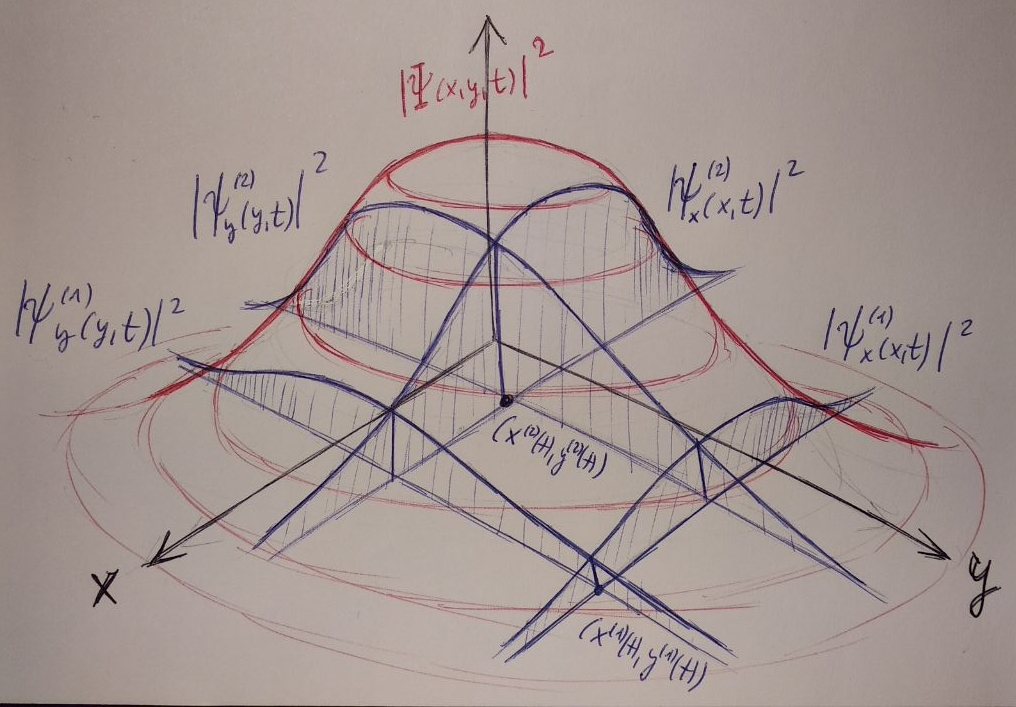
\includegraphics[width=0.65\linewidth]{slices.jpg}
  \caption{Depiction of the probability density of a 2D quantum system ($N=2$). In red the probability density of the full wave-function $\Psi(x,y,t)$ for a given time. In blue the pair of conditional wave-functions associated to two Bohmian trajectories $(x^{(1)}(t),y^{(1)}(t))$ and $(x^{(2)}(t),y^{(2)}(t))$ at a given time. Note that actually they coincide with other two trajectory's CWF-s at that time. }
  \label{fig:slices}
\end{figure}

\subsection*{(II.a.1) The Schrödinger Equation: Kinetic and Advective}
\addcontentsline{toc}{subsection}{(II.a.1) The Schrödinger Equation: Kinetic and Advective}
If we evaluate $\vec{y}(t,\vec{\xi})$ in the Schrödinger Equation, leaving $\vec{x}$ in the Eulerian frame:
\begin{equation}
i\hbar \pdv{}{t}\psi(\vec{x}, \vec{y}^\xi(t),t)=-\sum_{j=1}^m \frac{\hbar^2}{2m_j}\pdv[2]{}{x_j} \psi(\vec{x}, \vec{y}^\xi(t),t) + U(\vec{x}, \vec{y}^\xi(t),t)\psi(\vec{x}, \vec{y}^\xi(t),t) -\sum_{j=m+1}^N \frac{\hbar^2}{2m_j}\pdv[2]{}{x_j} \psi(\vec{x}, \vec{y},t)\Big\rvert_{\vec{y}^\xi(t)}
\end{equation}
Using that by the chain rule:
\begin{equation}
\dv{}{t}\psi(\vec{x}, \vec{y}^\xi(t),t)=\pdv{}{t}\psi(\vec{x}, \vec{y}^\xi(t),t)+\sum_{j=m+1}^N \pdv{}{x_j}\psi(\vec{x}, \vec{y},t)\Big\rvert_{\vec{y}^\xi(t)}\cdot \dv{}{t}x^\xi_j(t)
\end{equation}
We get:
\begin{equation}\label{KinAdvEL}
i\hbar \dv{}{t}\psi(\vec{x}, \vec{y}^\xi(t),t)=\qty[-\sum_{j=1}^m \frac{\hbar^2}{2m_j}\pdv[2]{}{x_j} + U(\vec{x}, \vec{y}^\xi(t),t)]\psi(\vec{x}, \vec{y}^\xi(t),t)+
\end{equation}
$$
+i\hbar\sum_{j=m+1}^N \pdv{}{x_j}\psi(\vec{x}, \vec{y},t)\Big\rvert_{\vec{y}^\xi(t)}\cdot \dv{}{t}x^\xi_j(t) -\sum_{j=m+1}^N \frac{\hbar^2}{2m_j}\pdv[2]{}{x_j} \psi(\vec{x}, \vec{y},t)\Big\rvert_{\vec{y}^\xi(t)}
$$
Where we define the so called Kinetic and Advective correlation potentials:
\begin{equation}\label{KinEL}
K(\vec{x}, \vec{y}^\xi(t),t)=-\sum_{j=m+1}^N \frac{\hbar^2}{2m_j}\pdv[2]{}{x_j} \psi(\vec{x}, \vec{y},t)\Big\rvert_{\vec{y}^\xi(t)}
\end{equation}
\begin{equation}\label{AdvEL}
A(\vec{x}, \vec{y}^\xi(t),t)=i\hbar\sum_{j=m+1}^N \pdv{}{x_j}\psi(\vec{x}, \vec{y},t)\Big\rvert_{\vec{y}^\xi(t)}\cdot \dv{}{t}x^\xi_j(t)
\end{equation}
We can see that equation \eqref{KinAdvEL} ruling the motion of the so called conditional wavefunctions $\psi(\vec{x}, \vec{y}^\xi(t),t)$ is almost a Schrödinger Equation for a system of $m$ dimensions (the Eulerian piece). The difference is that we now have two additional affine terms that actually depend on derivatives of the full wavefunction in the axes that we are considering in the Lagrangian frame. Clearly, if we want to compute these, we do not have enough with the conditonal wavefunction for a certain trajectory. 

The thing would be better if we also knew the value of the wavefunction at other points that are not the single $\vec{y}^\xi(t)$. Much in the same way that we did with the purely Lagrangian frame, for the piece considered with point-like trajectories, we will need to have several representatives to be able to approximate the derivatives in those directions.

Before further digging into the significance of this approach and how we could deal with this equation, let us review what we really mean by a conditional wavefunction.

\subsubsection*{What do we mean by a Conditional Wavefunction?}
\addcontentsline{toc}{subsubsection}{What do we mean by a Conditional Wavefunction?}
First of all, note that in the development of equation \eqref{KinAdvEL}, we considered no rule for the evolution of the trajectory $\vec{y}^\xi(t)$. In fact, we could impose the trajectories to be still (zero velocity field) or move them in custom paths (pre-defined velocity field). If we then evolve equation \eqref{KinAdvEL}, the values of the conditional wavefunction (CWF) $\psi(\vec{x}, \vec{y}^\xi(t),t)$ would reflect the value of the full WF over these custom trajectories for $y$. It is this freedom of choosing the motion of the Lagrangian elements $(\xi^x,\xi^y)$, that map the space for the degrees of freedom $\vec{y}$, that will allow us to build adaptive grids in a coming section.

Evolving trajectories with an arbitrary law of motion, even if would allow obtaining correct values for the wavefunction over the spots where they move, the trajectories themselves would not provide us much physical insight. We could nevertheless get more information about the dynamics if we made the velocity field depend on the wavefunction values at each point, on the properties of the dynamic fluid. We will see in the adaptive grid equations, that in fact we will be able to get information about a custom monitor function just from the movement of the trajectories. In particular, if we make the trajectories follow the flow lines of the fluid or Bohmian trajectories, we will get information of big interest. Why? Epistemologically, because these will be the trajectories that each particular experiment (each particular Universe) will take. Of course, experimental results will only reproduce stochastical results sampled from the density of the fluid, due to our lack of perfect knowledge of the position of all the particles in the Universe. However, this will allow us for instance to know about the past of a certain observation, about the dispersion or concentration of probability density etc. Bohmian trajectories accompanied by CWFs, or slices of the full WF could be useful to rebuild the full WF.

A very important point we should notice is that saying the Lagrangian part of the system $\vec{y}^\xi$ (the one that will be treated as an ensemble of particles) will follow probability density flow lines or Bohmian trajectories, is not that well defined, since we consider the rest of degrees of freedom in an Eulerian frame and their part of "trajectory" becomes undefined and asks for a further definition.



\subsubsection*{(a) If we only consider that there is trajectory in $\vec{y}$}

If we simply define the velocity field for $\vec{y}^\xi(t)=(x_{m+1}^\xi(t), ...,x_N^\xi(t))$ to be:
\begin{equation}
\dv{}{t}x_j^\xi(t)=\frac{1}{m_j}\pdv{S(\vec{x}, \vec{y})}{x_j}\Big\rvert_{\vec{y}^\xi(t)}=\frac{\hbar^2}{m_j}\Im\qty( \psi^{-1} \pdv{\psi}{x_j})\Big\rvert_{\vec{y}^\xi(t)} \quad j\in\{m+1,...,N\}
\end{equation}
We see that for each value of $\vec{x}=(x_1,...,x_m)$, the Eulerian degrees, we have a different velocity with which to move the trajectory in $\vec{y}$. In reality these velocities in $y$ for each $x$ are due to the fact that each $x$ can be seen as a fluid element if we make the degrees $x$ also Lagrangian. If this was so, each element of the CWF in $x$ should have its own trajectory in the $x$ axis, as we will see in (b). However, in this first view (a), we will assume there is only velocity field for the strictly Lagrangian coordinates. See Figure \ref{fig:only_y}.

If we took a CWF with an $m$ dimensional affine support, say with a certain initial $y^\xi(t_0)=:\xi_0^y$, we could parametrize it using a grid of elements $\xi^x_j$ to designate each point we consider in its discretization. We would find in the first time iteration of the CWF that each discrete element in $x$, each parametrized $\xi^x_j$, would be moved by a different velocity in $y$. Following these trajectories, what we would achieve as is shown in Figure \ref{fig:only_y}, is that each $x$ would always maintain a single value of the wavefunction, because the $x$ points are fixed, meaning each elemnt identified by $\xi^x_j$ will continue having $x=\xi^x_j$ at all times. However, the "slice" would see its affineness destroyed. The evolution of the CWF would describe the evolution of a function graph in $x$, in the sense that each $x$ would still have a single complex wavefunction value (even if it would loose the affine structure).

\begin{figure}[h!]
  \centering
    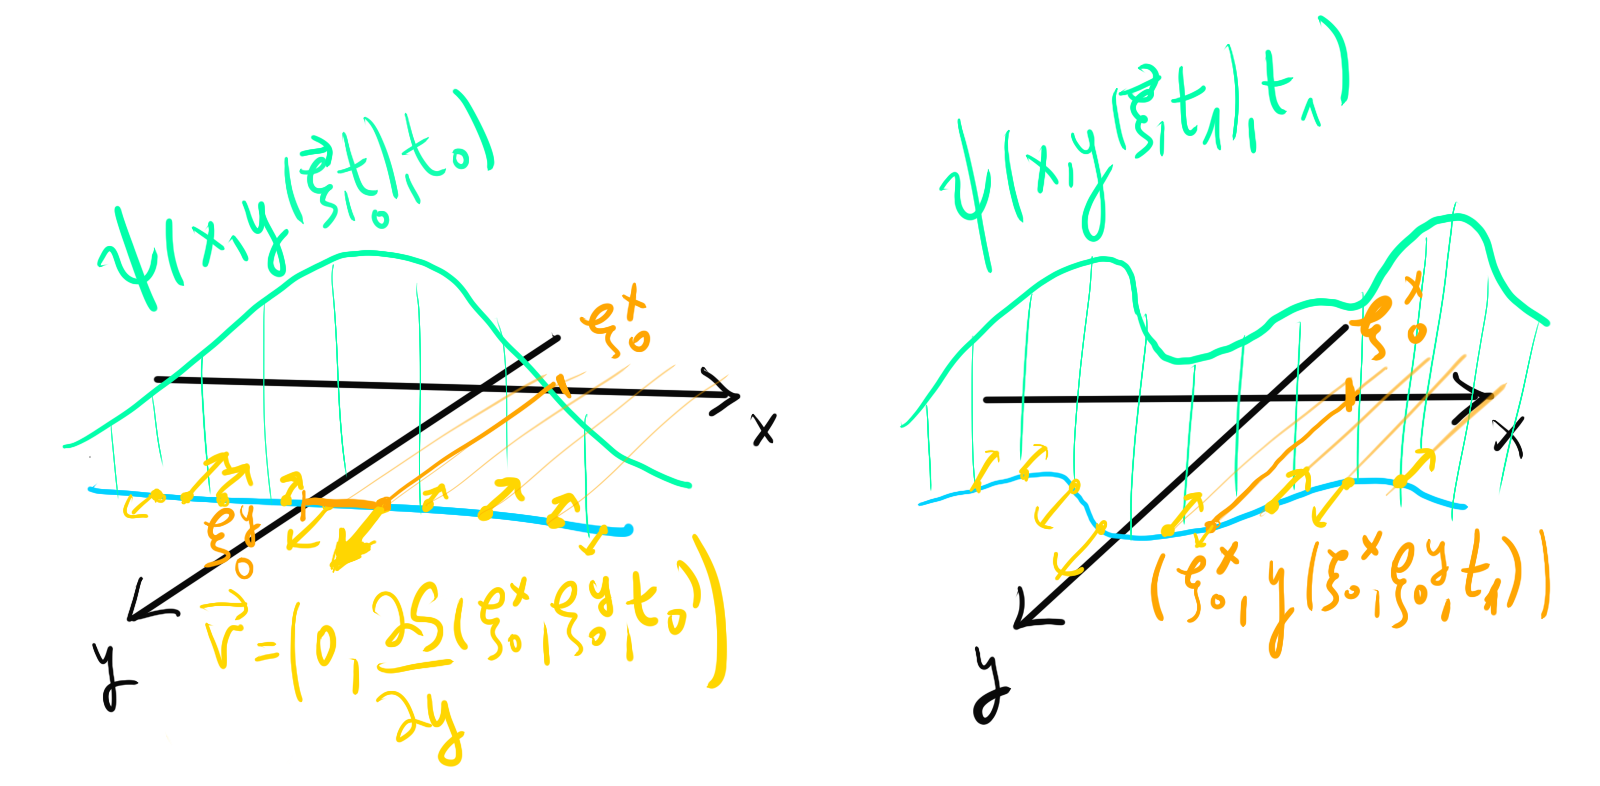
\includegraphics[width=0.65\linewidth]{unstructure_aligned.png}
  \caption{The blue line represents the $m$ dimensional support of the CWF that is conditioned to have $y=\xi^y_0$ at $t=t_0$ (in the left). In green we see the magnitude of the complex CWF plotted over the support of the CWF (the slice of the full WF). In yellow we see the velocity vectors that will move each element of the CWF, each parametrized $\xi^x_j$. We see in the right the time $t_1>t_0$. Note haow the elements $\xi^x_j$ always preserve their $x=\xi^x_j$ value, that is, they strictly move in $y$. }
  \label{fig:only_y}
\end{figure}

If we tried to understand what really is happening from a fully Bohmian trajectory perspective, it is certain that we are not evolving Bohmian trajectories of the full system, since we are restricting the movement of the fluid elements in $y$. It is as if trajectories were impeded to be moved in $x$. This means that the trajectories obtained in the Lagrangian axes would not be Bohmian trajectories. However, if we are really to treat the Eulerian degrees $x$ as not part of a fluid, this would be the way to go.

A good thing about this would be that if we evolved several CWF-s for different initial positions in $y^\xi(t_0)=\xi^y_k$, the discretized $x$ points would always be aligned between the CWF-s, with the advantage that computing derivatives $\pdv{}{y}$ or interpolating in $y$ would be simplified, even if the $y$ grid for each $x$ would get unstructured with time. See Figure \ref{fig:only_y_grid}

\begin{figure}[h!]
  \centering
    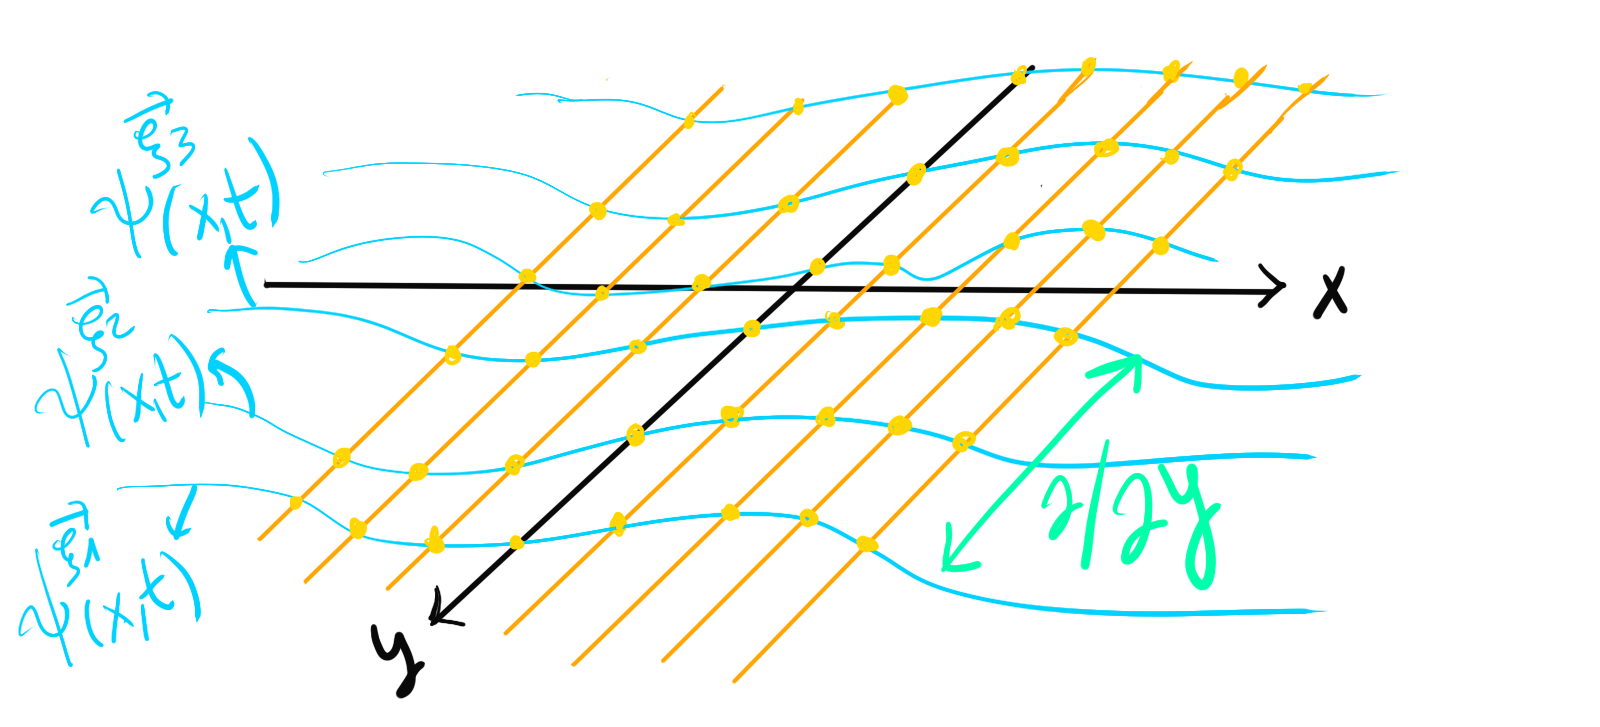
\includegraphics[width=0.65\linewidth]{aligned.png}
  \caption{Blue lines represent the suppoort of CWF-s with different initial time $\xi^y_j$ after they evolve in time following  \eqref{a}. Note how the discretized points of all the CWF-s, the yellow dots, are aligned even at $t>t_0$, meaning operations like $\pdv{}{y}$ on each yellow element can be trivially done numerically. }
  \label{fig:only_y_grid}
\end{figure}

Thus the trajectories we obtain for $y^\xi$ are certainly not Bohmian trajectories, since we are forcing $x$ positions to be still. Mathematically what we are doing is:
\begin{equation}\label{a}
\begin{cases}
\vec{x}^\xi(t)=\vec{\xi}_x \quad \forall t\geq t_0\\
\vec{y}^\xi(t)=\vec{\xi}_y+\int_{t_0}^t \vec{v}_y(\vec{x}, \vec{y}(t),t)dt\\ \\
v_j(\vec{x}, \vec{y},t)=\frac{1}{m_j}\pdv{S(\vec{x}, \vec{y},t)}{x_j}\quad j\in\{m+1,...,N \}
\end{cases}
\end{equation}

\subsubsection*{(b) If we consider that there is trajectory in $\vec{\x}$}
What if we allowed the elements of the CWF-s to move in $x$ as well? (following Bohmian velocity fields). We would have that:
\begin{equation}
\begin{cases}\label{b}
\vec{x}^\xi(t)=\vec{\xi}_x +\int_{t_0}^t \vec{v}_x(\vec{x}(t), \vec{y}(t),t)dt\quad \forall t\geq t_0\\
\vec{y}^\xi(t)=\vec{\xi}_y+\int_{t_0}^t \vec{v}_y(\vec{x}(t), \vec{y}(t),t)dt\\ \\
v_j(\vec{x}, \vec{y},t)=\frac{1}{m_j}\pdv{S(\vec{x}, \vec{y},t)}{x_j}\quad j\in\{1,...,N \}
\end{cases}
\end{equation}

As it can be seen in Figure \ref{fig:fallback}, each element of the initially affine support manifold for the CWF (blue in the Figures), would move in different directions in configuration-space. The CWF would evolve at each point following the fluid flow and the data would turn into an unstructured grid in all axes, even in the Eulerian $x$. We would now have a varying number of values of wavefunction per $x$ as a function of time (several yellow dots per $x$). It would still be an $m$ dimensional manifold, meaning the parametrization given by $\vec{\xi}^x_j$ would still be valid, and we would still have one point in the wavefunction per each  $\vec{\xi}_x$ in the initial manifold. However, as said, a certain $x$ would now be possible to have multiple wavefunction evaluations. For all practical means we would have falled back to the fully Lagrangian frame, where we had independent fluid elements moving in configuration-space! Performing derivatives in $y$ in order to evolve the CWF with \eqref{KinAdvEL} would now be a very difficult task even using many different CWF-s, as the WF values per $x$ would no longer need to be aligned.

\begin{figure}[h!]
  \centering
    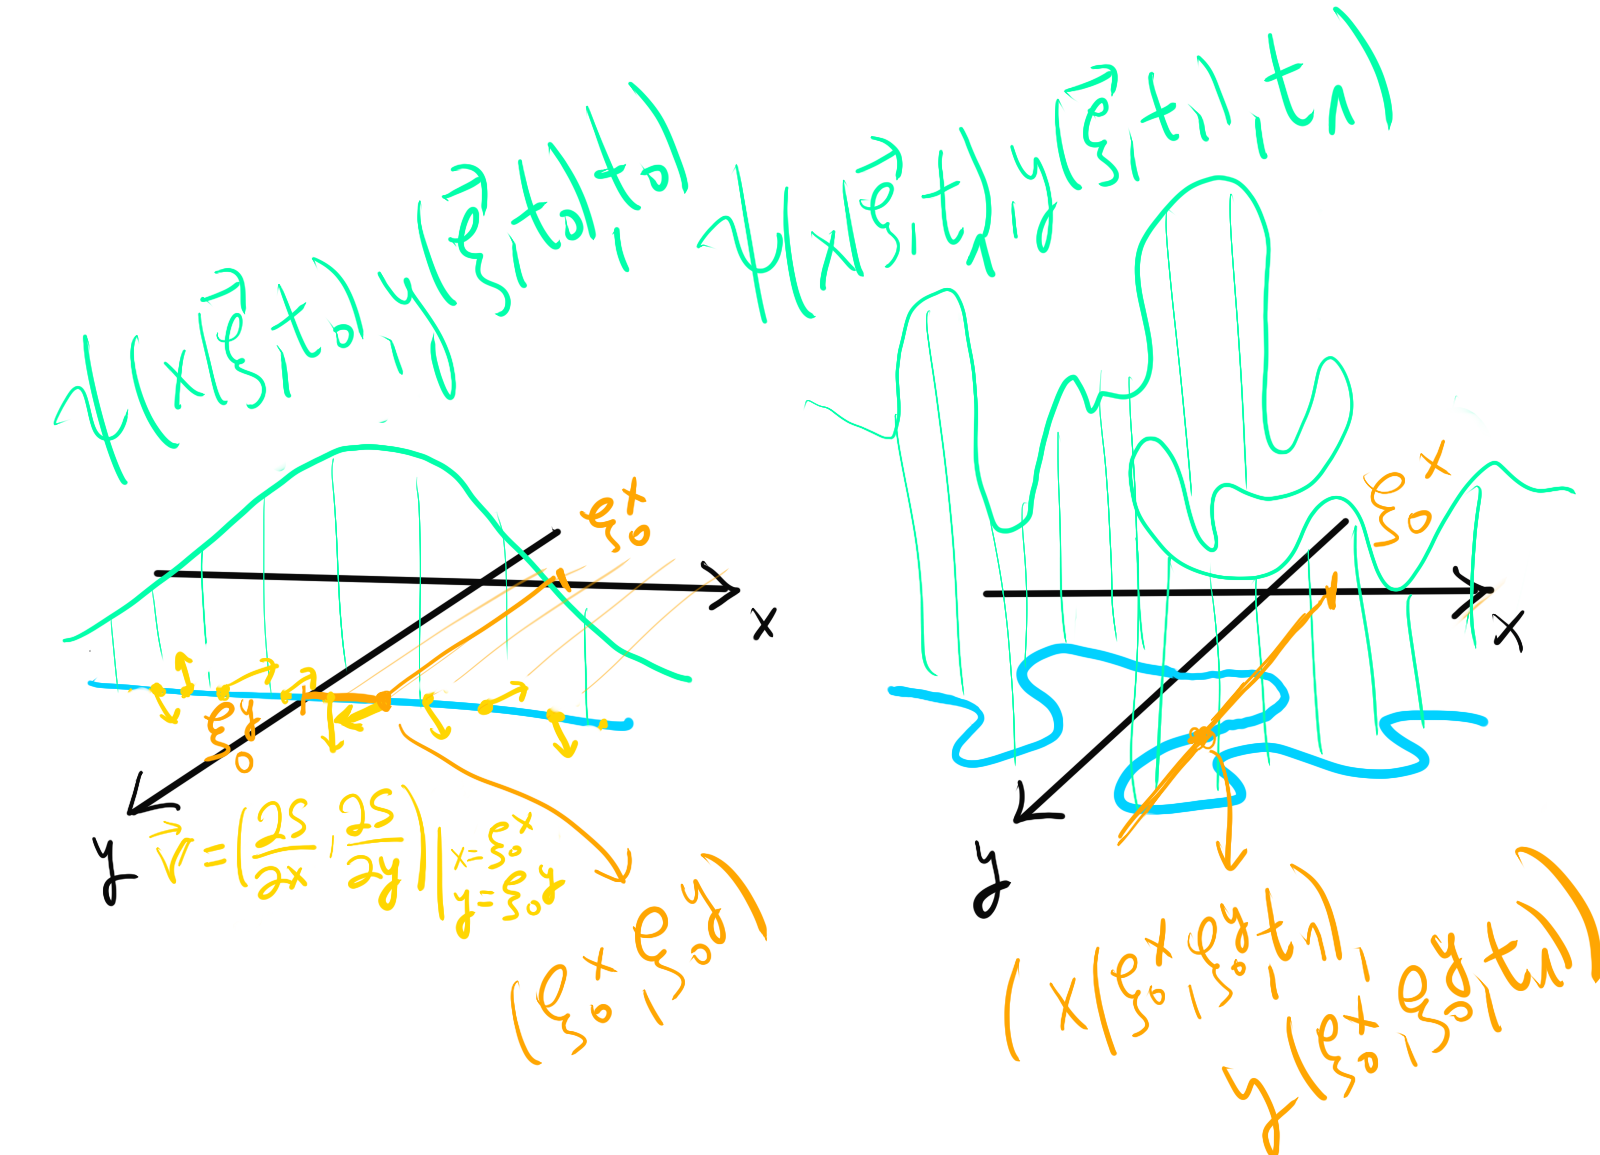
\includegraphics[width=0.65\linewidth]{unstructuring.png}
  \caption{Left $t=t_0$, right $t=t_1$. In blue, the $m$ dimensional support of the CWF. In green the field value at each point (say the phase or magnitude of the WF). In yellow the elements of the CWF we consider, together with the velocity vectors we will use to move them according to \eqref{b}. Note how each fluid element moves independently, unstructuring the grid they compose not only in $y$ as happened in (a), but also in $x$, just like with the fully Lagrangian study-case. }
  \label{fig:fallback}
\end{figure}

\subsubsection*{(c) If we consider that each CWF moves along a single trajectory}
In (a) we found that part of the system was really in the Eulerian frame and part was really in the Lagrangian one. However, the trajectories we evolved were not useful. In (b) we found that having really Bohmian trajectories move each point of the CWF resulted in the fully Lagrangian frame. However, notice that this was only because we allowed each point of the CWF to move along the flow lines. What if we forced all the points of the CWF to move together along a single Bohmian trajectory, a single flow line?

Notice one of the most interesting properties of the CWF-s: a single slice, a single CWF is enough to define the velocity field in $x$. The (Bohmian) velocity field is due to a derivative in the $x$ axis, $\pdv{S(x,y^\xi(t),t)}{x}$, and we are treating this axis in the Eulerian frame (thus we know its values along all $x$ for this $y^\xi(t)$). So in principle, knowing an affine CWF slice lets us know the $x$ velocity field for any $x$ on the slice!  But again, if we simply define the velocity field in $x$ for each and every $x$ and move them accordingly we will loose the regular grid. What we can do is the following: define just one trajectory in $x$ for the CWF. That is, choose one $\xi_x$ at random appart from the $\xi^y_0$ we already chose and use the CWF to propagate $\vec{x}^\xi(t)$ in time. Then we know a single point $x$ where we are interested to know the velocity field in $y$ for the initial $\xi^y_0$, we no longer need to attribute each point in the CWF a different velocity. This way, at all times we will only have a single trajectory to track, and in fact it will be a Bohmian trajectory by definition. That is, the CWF will move in space preserving its affine shape and it will not get branched in several $y$ trajectories. See Figure \ref{fig:singleTraj}.

\begin{figure}[h!]
  \centering
    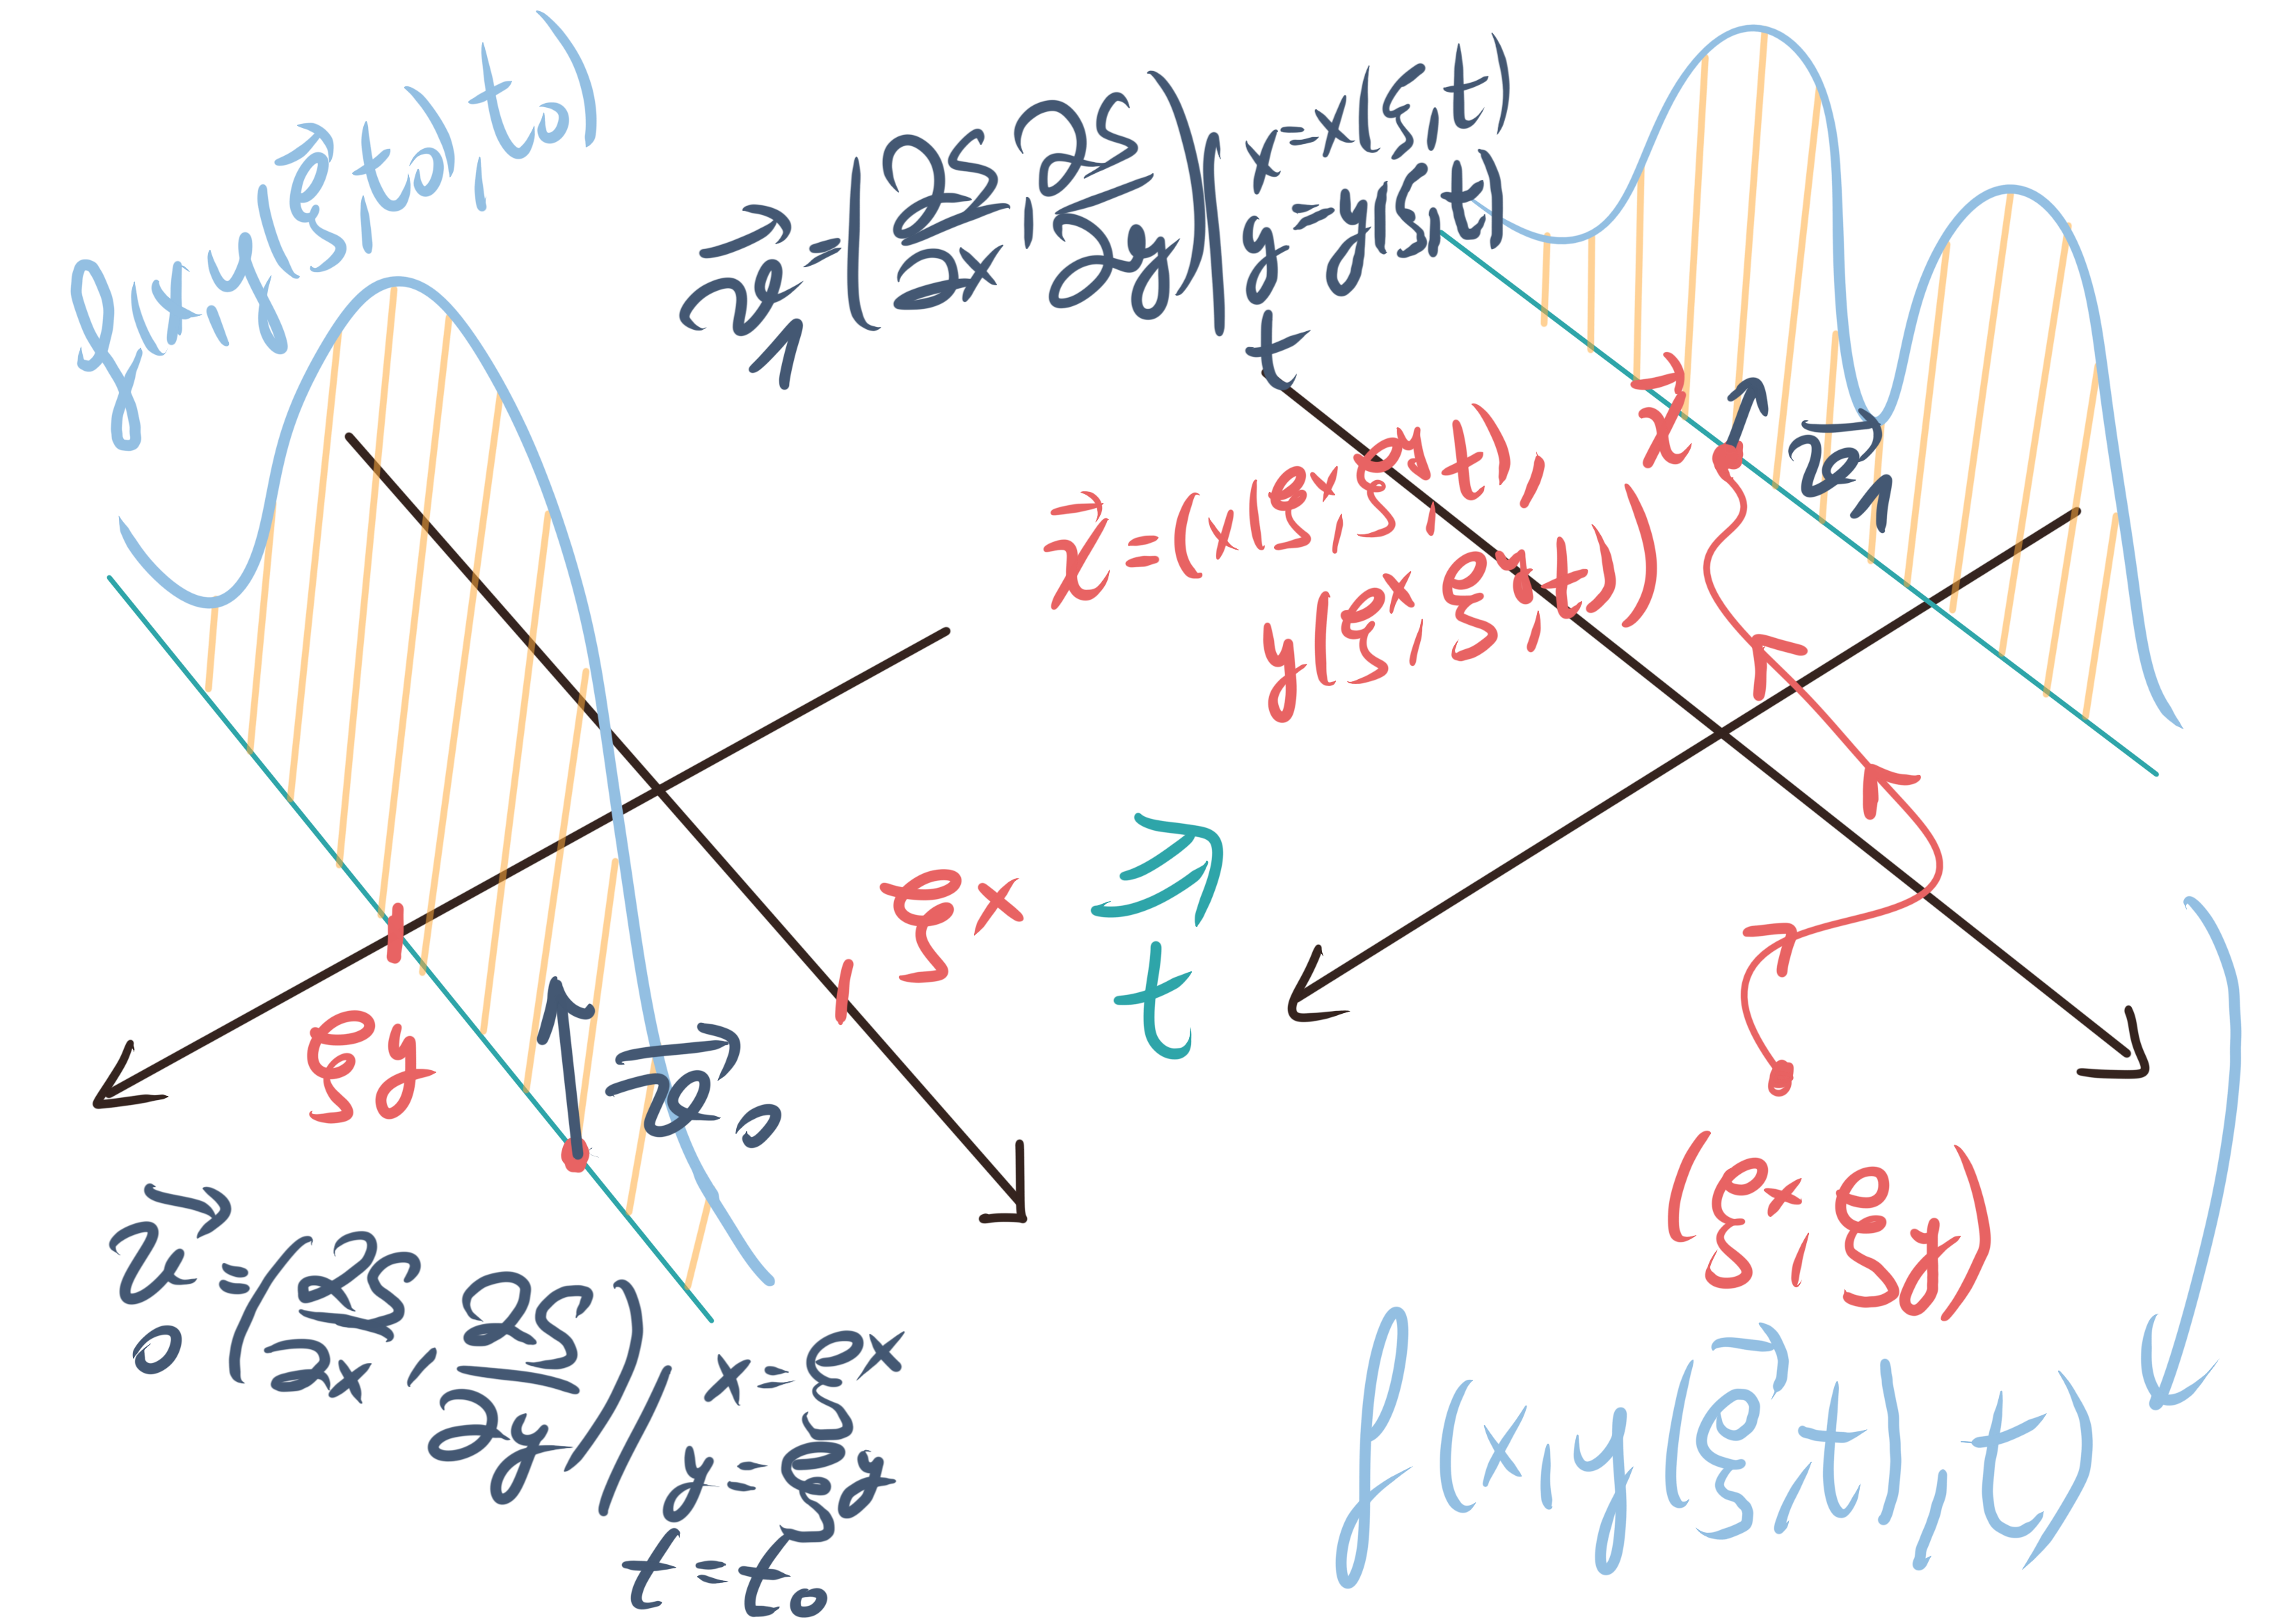
\includegraphics[width=0.65\linewidth]{moving_bohmian.png}
  \caption{Right $t=t_0$, left $t=t_1$. In blue, the support of the CWF, which can be seen to have its affinity preserved at all times. This is because the whole CWF is displaced following the same Bohmian trajectory as explained in (c): the one for $(\xi^x_0, \xi^y_0)$. In green the value of a property of the WF over the support of the CWF. We see that the $x$ velocity of the trajectory is fully given by the variation of the CWF. For the velocity in $y$ however, we still have the problem that we are only dealing with a single slice and thus cannot have local information of first or higher order. }
  \label{fig:singleTraj}
\end{figure}

\subsubsection*{(d) Two Coupled Conditional Wavefunctions?}

We now accept that in order to preserve a half Eulerian half Lagrangian frame feasible and still obtain Bohmian trajectories, we need to evolve only one Bohmian trajectory per CWF, move the whole CWF along a single trajectory. We also know that the CWF is enough to get the velocity field in its Eulerian degrees of freedom, {\bf but not} for the Lagrangian degrees of freedom, since we only posses information of "zeroth order", a single slice in the Lagrangian axis. For those degrees of freedom we have the same problem that we had in the fully Lagrangian: we will need several trajectories, several CWF-s to approximate the derivatives. Now, if we will only evolve a single trajectory per CWF: couldn't we evolve a coupled CWF with the Eulerian degrees being the Lagrangian of the first and vice versa? See Figure \ref{fig:pair_bohm}. This way, we could get the velocity field that guides the joint trajectory, just knowing this pair of CWF-s! We would not need any further interpolation or more CWF-s to evolve the trajectory (to know the velocity field)!

\begin{figure}[h!]
  \centering
    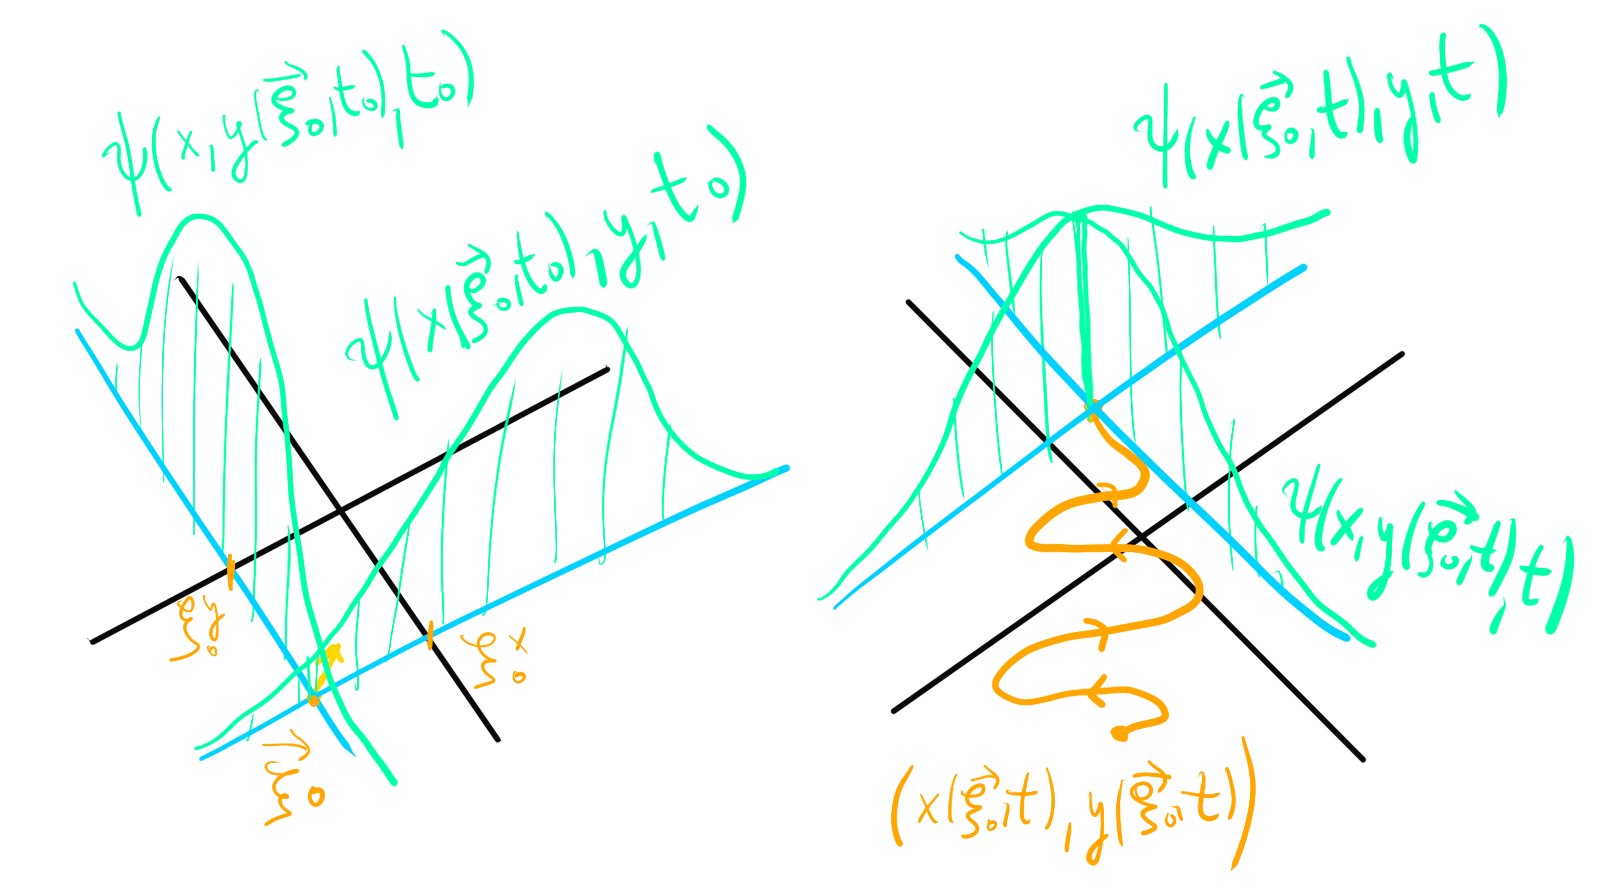
\includegraphics[width=0.65\linewidth]{bohmian_pair.png}
  \caption{Following the same caption of Figure \ref{fig:singleTraj}, we see that having a complementary CWF that has as Lagrangian degrees of freedom the Eulerian ones of the first, allows the evolution of the common trajectory with no further requirements. Note how the WF value at the trajectory position for both CWF-s should coincide. The difference of these could be a metric to be used in numerical simulations.  }
  \label{fig:pair_bohm}
\end{figure}

Well, it is true that we need no more information to get the velocity fields, than these two CWF-s, however, in order to evolve the CWF-s themselves \eqref{KinAdvEL}, we need to know the derivatives of the WF in the Lagrangian directions $y$, not only for the point $x$ of the trajectory, but for all $x$ points in the CWF! But it is a good point to start with.

Mathematically, if we choose a certain initial point for the trajectory moving a pair of CWF-s: $\vec{\xi}=(\vec{\xi}_x, \vec{\xi}_y)$ we can define the CWF-s as:
\begin{equation}
\psi_x^\xi(\vec{x},t):=\psi(\vec{x}, \vec{y}^\xi(t),t) \text{  and  } \psi_y^\xi(\vec{y},t):=\psi(\vec{y}, \vec{x}^\xi(t),t)
\end{equation}
Then the trajectory $(\vec{x}^\xi(t), \vec{y}^\xi(t))$ will be entirely determined by the CWF pair following:
\begin{equation}
\begin{cases}\label{d}
\vec{x}^\xi(t)=\vec{\xi}_x +\int_{t_0}^t \vec{v}^x(\vec{x}^\xi(t), \vec{y} ^\xi(t),t)dt\quad \forall \\
\vec{y}^\xi(t)=\vec{\xi}_y+\int_{t_0}^t \vec{v}^y(\vec{x}^\xi(t), \vec{y}^\xi(t),t)dt\\ \\
v_j^k(\vec{x}, \vec{y},t)=\frac{1}{m_j}\pdv{S^x(\vec{x}, \vec{y},t)}{x_j}= \frac{\hbar^2}{m_j}\Im\qty( \psi_k^{-1} \pdv{\psi_k}{x_j})\Big\rvert_{\vec{y}^\xi(t)} \quad k\in\{ x,y\}\ \ j\in\{ 1,..,N\}
\end{cases}
\end{equation}

Looking back at equation \eqref{AdvEL}, guiding the time evolution of the CWF-s, we notice that we will still lack the knowledge of the derivatives in $y$ for all $x$ except for the one where the trajectory currently is. Then once again, the solution will be to evolve several trajectories using their coupled CWF-s in paralell for each time iteration and use all of them to approximate the derivatives in their Lagrangian axes, just like we did in the previous Section. This is depicted in Figure \ref{fig:manyBohmian}.

\begin{figure}[h!]
  \centering
    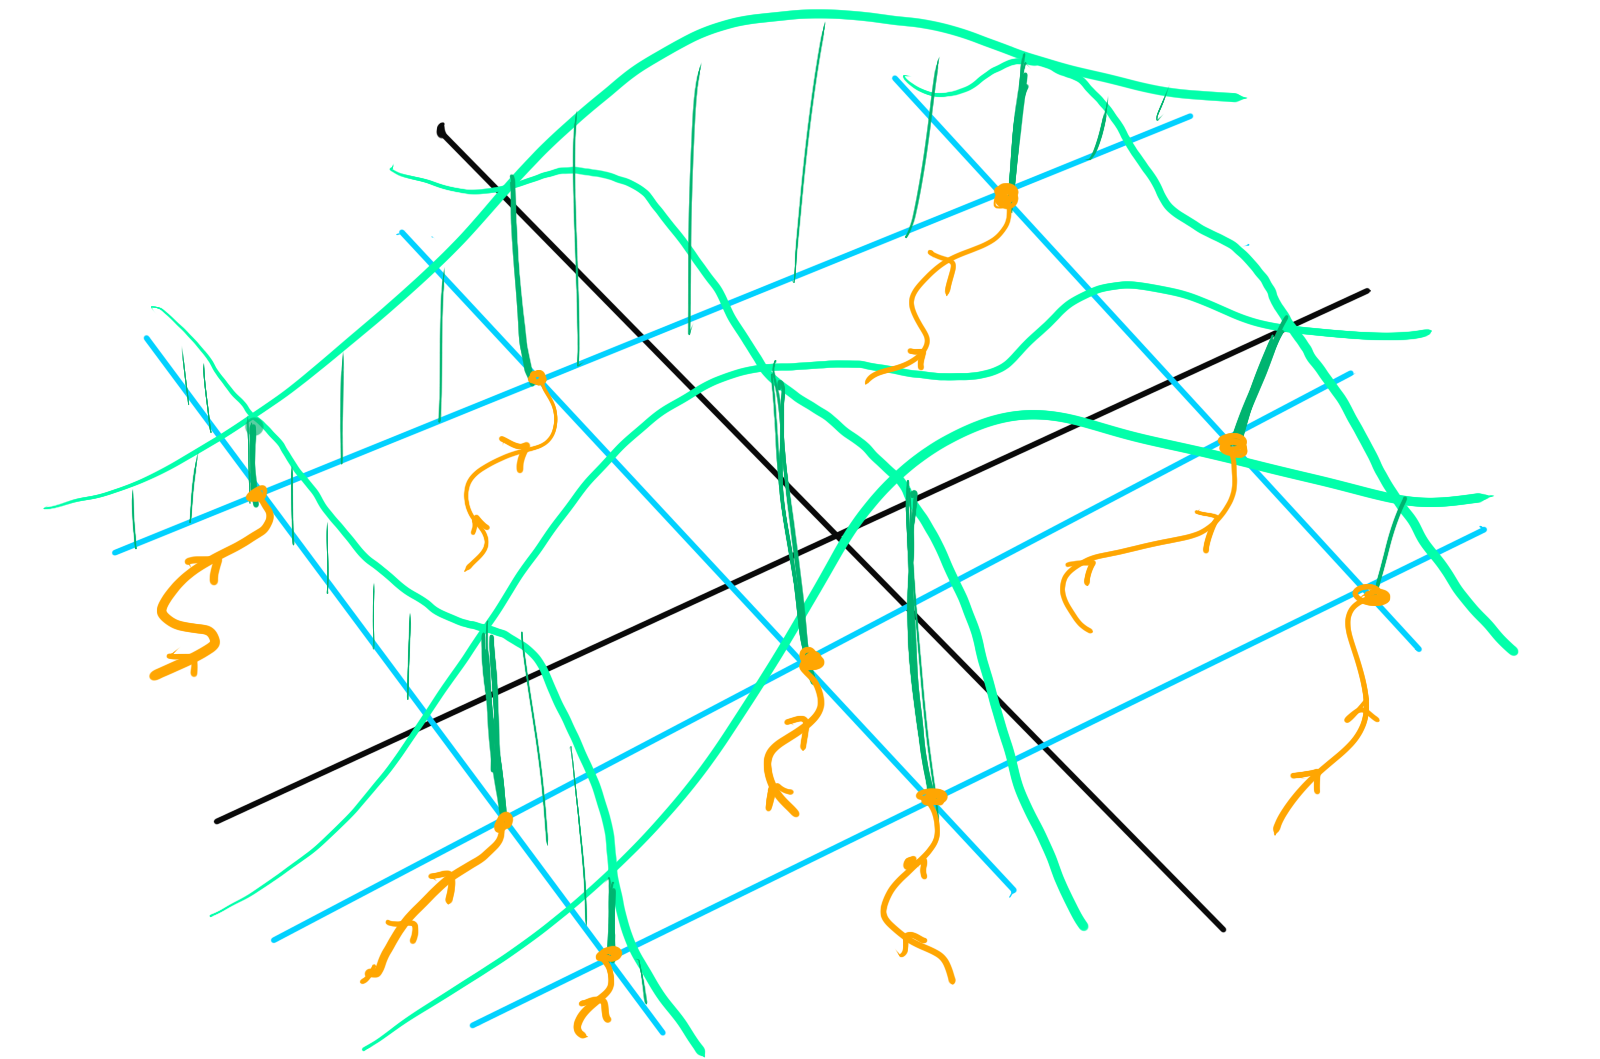
\includegraphics[width=0.65\linewidth]{many_bohmian.png}
  \caption{In blue we can see the affine supports of several pairs of CWF-s (slices of the WF) built by following \eqref{d}. In each intersection we have enough information as for evolving a Bohmian trajectory. }
  \label{fig:manyBohmain}
\end{figure}

In Figure \ref{fig:aligned}, we can see how several CWF-s could be used in order to have information to compute derivatives in all the directions. However, it is clear that in some particular points, we will have a bigger density of aligned points. This could be aliviated by using an approach we will explain in the next gray-box, consisting on leaving the trajectories still.


\begin{figure}[h!]
  \centering
    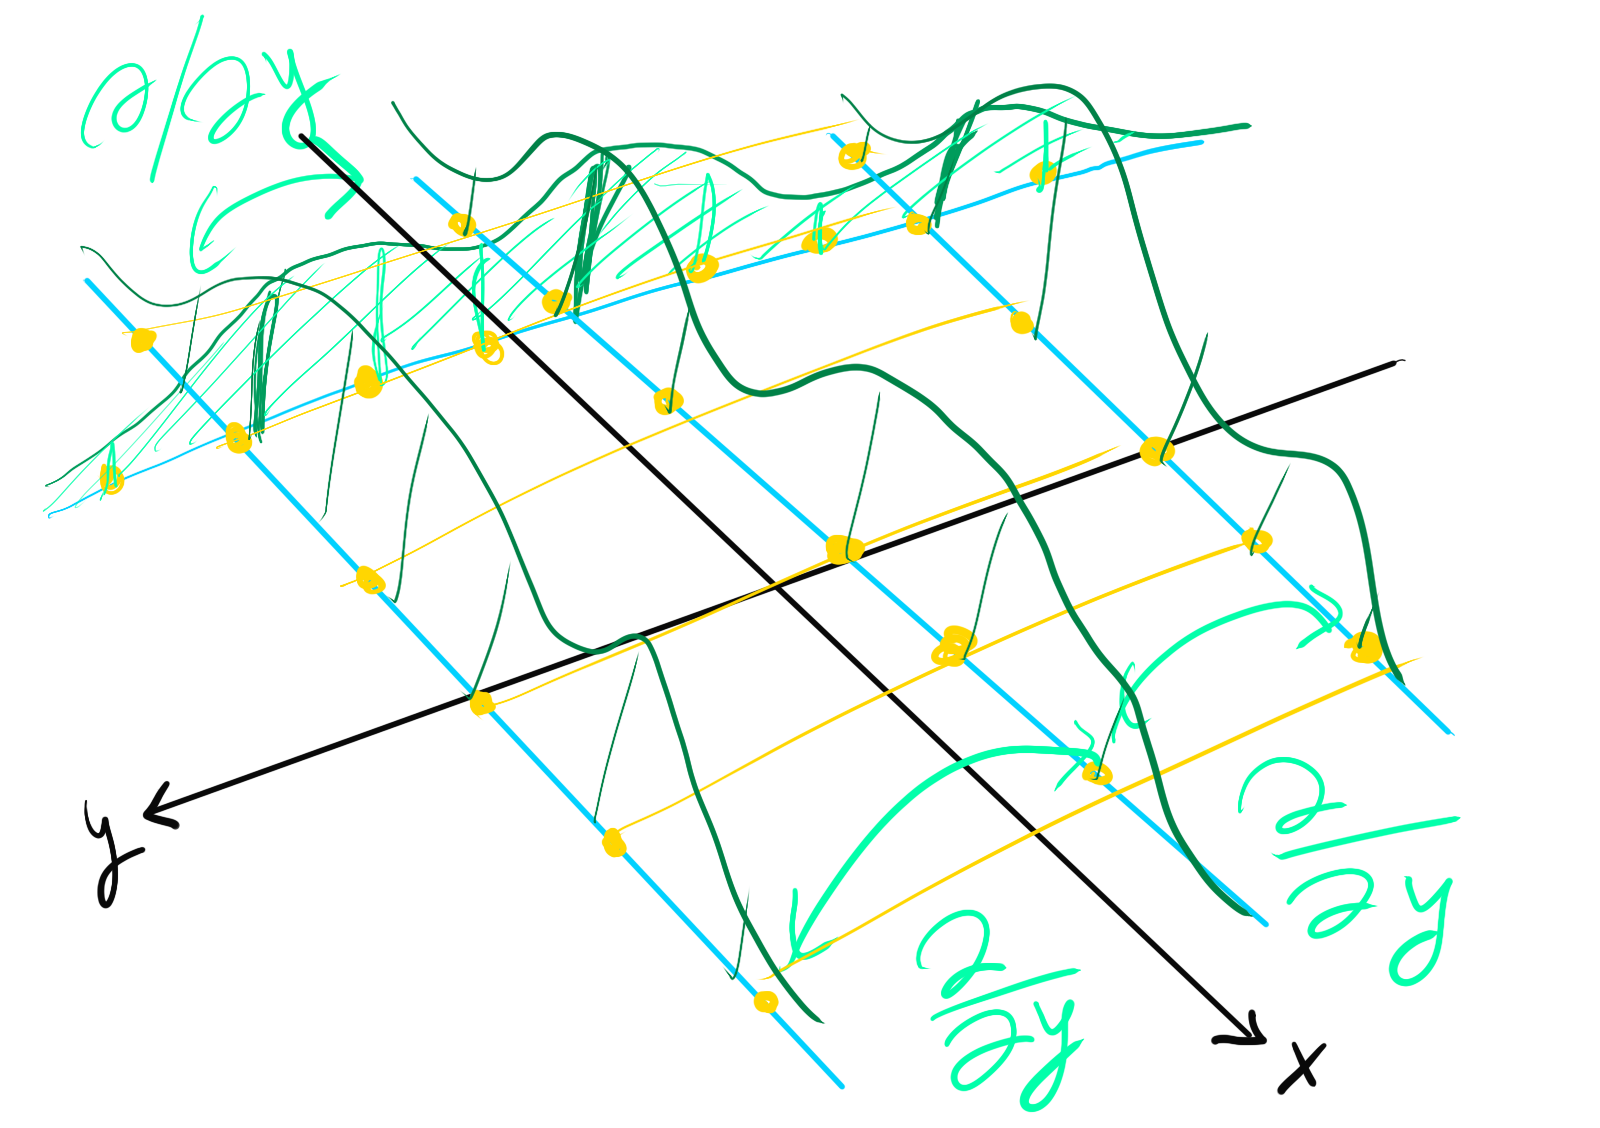
\includegraphics[width=0.65\linewidth]{aligned_original.png}
  \caption{In blue we can see several CWF-s (their supports). Yellow dots show the discrete elements of the CWF-s we will consider. This image shows two things: 1. parallel CWF-s (CWF-s with the same Lagrangian degrees but different initial positions) can be used to approximate derivatives in the Lagrangian directions $\pdv{}{y}$. 2. Crossed CWF-s with complementary Lagrangian degrees can be used also to approximate derivatives in the Lagrangian directions with a higher degree of precision than using parallel CWF-s.  }
  \label{fig:aligned2}
\end{figure}

\subsubsection*{(e) n Conditional Wavefunctions Coupled by a Single Bohmian Trajectory}
In fact, we could do the previous trick by evolving not two, but $n$, up to $N$ coupled different CWF-s with a single Bohmian trajectory, where each CWF could have different Eulerian dimensionalities. For example, we could evolve $N$ CWF-s, where each has a different single Eulerian dimension (a 1D CWF): each of them would give us the information in its Eulerian axis to evolve the common Bohmian trajectory.

Then if we chose $n=N$ we would have a 1D Eulerian CWF per axis. {\bf If we chose $n=N/3$ we could have one 3D Eulerian CWF per 3D physical space particle}, all of them coupled by a single global Bohmian trajectory. This in particular could be an interesting one following the ideas in Ref. \cite{physicalOriols}. We could have even stranger combinations like the one shown in Figure \ref{fig:strangeSlicing}. All of them would allow the proper time evolution of a single Bohmian trajectory.
\begin{figure}[h!]
  \centering
%    \includegraphics[width=0.65\linewidth]{strangeSlicing.png}
  \caption{K }
  \label{fig:strangeSlicing}
\end{figure}

% Faltan, figura pa slices, pa strange slicing y añadirles los yellow dots en la del descalabro.


\subsubsection*{What is the advantage of the Half Lagrangian-Half Eulerian approach?}
The advantage is that we might be able to get the best of both worlds: the Eulerian and the Lagrangian.

\begin{itemize}
\item The more dimensional the CWF's Eulerian degrees are, the smaller the space for sampling the trajectories of the Lagrangian part will be. This means that the less CWF-s will be required to reproduce the full wavefunction or to achieve a certain precision in the derivatives in Lagrangian directions. However, the more computationally complex will be the CWF-s to evolve, so the problem gets more complex to be parallelized. In the limit, of $m=N$ we would recover the linear Schrödinger equation in the Eulerian frame, which scales exponentially in time with dimensions.

\item The less dimensional the CWF's Eulerian degrees, the more trajectories we will need to reconstruct the full wavefunction and to get the derivatives in the Lagrangian directions, in fact, presumably exponentially more. However, the CWF-s will be simpler to evolve and as the trajectories can (and must) be computed coupled but in parallel, the more of exponential complexity we will transfer to parallel threads. In the limit of $m=0$, we recover the fully Lagrangian frame, where we achieve the apparently highest parallelizability of the Quantum many body problem.

\item Unlike the fully Lagrangian frame, in this case, each Bohmian trajectory is accompanied by lots of wavefunction points (not just one) and therefore, interpolating the full wavefunction is way simpler, by for instance a nearest neighbour approach. Each CWF is a full $mD$ affine hyperplane of values for the wavefunction.

\item The grid is preserved in a structured manner at all times for the Eulerian degrees, while it gets unstructured for the Lagrangian axes. However, if coupled CWF-s are present, there are parts of the Lagrangian axes for one CWF that are Eulerian for the other, so there is always track of the wavefunction in all the extent of the simulation domain. The intersting thing is that the points in x of different trajectory CWF-s are always aligned, so the numerical derivatives in y or interpolations are ways impler than in a fully unstructured grid.

\item {\bf Fast and Slow Degrees of Freedom}: CWF-s provide a natural way to treat the slow degrees of freedom separated form the fast ones, like an atom nuclei from the orbiting electrons. It is common in molecular dynamics algorithm to consider classical trajectories for parts of the quantum system and quantum wavefunctions for other parts. We will see how we could do this using CWF-s in the Bohmian Newton's Equation.
\end{itemize}

% FALTAN COMENTS EN SE QTM Y AKI DE LA COMPLEJIDAD Y PARALELIZABILIDAD. Y LA TRANSFERENCIA ENTRE INTEGRAL EIGENSTATE COMPUTATION Y ESTO Y LO OTRO KIZAS ESO LO PODRIA HACER AL FINAL MEJOR SUPONGO.



\subsection*{(II.a.2) The Schrödinger Equation: G and J Correlations}
\addcontentsline{toc}{subsection}{(II.a.2) The Schrödinger Equation: G and J Correlations}
In this section we will describe the Lagrangian degrees of freedom using the density and action, while the Eulerian part will be described by a wavefunction. 

Following the development in Chp.1 V 6 of \cite{JordiXO}: We can try to find a Schrödinger like equation for the CWF-s employing the following "trick". An arbitrary non-zero single valued complex function $f(x, t):\R^m \rightarrow \C$ can be imposed to be the solution of an mD Schrödinger equation:\vspace{-0.3cm}
$$
i \hbar \pdv{f(x,t)}{t} = -\sum_{k=1}^m\frac{\hbar^2}{2 m_k}\pdv[2]{f(x,t)}{x_k} + W(x,t) f(x,t)
$$
if the potential term $W(x, t)$ is defined as:\vspace{-0.3cm}
$$
W(x, t) := \qty(i \hbar \pdv{f(x,t)}{t} +\sum_{k=1}^m\frac{\hbar^2}{2 m_k}\pdv[2]{f(x,t)}{x_k} ) \frac{1}{f(x,t)}\vspace{-0.3cm}
$$
The proof is immediate. An observation that we must note is that for an arbitrary $f(x,t)$, the potential $W(x,t)$ can be complex. This is not the case in the usual Schrödinger Equation.

If we now take the CWF where we had $m$ Eulerian degrees of freedom $x$ and $N-m$ Lagrangian degrees of freedom $y$ and write it in polar form: $\psi(x, y^\xi(t),t)=:\psi^\xi (x,t)=\p^\xi(x,t) e^{i\z^\xi(x,t) / \hbar}$, we can introduce it in this general complex potential $W^\xi(x,t)$:
$$
W^\xi(x, t) = \qty(i \hbar \pdv{\psi^\xi (x,t)}{t} +\sum_{k=1}^m\frac{\hbar^2}{2 m_k}\pdv[2]{\psi^\xi (x,t)}{x_k} ) \frac{1}{\psi^\xi (x,t)} = \qty(i \hbar \pdv{\qty(\p^\xi e^{i\z^\xi/\hbar})}{t} +\sum_{k=1}^m\frac{\hbar^2}{2 m_k}\pdv[2]{\qty(\p^\xi e^{i\z^\xi/\hbar})}{x_k} ) \frac{1}{\p^\xi e^{i\z^\xi/\hbar}}
$$
using the Leibniz derivation rule several times and an inverse chain rule, rearranging we arrive at:
$$
W^\xi(x, t)=-\sum_{k=1}^m\frac{1}{2m_k} \qty( \qty(\pdv{\z^\xi}{x_k})^2 -\frac{\hbar^2}{\p^\xi}\pdv[2]{\p^\xi}{x_k})\ -\pdv{\z^\xi}{t}+ \ i \ \frac{\hbar}{\p^{\xi\ 2}} \qty(\pdv{\p^{\xi\ 2}}{t}+\sum_{k=1}^m\pdv{}{x_k}\qty(\frac{\p^{\xi\ 2}}{m_k}\pdv{\z^\xi}{x_k}))
$$
%Separating the real and imaginary parts:
%$$
%\begin{cases}
%\mathbb{R}e\{W(x,t)\}=-\pdv{\z^\xi(x,t)}{t}-\frac{1}{2m_a} \qty( \qty(\pdv{\z^\xi(x,t)}{x_a})^2 -\frac{\hbar^2}{\p^\xi(x,t)}\pdv[2]{\p^\xi(x,t)}{x_a})\vspace{-0.3cm} \\ \\
%\mathbb{I}m\{W(x_a, t)\} = \frac{\hbar}{\p^\xi(x,t)^2} \qty(\pdv{\p_a^2}{t}+\pdv{}{x_a}\qty(\frac{\p_a^2}{m_a}\pdv{\z_a}{x_a}))\vspace{-0.1cm}
%\end{cases}
%$$
%Where we can recognize the \ref{QHJE} for a single particle in 1D. As such, the real part of W is simply the scalar real potential, then the Hamiltonian, followed by the kinetic energy and the quantum potential of a 1D particle.
%Which is clearly a modified particle conservation equation \ref{CE}. Note how if  $Im\{W(x_a, t)\} =0$ then we get the common continuity equation, which would mean that probability is conserved, and the solution $\Phi(x,t)$ would preserve its norm at all times (the conditional $r_a^2$ would integrate a same norm at all times in its spatial dimension $x_a$). Nonetheless, if $Im\{W(x_a, t)\} \neq 0$, then particles/probability are NOT conserved, and their source or sink will be quantified by $\frac{2 \_a^2}{\hbar} Im\{W(x_a, t)\}$. Therefore, the norm of $\psi^\xi (x,t)$ will not need to be preserved in the time evolution. \vspace{-0.3cm}\\

If $W^\xi$ has that shape, $\psi^\xi (x,t)$ will be the solution of the differential equation:\vspace{-0.2cm}
$$
i \hbar \pdv{\psi^\xi (x,t)}{t} = -\sum_{k=1}^m \frac{\hbar^2}{2 m_k}\pdv[2]{\psi^\xi (x,t)}{x_k} + W^\xi(x,t) \psi^\xi (x,t)\vspace{-0.2cm}
$$
which if $\mathbb{I}m\{W^\xi\} =0$ would look like an actual mD Schrödinger Equation. However, $W^k$ depends on parts of the CWF itself, so the differential equation is  {\bf non-linear} even in that case.

We can further develop the expression of $W^\xi$ using the conditional definition of $\psi^\xi$. Note that $\psi^\xi ( x, t) := \Psi(x, y^\xi(t),t)$ means that $\z^\xi(x,t)=S(x, y^\xi(t),t)$ and $\p^\xi (x,t)=R(x, y^\xi(t),t)$, where we have that the full wavefunction in polar form is $\Psi(x,y,t)=R(x,y,t)e^{iS(x,y,t)/\hbar}$. Carefully evaluating them in $W^\xi$ and applying the chain rule, the real part of $W^\xi(x,t):=\W(x,y^\xi(t),t)$ yields:
$$
\R e\{W(x,t)\}=\R e\{\W(x, y^\xi(t),t)\}=\vspace{-0.12cm}
$$
$$
\sum_{a=1}^m \Big\{-\frac{1}{2m_a} \qty(\pdv{S(x, y^\xi(t),t)}{x_a})^2 +\frac{\hbar^2}{2m_aR(x,y^\xi(t),t)}\pdv[2]{R(x, y^\xi(t),t)}{x_a}\Big\}-\dv{S(x,y^\xi(t),t)}{t}=\vspace{-0.1cm}
$$
$$
\sum_{a=1}^m\Big\{-\frac{1}{2m_a} \qty(\pdv{\z^\xi(x,t)}{x_a})^2 +\frac{\hbar^2}{2m_a\p^\xi(x,t)}\pdv[2]{\p_a(x_a, t)}{x_a}\Big\}- \ \qty(\pdv{S(x,y,t)}{t}\Big\rvert_{y^\xi(t)}+\sum_{k=m+1}^N \pdv{S(x,y,t)}{x_k}\Big\rvert_{x_k^\xi(t)} \dv{x_k^\xi(t)}{t})\vspace{-0.12cm}
$$

Note how the terms introducing coupling of the Eulerian degrees $x$ with the Lagrangian ones $y$, are the last two. They are the source of the {\bf entanglement}, {\bf exchange} and {\bf correlations} with the Lagrangian dimensions. Now, knowing that the full wave-function follows the Schrödinger Equation \eqref{SE} and thus the Quantum Hamilton-Jacobi Equation \eqref{HJE}, we can evaluate \eqref{HJE} in place of $-\pdv{S(x,y,t)}{t}$ to get:\vspace{-0.2cm}
$$
\R e\{W^\xi(x,t)\}=\ Re\{\W(x, y^\xi(t),t)\}=\vspace{-0.14cm}
$$
\begin{equation*}
\begin{split}
\sum_{a=1}^m\Big\{-\frac{1}{2m_a} \qty(\pdv{\z^\xi(x,t)}{x_a})^2 +\frac{\hbar^2}{2m_a\p^\xi(x,t)}\pdv[2]{\p_a(x_a, t)}{x_a}\Big\}- \ \sum_{k=m+1}^N \qty( \pdv{S(x,y,t)}{x_k}\Big\rvert_{x_k^\xi(t)} \dv{x_k^\beta(t)}{t})\ + \\ \ +\sum_{k=1}^N \qty[\frac{1}{2m_k} \qty(\pdv{S}{x_k}\Big\rvert_{y^\xi(t)})^2 -\frac{\hbar^2}{2m_kR}\pdv[2]{R}{x_k}\Big\rvert_{y^\xi(t)} ] + V(x, y^\xi(t),t)
\end{split}
\end{equation*}
Observe that in the last sum, the $k=a$ terms are equal to the two initial terms, which cancel each other out and we are left with the final expression:\vspace{-0.3cm}\label{ReW}
\begin{equation*}
\R e\{\W(x, y^\xi(t),t)\}= \sum_{k=m+1}^N \qty[\frac{1}{2m_k} \qty(\pdv{S}{x_k}\Big\rvert_{y^\xi(t)})^2 -\frac{\hbar^2}{2m_kR}\pdv[2]{R}{x_k}\Big\rvert_{y^\xi(t)} -\pdv{S}{x_k}\Big\rvert_{x_k^\xi(t)} \dv{x_k^\xi(t)}{t} ] + V(x, y^\xi(t),t)
\end{equation*}
We now have defined $\R e(W^\xi)$ without using $\psi_a^\beta$ in the same definition (necessary if we want to use the Schrödinger like equation computationally), at the cost of introducing the full wave-function to it. In particular, what we see is necessary to account for the Lagrangian degrees are the derivatives of the action and density in those directions (in particular, the kinetic energy of the Lagrangian axes and their quantum potentials). Additionaly, we can see that the real part of $W^\xi$ also includes the classical conditional potential $V^\xi$, which introduces the geometric constraints between the euelrain coordinates as a function of the position of the Lagrangian part. We will define the first part, the one introducing the information of the Lagrangian degrees, the correlation potential $G$:
\begin{equation}\label{G}\tag{G}
G(x, y^\xi(t),t):=  \sum_{k=m+1}^N \qty[\frac{1}{2m_k} \qty(\pdv{S}{x_k}\Big\rvert_{y^\xi(t)})^2 -\frac{\hbar^2}{2m_kR}\pdv[2]{R}{x_k}\Big\rvert_{y^\xi(t)} -\pdv{S}{x_k}\Big\rvert_{x_k^\xi(t)} \dv{x_k^\beta(t)}{t} ]
\end{equation}

We can further define as $G_k(x,y^\xi(t),t)$, the summand of the correlation potential that depends on spatial variations of the $x_k$ Lagrangian degree, as a way to encapsulate the correlation of the system with that Lagrangian degree.

Performing the same development for the imaginary part of $W^\xi$, that is, evaluating the definition of CWF in $\mathbb{I}m\{W^\xi(x,t)\}$ and applying the chain rule:
$$
Im\{W(x,t)\}=Im\{\W(x, y^\xi(t),t)\}=\vspace{-0.1cm}
$$
$$
\frac{\hbar}{2R^2}\Big\rvert_{y^\xi(t)} \qty( \dv{R(x, y^\xi(t),t)^2}{t} + \sum_{a=1}^m\pdv{}{x_a} \qty(\frac{R^2}{m_a} \pdv{S(x, y^\xi(t),t)}{x_a} ))=\vspace{-0.1cm}
$$
$$
\frac{\hbar}{2R^2}\Big\rvert_{y^\xi(t)} \qty( \pdv{R(x,y,t)^2}{t}\Big\rvert_{y^\xi(t)} + \sum_{k=m+1}^N \pdv{R^2}{x_k}\Big\rvert_{y^\xi(t)} \dv{x_k^\xi(t)}{t} + \sum_{a=1}^m\Big\{\pdv{}{x_a} \qty(\frac{R^2}{m_a} \pdv{S(x, y^\xi(t),t)}{x_a} ) \Big\})
$$
As the whole wave-function follows the Schrödinger Equation \eqref{SE}, the density must follow the continuity equation of the configuration-space fluid \eqref{CE}. Evaluating it at $\pdv{R(x,t, \vec{x}_b)^2}{t}$, we will notice there is a cancellation of the $k=a$ terms (as happened with the real part). We then arrive at an expression independent of $\psi_a^\beta$ for the imaginary part. We will define the potential energy term $J(x, y^\xi(t),t):=\mathbb{I}m\{\W(x, y^\xi(t),t)\}$.
\begin{equation}\label{J}\tag{J}
J(x, y^\xi(t),t):= \frac{\hbar}{2R^2}\Big\rvert_{y^\xi(t)} \sum_{k=m+1}^N \qty[ \pdv{R^2}{x_k}\Big\rvert_{y^\xi(t)} \dv{x_k^\xi(t)}{t} - \frac{1}{m_k} \pdv{}{x_k} \qty(R^2 \pdv{S}{x_k} )\Big\rvert_{y^\xi(t)} ]
\end{equation}
These terms depend on derivatives of $R$ and $S$ in the directions of the Lagrangian degrees of freedom. In particular, they account for the variations of the norm of the CWF due to the displacement of the trajectory and the movement of the overall fluid. This must be so, since each CWF is in the end a slice of the full wavefunction. Once again, we will encapsulate all the summands concerning spatial variations of the Lagrangian degree of freedom $x_k$ in a sub-potential $J_k$. Doing so, we mark the terms that could be approximated in an {\em ad hoc} way as a function of the relative nature of each Lagrangian degree.

With all, we have that the complex potential is decomposed in the following potential terms:
$$
W^\xi(x,t)=\W(x, y^\xi(t),t)= V(x, y^\xi(t),t) + \sum_{k=m+1}^N\Big\{ G_k(x, y^\xi(t),t)+i\ J_k(x, y^\xi(t),t)\Big\}
$$

In a nutshell, we have taken the N dimensional Schrödinger Equation \eqref{SE} dictating the time evolution of the full wave-function and converted it into an m dimensional Schrödinger-like Equation dictating the time evolution of the CWF. Unfortunately, since the correaltion potentials depend on parts of the same wave-function it is non-linear, the potential energy is complex producing a non-unitary evolution and depends on variations of the full wavefunction around the Lagrangian trajectory in the Lagrangian axes, which cannot be known by only evolving a single CWF.
\begin{equation}\label{SE.GJ}
i \hbar \pdv{\psi^\xi (x,t)}{t} = \qty[\sum_{a=1}^m\frac{\hbar^2}{2m_a} \pdv[2]{}{x_a} +  U(x, y^\xi(t),t) + G(x, y^\xi(t),t)+i\ J(x, y^\xi(t),t)] \psi^\xi (x,t)
\end{equation}
As a side-note, the law to evolve the trajectory of the Lagrangian degrees $y^\xi(t)$ is left undefined and could be chosen to follow any arbitrary monitor function. However, the typical approach would be to follow suggestion $(d)$ or $(e)$  of the previous sections, in order to get information about Bohmian trajectories.

Once again, we face the same problem as we found in the other Lagrangian approaches: since we need information about how the wavefunction varies in the axes where we are slicing the WF to get the CWF-s, we will require to evolve simultaneously several CWF-s in order to get numerical derivatives in those axes. 
\mybox{
{\bf Swinging from exponential complexity in time to a linear one using exponential parallelization and CWF-s in II.a.1 or II.a.2\\ }

If we left only one of the degrees of freedom as Lagrangian, say $x_N$, we would have that a CWF $\psi(x_1,...,x_{N-1},x_N^\xi(t))$ is a slice of the full WF whose support is a hyperplane of $\R^N$.\footnote{In all the explanation, it is convenient to imagine $N=3$. As such, if we consider as Lagrangian degree the $x_3$, the support of the CWF-s of shape $\psi(x_1,x_2,x_3^\xi(t),t)$ will be a moving plane in $x_1,x_2$, sliced at $x_3=x_3^\xi(t)$).} In order to be able to apply \eqref{SE.GJ} or \eqref{KinAdvEL}, we need to compute the variation of the wavefunction along different contiguous hyperplane-CWF-s. See Figure \ref{fig:hyperplane}. We could then build a regular grid in the $x_N$ axis, such that for each point we consider a hyperplane-CWF. In order to evolve each hyperplane-CWF, we require the variation of the wavefunction (in particular the phase and magnitude) in the direction of the Lagrangian axis for every point in the hyperplane, but only in $x_N=x_N^\xi(t)$, that is $\pdv{}{x_N}\psi(x_1,...,x_N,t)\big\rvert_{x_N=x_N^\xi(t)}$. For this though, we need the value of the wavefunction in the adjacent hyperplane-CWF-s (it is this why we chose to evolve several of them). The approach would then follow to first compute the correlation potentials of one time step in parallel for each hyperplane labeled by $\xi$ and each point $x_1,...,x_N$ in each hyperplane. Then in parallel execute one time step evolution for the CWF-s using the Schrödinger Equation \eqref{SE.GJ} (emlpoying a Crnack Nicholson algorithm for instance). Then once all the hyperplane-CWF-s are updated, compute again the correlation potentials in parallel, and so on. If we choose the Lagrangian degrees to move (say, according to the velocity field marked by the Bohmian action EIN IDATZI EKZ), the grid in the $x_N$ axis will get unstructured. This will make the following derivatives in the Lagrangian axis have the same problem as the purely Lagrangian method (the QTM) had. However, we could simply chose to fix the trajectory $x_N^\xi(t)=\xi\ \forall t>0$. In such a case, the derivatives would always be in a regular grid and could trivially be computed  numerically. Then, as explained in \cite{NireTFGie}, evolving a time step of the full $ND$ Schrödinger Equation \eqref{SE} has an exponential complexity $O(M^N)$ with $M$ the average number of points considered in the discretization of each axis. Whereas, a $N-1D$ Schrödinger Equation (the one for the Eulerian degrees) has a complexity $O(M^{N-1})$. Computing the numerical derivatives on the axis of the Lagrangian degree has a complexity $O(M)$, considering there are as many hyperplanes as points considered for each CWF Eulerian axis. Then if we compute the $O(M)$ derivatives derivatives in parallel, using $O(M^{N-1})$ threads and then each hyperplane-CWf is evolved in parallel using $O(M)$ threads taking each $O(M^{N-1})$ time, we get using $O(M^{N-1})$ threads, the exact evolution of the Schrödinger Equation in $O(M+M^{N-1})$ time.}

\begin{figure}[h!]
  \centering
    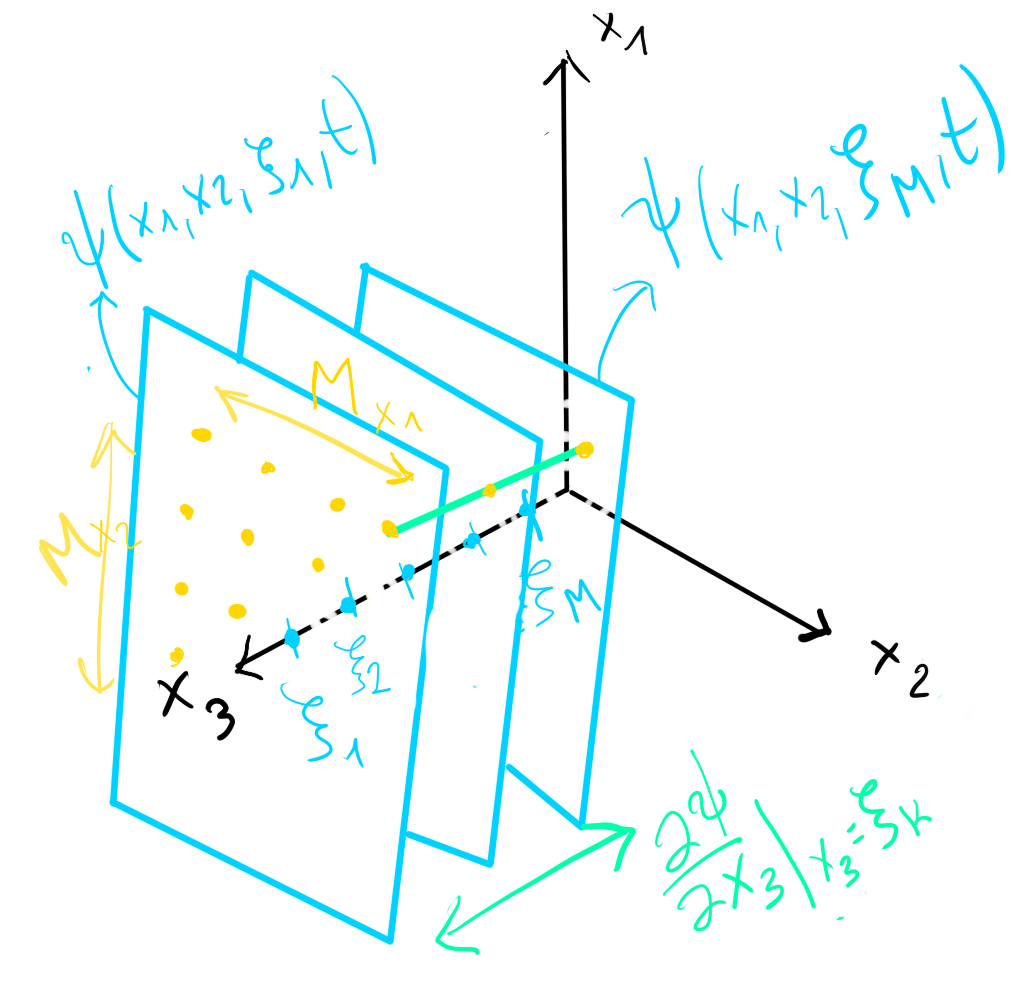
\includegraphics[width=0.5\linewidth]{hyperplaness.png}
  \caption{The $M$ hyperplanes in blue depict the $N-1$ dimensional supports of the CWF-s with a single Lagrangian degree ($x_3$). Each hyperplane is labeled by the initial position in the $x_3$ axis, the labels $\xi_j$. The yellow dots represent the $M_{x1}xM_{x2}$ discretized points of each hyperplane CWF. As it can be seen, the yellow points of the different hyperplanes are aligned, since the trajectories are fixed. This means that derivatives in the Lagrangian axis can be computed numerically at all times for any considered point in the hyperplanes.}
  \label{fig:hyperplane}
\end{figure}
\mybox{
We could do the same but instead of considering a single Lagrangian axis, we could consider two. In such a case, each CWF would have support in an affine $N-2$D manifold. Now about $O(M^2)$ CWF-s would be required, but each of them would take $O(M^{N-2})$ time to get evolved if we knew the correlation potentials. Now the derivatives to compute the correlation potentials would be required to be done in two directions, menaing we would require $O(2M^{N-2})$ threads computing each $O(M)$ operations. A total time of $O(M^{N-2})$ would be enough, at the expense of using more parallel threads.\\

If we wanted to minimize the computational time, what we could do is the following: consider all but one degree as Lagrangian, considering this way CWF-s like $\psi(x_1,x_2^\xi(t), ...,x_N^\xi(t))$, the support of which would be a line moving in $\R^N$. See Figure \ref{fig:line}. If we build a regular grid in the space $x_2,...x_N$, for each point in the grid, we could consider a line-CWF extending in $x_1$ (the labels $\xi$ of each CWf would be their positions on this initial grid).}

\mybox{ Taking $O(M^{N-1})$ line-CWFs of those (each in a different thread), we would have a value of the WF per point in the whole configuration space (considering each CWF is discretized in $O(M)$ points, we would have a regular grid for the full wave-function). Then, in order to compute the correlation potentials, we would require for each of the $O(M)$ points of the line-CWF (the Eulerian axis), the derivative in each of the $N-1$ directions of the Lagrangian axes. If there are $M^{N-1}$ CWF-s, the same $O(M^{N-1})$ threads could compute the $O(M[N-1])$ derivatives. In total a perfect parallelization in those $O(M^{N-1})$ threads would take then $O(M[N-1]+M)=O(MN)$ operations. If we assume there is an overhead per message pass between the threads, each thread needs to send and receive $O(NM)$ values, leaving a total complexity in time that is $O(MN)$ to compute a single time iteration of the full wavefunction. This is linear in time wiht increasing precision and number of spatial dimensions, but is exponential in the number of threads required for it.}

\begin{figure}[h!]
  \centering
    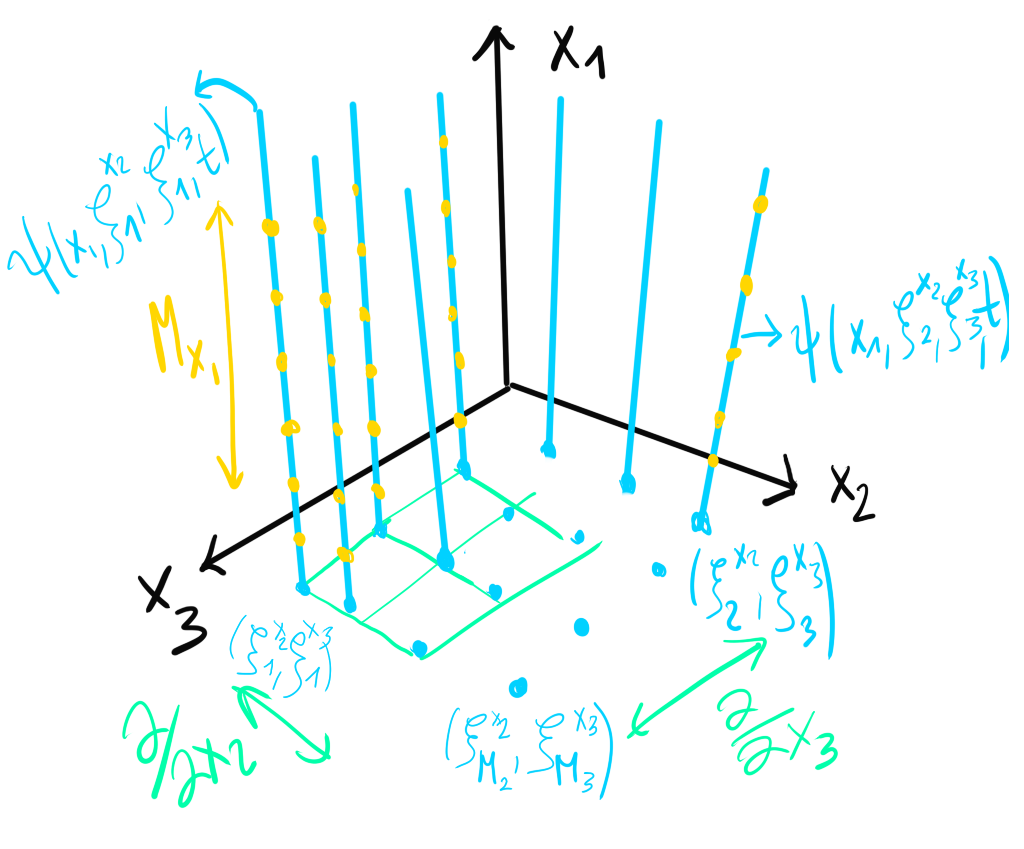
\includegraphics[width=0.5\linewidth]{rectas.png}
  \caption{In blue, the $M_{x2}xM_{x3}$ CWF-s, the supports of which are 1D manifolds. In yellow, the $M_{x1}$ discrete points we consider in each CWF. Note how the yellow points in $x_2$ and $x_3$ are aligned in a regular grid, meaning they can be used to compute numerically the derivatives in the Lagrangian directions.  }
  \label{fig:lines}
\end{figure}

\mybox{
For any intermediate arrangement of Eulerian and Lagrangian degrees of freedom, we could balance the computational complexity from temporal to spatial at will. The more Lagrangian coordinates we choose the more parallel threads will be required, but the less time it will take.\\

This approach is in principle legitimate for both the approach described in II.a.1 or II.a.2, the differences are the following ones though: the equation in II.a.1 has affine terms that impede the usage of reliable methods like the Crank Nicolson one. However, in II.a.2 we need to compute terms where we have $R$ dividing. This is prone to introduce big errors where the density is small.

}

Es la salvacion, y la unica "ventaja" de las CWF kizas. Ze sale una ecuacion lienal, solucionable de forma estable (aunke no preserve la norma, ze hay potencial complejo). Y es un mix de la full SE y la CE+HJE es un intermitx ke solo es concebible en CWF-s.
% TODO: 
- Generalize G,J zuk guzuzen beste Eulerianera 1h
- Ein Basis Set thing eta por fin harek ekuaziñoiek idatzi 3h
- Leidú Adaptive Gridsen kapituloa 
- Idatzi ALE+suggestion de hacerlas lienales haciendo trajs ke siguen la densidad? 3h
- Leidú dynamical equations for partial derivatives eta idatzi euren atala. 3h
- Leidu lo de Jacobianena eta idatzi suggestion para hacer derivadas respecto a las material coordinates. 3h
- Eing marrazkixek. 3h


\subsection*{(II.b.1) The Continuity + The Hamilton-Jacobi Equations}
If we evaluate the trajectory $\vec{y}(t;\vec{\xi})$ in the Continuity equation \eqref{CE}, we obtain:
\begin{equation}
\dv{}{t}\rho(\vec{x},\vec{y}^\xi(t),t)=-\sum_{j=1}^m\pdv{}{x_j}\qty(\rho(\vec{x}, \vec{y}^\xi(t), t) \frac{1}{m_j}\pdv{S(\vec{x}, \vec{y}^\xi(t), t)}{x_j}) - \rho(\vec{x}, \vec{y}^\xi(t),t) \sum_{j=m+1}^N \frac{1}{m_j}\pdv[2]{S(\vec{x}, \vec{y}, t)}{x_j}\Big\rvert_{\vec{x}^\xi(t)}
\end{equation}
Which is a continuity equation for $\rho(\vec{x},\vec{y}^\xi(t),t)$ with a source term $- \rho(\vec{x}, \vec{y}^\xi(t),t) \sum_{j=m+1}^N \frac{1}{m_j}\pdv[2]{S(\vec{x}, \vec{y}, t)}{x_j}\Big\rvert_{\vec{x}^\xi(t)}$ that drains or injects density as a function of the sign of the gradient of the velocity field in the Lagrangian axes (the contraction or dilation of the volume element, the determinant of the Jacobian of the density for the Lagrangian degrees). This is why the time evolution of the CWF-s is non-unitary. This was already clear in the fully Lagrangian scheme, because the density of the fluid was not a conserved quantity along the trajectories, meaning that the density that each fluid element perceives can vary in time. We actually found that the amount of density a fluid element perceived changed in time with the dilatation and contraction of the trajectory bundle, as given by the Jacobian of the mesh.

Evaluating the trajectory for the Lagrangian axes in the Hamilton-Jacobi equation \eqref{HJE} we get the ugly equation:
\begin{equation}
-\dv{}{t}S(\vec{x}, \vec{y}^\xi(t),t)=\sum_{j=1}^m\frac{1}{2m_j}\qty(\pdv{S(\vec{x},\vec{y}^\xi(t),t)}{x_j})^2-\sum_{j=m+1}^N\frac{1}{2m_j}\qty(\pdv{S(\vec{x},\vec{y}^\xi(t),t)}{x_j})^2+U(\vec{x},\vec{y}^\xi(t),t)+
\end{equation}
$$
-\sum_{j=1}^m \frac{\hbar^2}{2m_jR(\vec{x},\vec{y}^\xi(t),t)}\pdv[2]{R(\vec{x},\vec{y}^\xi(t),t)}{x_j}-\sum_{j=m+1}^N \frac{\hbar^2}{2m_jR(\vec{x},\vec{y}^\xi(t),t)}\pdv[2]{R(\vec{x},\vec{y},t)}{x_j}\Big\rvert_{\vec{x}^\xi(t)}
$$
Which is the Hamilton-Jacobi equation for the CWF, except that there are two terms extracting energy: the kinetic energy of Lagrangian frame and the quantum potential contribution due to the agglomeration in that axis.

%\subsection*{(II.b.2) The Bohmian-Newton's Second Law}
%Evaluating the trajectory $\vec{y}(t;\vec{\xi})$ in the Continuity equation \eqref{CE}, we obtain:

\subsection*{(III.b.1.2) Adaptive Grid Equations}
% como puedes controlar als trayectorias dada una monitor function, por ejemplo podrias hacer que conservasen la densidad no? OStyras esa sería muy buena! De fet para esas trayectorias saldria una continuity equation exacta! Y las CWF-s tendrian una time evolution unitaria!!!! Pa sacar cual es el velocity field que deberian seguir quizas podrias mirar cuando la Lagrangian frame equation para las trajs te da que es constante la densidad. Y creo que es cuando la derivada en el espacio de la dSdx aka la velocidad (?) es constante a lo largo de la trayectoria...Y claro como es una fk continua tb deberia funcionar ke exista esa trayectoria no? 



\subsection*{(II.c) Basis Set Expansion}
\addcontentsline{toc}{subsection}{(II.c) Basis Set Expansion}
\subsubsection*{(I.c.1) Hamiltonian and Sub-Hamiltonian Eigenstate Expansion}
\addcontentsline{toc}{subsubsection}{(I.c.1) Hamiltonian and Sub-Hamiltonian Eigenstate Expansion}
In this section we will develop an equation that will allow us the time evolution of a {\bf single} CWF, without the need of evolving several of them in parallel, at the cost of knowing the eigenstates of the Lagrangian axes!

If we recover the equation \eqref{XabEq} and the formalism we employed in its derivation, we had that the full WF could be decomposed as $\Psi(x,y,t)=\sum_{j=0}^\infty\Lambda^j(x,t)\Phi^j_x(y,t)=\sum_{j=0}^\infty \varphi_j(x,y,t)$. We defined $\Phi^j_x(y,t)$ as the transversal section eigenstates of the subsystem due to the degrees of freedom $y=(x_{m+1},...,x_N)$, which depend on the slice $x=(x_1,...,x_m)$ we are looking at. Now, if we know these eigenstates and we evaluate the wavefunction along a trajectory for the "transversal" degrees of freedom $y^\xi(t)$, we note that equation \eqref{XabEq2.5} becomes:

\begin{equation}
 i\hbar\pdv{}{t}\varphi^k(x,y^\xi(t),t)=\qty[ \varepsilon^k(x,t)+V(x,t)  -\sum_{s=1}^m\frac{\hbar^2}{2m_s}\pdv[2]{}{x_s} ]\varphi^k(x,y^\xi(t),t)+
\end{equation}
$$
+\sum_{j=0}^\infty\sum_{s=1}^m \frac{-\hbar}{2m_s}\qty( \frac{1}{\Phi^j_x(y^\xi(t),t)}\pdv[2]{\Phi^j_x(y^\xi(t),t)}{x_s}+2\pdv{}{x_s}log(\Phi^j_x(y^\xi(t),t))\qty[\pdv{}{x_s}-\pdv{}{x_s}log(\Phi^j_x(y^\xi(t),t))] )\varphi^j(x,y^\xi(t),t)
$$
Denoting $\varphi^k_\xi(x,t)=\varphi^k(x,y^\xi(t),t)$ and thus the CWF $\Psi^\xi(x,t)=\sum_j \varphi^j_\xi(x,t)$, by using the chain rule for the time derivative we get:
\begin{equation}\label{XabEq3}
 i\hbar\pdv{}{t}\varphi^k_\xi(x,t)=\qty[-\sum_{s=1}^m\frac{\hbar^2}{2m_s}\pdv[2]{}{x_s}+ \varepsilon^k(x,t)+V(x,t)   +i\hbar \dv{}{t}log(\Phi^k_x(y^\xi(t),t))]\varphi^k_\xi(x,t)+
\end{equation}
$$
+\sum_{j=0}^\infty\sum_{s=1}^m \frac{-\hbar}{2m_s}\qty( \frac{1}{\Phi^j_x(y^\xi(t),t)}\pdv[2]{\Phi^j_x(y^\xi(t),t)}{x_s}+2\pdv{}{x_s}log(\Phi^j_x(y^\xi(t),t))\qty[\pdv{}{x_s}-\pdv{}{x_s}log(\Phi^j_x(y^\xi(t),t))] )\varphi^j_\xi(x,t)
$$
This is a coupled system of {\bf linear} equations that allows the time evolution of a {\bf single CWF}, if we truncate the series $\Psi^\xi(x,t)=\sum_j \varphi^j_\xi(x,t)$ at a convenient point. Since it is linear, a Crank Nicolson like stable algorithm can be used to evolve it in a time in the order of the resolution of an $m$ dimensional Schrödinger Equation. Of course, the trick to overcome the many body problem is in that we know a priori the transversal section eigenstates $\Phi^j_x(y,t)$ for the particular potential energy. Obtaining these $N-m$ dimensional eigenstates numerically presents the same exponential nature as the full Schrödinger Equation.

However, it is really interesting to note that this is in practice the only approach that allow the exact (with no theoretical approximation) time evolution of a single CWF!






\subsection*{(III.d) Dynamic Equations for Partial Differentials}


\section*{III . No Pilot-Wave: Finite Tangent Universe Mechanics}




 


\begin{thebibliography}{1}
\addcontentsline{toc}{section}{References}

\bibitem{JordiXO}
	Oriols X, Mompart J, {\em Applied Bohmian Mechanics: From Nanoscale Systems to Cosmology} Pan Stanford, Singapore (2012)
	
%\bibitem{XO}
%	Oriols X. 2007 {\em Quantum-trajectory approach to time-dependent transport in mesoscopic systems with electron-electron interactions} Phys. Rev. Lett. 98 066803

\bibitem{Wyatt}
R. E. Wyatt, {\em Quantum Dynamics with Trajectories} (Springer, Berlin, 2006)

%\bibitem{Dev}
%	Devashish Pandey, Xavier Oriols, and Guillermo Albareda. {\em Effective 1D Time-Dependent Schrödinger Equations for 3D Geometrically Correlated Systems.} Materials 13.13 (2020): 3033.

\bibitem{nireTFGie}
	Oyanguren Xabier, {\em The Quantum Many Body Problem}, Bachelor's Thesis (2020) for the Nanoscience and Nanotechnology Degree (UAB).

\href{https://github.com/Oiangu9/The\_Quantum\_Many\_Body\_Problem\_-Bachellors\_Thesis-/blob/master/TheQuantumManyBodyProblem\_\_BachelorsThesis\_XabierOyangurenAsua.pdf}{https://github.com/Oiangu9/The\_Quantum\_Many\_Body\_Problem\_-Bachellors\_Thesis-/blob/master/TheQuantumManyBodyProblem\_\_BachelorsThesis\_XabierOyangurenAsua.pdf}

\bibitem{physicalOriols}
Norsen, T., Marian, D. \& Oriols, X. {\em Can the wave function in configuration space be replaced by single-particle wave functions in physical space?.} Synthese 192, 3125–3151 (2015). \href{https://doi.org/10.1007/s11229-014-0577-0}{https://doi.org/10.1007/s11229-014-0577-0}


\bibitem{movingGrids}
Knupp, Patrick \& Steinberg, Stanly. {\em The Fundamentals of Grid Generation.} (1993) \href{https://www.researchgate.net/publication/265361548_The_Fundamentals_of_Grid_Generation}{https://www.researchgate.net/publication/265361548\_The\_Fundamentals\_of\_Grid\_Generation} 

%\bibitem{Albareda}
%	Albareda G, Kelly A, Rubio A. {\em Nonadiabatic quantum dynamics without potential energy surfaces.} Phys Rev Materials. 2019; 3: 023803. 

%\bibitem{DATA}
%	All the animations employed for the analysis of Section 3.2 can be found in the following link:\\
%	\href{https://drive.google.com/drive/folders/1vnNDZrIYDlAhd-kVmmnVJgXmcdE2gxAV?usp=sharing}{https://drive.google.com/drive/folders/1vnNDZrIYDlAhd-kVmmnVJgXmcdE2gxAV?usp=sharing}
	
\end{thebibliography}


\end{document}
